\documentclass[thesis]{thesis-gwu}[2018/08/31]

\usepackage{xspace}
\usepackage{xcolor} %remove if not needed at the end
\usepackage{multirow} 
\usepackage{mathpazo} %uses palatino in text and math 
\usepackage{cite} %takes cares of citing 1-5 instead of 1,2,3,4,5
\usepackage{parskip}


\newcommand{\pygbe}{\texttt{PyGBe}\xspace}
\newcommand{\gmres}{\textsc{gmres}\xspace}
\newcommand{\bem}{\textsc{bem}\xspace}
\newcommand{\gpu}{\textsc{gpu}}
\newcommand{\cpu}{\textsc{cpu}}
\newcommand{\nvidia}{\textsc{nvidia}\xspace}
\newcommand{\msms}{\texttt{\textsc{msms}}\xspace}
\newcommand{\amber}{\texttt{\textsc{amber}}\xspace}
\newcommand{\ccby}{\textsc{cc-by}\xspace}
\newcommand{\bigO}{\mathcal{O}}
\renewcommand{\O}[1]{\mathcal{O}(#1)}
% !TEX root = ../thesis-sample.tex

% --------- FRONT MATTER PAGES ---------------------
% Title of the thesis
\title{COMPUTATIONAL NANOPLASMONICS FOR BIOSENSING APPLICATIONS: A BOUNDARY INTEGRAL IMPLEMENTATION IN THE QUASISTATIC LIMIT.}

% Author name
\author{Natalia Carolina Clementi}

% Previous degrees
\bsdepartment{Physics}
\bsschool{Universidad Nacional de C{\'o}rdoba.}
\bsgrad{2013}

\msdepartment{MS department}
\msschool{University}
\msgrad{year}
%\showmsdegree % you can show or hide the MS degree line 
\hidemsdegree

% PhD degree commands
% Committee
\showcommitteepage % hide this page if you're doing a MS thesis
%\hidecommitteepage 
\committee{ %
Lorena A. Barba, Professor of Mechanical and Aerospace Engineering,\\ 
Dissertation Director\\ % remember to add a space between committee members

Sanyia LeBlanc, Associate Professor of Mechanical and Aerospace Engineering,
Committee Member\\

Kausik Sarkar, Professor of Mechanical and Aerospace Engineering, \\
Committee Member\\

Yongsheng Leng, Professor of Mechanical and Aerospace Engineering, \\
Committee Member\\

Christopher Cooper Villagr{\'a}n, Assistant Professor of Mechanical Engineering,
Committee Member\\

}

% Chair must be entered separately for formatting reasons.
\chair{Lorena A. Barba}
\chairtitle{Professor of Mechanical and Aerospace Engineering}
% Department
\department{Mechanical and Aerospace Engineering}

\phdgrad{May 16, 2021}
\defensedate{February 19, 2021}
% Year of completion for copyright page and perhaps other places
\year=2021

% Copyright page
%\copyrightholder{Someone else}

% Dedication
\dedication{To all the women scientist to come. %
}

% Acknowledgments
\acknowledgments{
PENDING
}

% -----------------------------------------------------------------
% Typically only one of Preface/Foreward/Prologue would be in your thesis.
% To choose one simply delete the others and they will automatically dissappear

% Preface
\preface{
    This is the preface. 
    It's another front matter page that offers additional detail into your work.
    Typically, only one (preface OR prologue OR foreword) is used. 
    You can remove the other sections by deleting them inside \texttt{tex/frontmatter.tex} or using the appropriate show or hide commands.
}

\prologue{
    This is the prologe. 
    It's another front matter page that offers additional detail into your work.
    Typically, only one (preface OR prologue OR foreword) is used. 
    You can remove the other sections by deleting them inside \texttt{tex/frontmatter.tex} or using the appropriate show or hide commands.
}

\foreword[2]{
    This is the forword. 
    It's another front matter page that offers additional detail into your work.
    Typically, only one (preface OR prologue OR foreword) is used. 
    You can remove the other sections by deleting them inside \texttt{tex/frontmatter.tex} or using the appropriate show or hide commands.
}
% ----------------------------------------------------------------------

% commands to show or hide front matter pages

\showcopyright
\showabstract
\showcommitteepage
\showdedication
\showacknowledgments
\hidepreface
\hideprologue
\hideforeword

% ------------ TABLE OF CONTENTS ----------------------
% Commands to hide or show lists of figures, tables, etc.
\showlistoffigures
\showlistoftables
\hidenomenclature

\makeglossaries

% Some abstract text
\abstract{
This is the abstract. 
It contains some random text from 
}

%avoid indentation of paragraphs
\setlength\parindent{0pt}

%% DOCUMENT AREA
\begin{document}

% !TEX root = ../thesis-sample.tex
\chapter{Introduction} \label{chap:intro}

A biosensor is a measuring device used to detect the presence or concentration of a biomolecule. The general system includes 
a probe with a sensitive biological receptor, a transducer and a detector. For the past three decades, research in biosensing 
has rapidly grown with applications in multiple areas like medical diagnoses, disease monitoring, drug delivery studies, 
and detection of biological agents \cite{Turner2000, Mohanty2006, Mehrotra2016}. Optical biosensors are a particular type of biosensor 
known for their sensitivity and real-time detection. Among many optical sensing techniques we have fluorescence, Raman spectroscopy, lithography, 
and surface plasmon resonance. Biosensors based on surface plasmon resonance (SPR) changes in thin gold films are some of the most 
commonly used optical biosensors.  These sensors exploit a particular type of electromagnetic waves called surface plasmon polaritons for the
detection of a biomolecule \cite{Homola2008}. However, when using metallic nanoparticles instead of thin films, a powerful resonance peak 
shows in the visible range, a phenomenon known as Localized Surface Plasmon Resonance (LSPR). When electromagnetic waves excite the free electrons on 
the surface of a conductive nanoparticle, they resonate with the incoming electric field forming plasmons. Most of the incoming energy is either 
absorbed by the nanoparticle, or scattered in multiple directions, creating a large shadow behind the scatterer (a.k.a extinction cross section). In LSPR, 
the resonance wavelength highly depends on the refraction index of the environment, the geometry of the nanoparticle and its material. LSPR biosensors measure 
the shift in the plasmon resonance wavelength ($\Delta\lambda$) of the metallic nanoparticle as a biomolecule approaches it. Biosensing based on LSPR 
is more precise and provides high-sensitivity detection \cite{Sepulveda2009}. This technique has been used in multiple areas of biological detection, 
such as viruses and cancer \cite{Wang2010, Liu2014, Zhu2016}. 

The physics of localized surface plasmon resonance are modeled and solved by Maxwell's equations, and they are generally solved numerically 
by using finite difference time-domain (FDTD), boundary element, or finite element methods \cite{SolisTaboadaObelleiroLiz-MaarzanGarciadeabajo2014}.
These methods have been used to study the optical properties of dielectric or metallic nanoparticles \cite{Hohenester2018,HohenesterTrugler2012,
JungPedersenSondergaardPedersenLarsenNielsen2010, VideenSun2003,MayergoyzFredkinZhang2005, MayergoyzZhang2007}, interactions between nanoparticles
and electron beams \cite{GarciadeabajoAizpurua1997, GarciadeabajoHowie2002}, and surface plasmon resonance sensors. For the latter application, 
researchers use simple mathematical models for the interaction between the nanoparticle and the biomolecules, like representing the molecules as simple 
spheres \cite{DavisGomezVernon2010,AntosiewiczApellClaudioKall2011, SantiagoCordobaETal2011, ShenETal2013, UngerETal2009} or a prisms \cite{DanHu2014}, using 
constant real dielectrics for the analyte \cite{NghiemETal2012, SantiagoCordobaETal2011, ShenETal2013, UngerETal2009}, or representing the embedding medium 
and dissolved biomolecules with an effective permittivity \cite{JungCampbellChinowskyMarYee1998,WilletsVandyune2007,PhanETal2013}.

Experimental research drives progress in the field of biosensing, which can be costly and time consuming. Computational approaches could complement the design process and play a key role in the optimization of biosensors. Using computational approaches
can not only reduce the cost of the exploratory stages, but also give access to details that are not always available in experimental settings. For example, 
the distance between the sensor and the biomolecule, the amount of analytes in the vicinity of the sensor and their orientation, and other factors such as
the inclusion of the charges in the protein and the effects of the magnitude in the electric field when they are present. There are studies that show that 
the sensitivity of the sensor depends highly on the distance between the nanoparticle and the analyte \cite{HaesETal2004}. Other experimental studies complement
their results with models that ignore the presence of the biomolecules. Beuwer et al.~\cite{BeuwervanHoofZijlstra2018} and Henkel et al.~\cite{HenkelETal2018} 
use a boundary element method (BEM) in studies of the sensitivity of plasmonic sensors relying on (at least) two metallic nanoparticles 
(one on the sensor and one attached to the analyte). There is experimental evidence that shows that LSPR sensors are sensitive enough to detect conformational
changes in the biomolecules used as analytes \cite{HallETal2011}. Oversimplified models will not capture such details. 

When the wavelength of the incoming field is much larger than the size of the nanoparticle ($\lambda>>d$), the physics of the optical phenomenon of 
localized surface plasmon resonance can be reduced to electrostatics. This approximation enables us to use our boundary integral 
electrostatic solver, \pygbe, to compute the extinction cross section of metallic or dielectric nanoparticles, and to study how the LSPR response varies in the 
presence of a biomolecule. We show how sensitivity is affected by the distance between the sensor and the analyte in LSPR biosensors. We exhibit the impact 
of using different geometrical models for the biomolecules on the LSPR response. We analyze the effect of including charges in the protein model. We present 
the differences of using real versus complex dielectric models for both the analyte and embedding medium.

\pygbe is a Python implementation of continuum electrostatic theory that relies on the boundary element method, its original application included 
the computing of solvation energy of biomolecular systems \cite{CooperBardhanBarba2013}, and the studying of protein orientation near charged 
nanosurfaces \cite{CooperClementiBarba2015}. In 2017, we extended \pygbe to the field of nanoplasmonics, by treating localized surface plasmon resonance 
(LSPR) quasistatically \cite{ClementiETal2017}. The boundary element solver in \pygbe is accelerated algorithmically via a treecode, an $\mathcal{O}(N\log N)$ 
fast-summation method, and on hardware by taking advantage of graphic processing units (GPUs). This allows us to handle problems in the order of half a million 
boundary elements, or more, thus being able to use an accurate representation of the biomolecular surface. There are other research softwares that could be use 
for this application, like BEM++ \cite{SmigajETal2015} and a Matlab toolbox called MNPBEM \cite{HohenesterTrugler2012}, which have the capability to solve the 
full Maxwell's equations and the electrostatic approximation in the long-wavelength limit. However, we believe that the size of the
problems these softwares can solve, in terms of the number of boundary elements,  may not be enough to resolve the details of the biomolecules.

 
To the best of our knowledge, \pygbe is the only open-source software that uses a fast algorithm ($\mathcal{O}(N\log N)$),
for $N$ unknowns—and hardware acceleration on GPUs to compute the extinction cross-sections of arbitrary geometries to explore
nanophotonics applications in the quasistatic limit. Our software is openly developed via its repository on 
Github (\url{https://github.com/barbagroup/pygbe}), has been verified (see section \ref{sec:verification}) against an analytical solution based 
on the Mie theory for silver nanospheres, validated against experimental results of reflectance of localized surface phonon polariton 
(SPhP) nanostructures from Ellis et al. (see section \ref{ssec:validation}), and we share it under the BSD 3-clause license.

This work follows careful reproducibility practices, and the materials necessary to reproduce or replicate our results are publicly available in 
reproducibility packages. Specific information about the reproducibility packages can be found at the end of each chapter with results. 


% !TEX root = ../thesis-sample.tex

\chapter{Background and Methods} \label{chap:methods}
\graphicspath{{background_methods/figs/}}


Localized surface plasmon resonance (LSPR) is an optical phenomenon generated by electromagnetic waves 
that excite the free electrons on the surface of a conductive small nanoparticle. These electrons resonate  
with the incoming electric field, forming plasmons (see Figure \ref{fig:lspr}). When resonance occurs, 
most of the incoming energy is either absorbed by the nanoparticle, or scattered in multiple directions, both
creating a large shadow behind the scatterer (a.k.a. extinction cross section). If the nanoparticle is 
smaller than $20$ nm, absorption dominates and scattering contributions are negligible \cite{PetryayevaKrull2011, OlsonETal2015}.

\begin{figure}
   \centering
     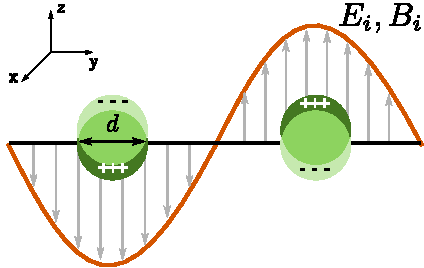
\includegraphics[width=0.55\textwidth]{lspr.pdf} 
     \caption{Illustration of the localized surface plasmon resonance (LSPR) effect of a metallic nanoparticle under an electromagnetic field.}
     \label{fig:lspr}
\end{figure}

The phenomenon of LSPR can be used for biosensing, as the resonance frequency is highly dependent on the dielectric environment 
around the scatterer. The resonance frequency shifts whenever an analyte binds to the nanoparticle, 
resulting in a very sensitive method of detecting the analyte's presence \cite{HaesVanduyne2002,HaesETal2004}
(see Figure \ref{fig:lspr_bio}). Even though LSPR is an optical effect, electrostatic theory
provides a good approximation when the wavelength of the incoming electric field is much larger than 
the size of the nanoparticle (long-wavelength limit). 

Throughout this work, we use the boundary integral electrostatic solver \pygbe \cite{ClementiETal2017} to compute 
the LSPR response of a silver nanoparticle, and how it varies in the presence of biomolecules. We treat Maxwell's equations
quasi-statically \cite{MayergoyzZhang2007} and explicitly represent the target biomolecules by a surface mesh.

\begin{figure}
   \centering
     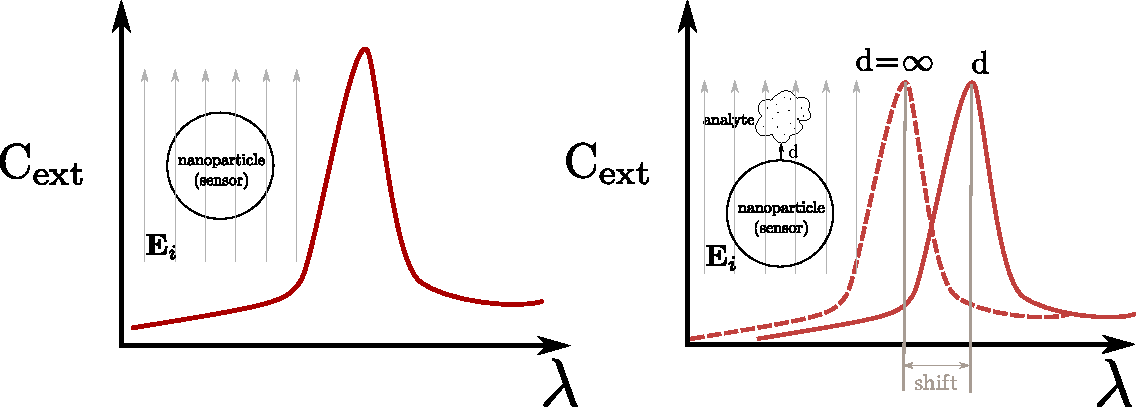
\includegraphics[width=0.95\textwidth]{lspr_biosensing.pdf} 
     \caption{Illustration of LSPR response shift in the presence of an analyte.}
     \label{fig:lspr_bio}
\end{figure}


The first implementation of \pygbe relied on continuum electrostatics to compute the solvation energy
of biomolecules. These biomolecules are modeled as dielectric cavities inside an infinite continuum 
solvent, leading to a Poisson equation inside the molecules and Laplace or Poisson-Boltzmann
(to account for salt ions) in the solvent. The partial differential equations that model this problem
can be expressed as boundary integral equations along the molecular interface, and solved using 
\pygbe's boundary element method implementation \cite{CooperBardhanBarba2013,CooperClementiBarba2015}.
This work extends \pygbe to nanoplasmonics in the quasistatic limit for LSPR biosensing application. In the long-wavelength limit,
Maxwell's equations can be approximated by a Laplace equation, allowing us to use the methods implemented in \pygbe with modifications
to accept complex-valued permittivities, and to include the effect of an external electric field. This chapter describes the mathematical
formulation for computing electromagnetic scattering in the long-wavelength setting, and develops the associated boundary 
integral equations and their discretized form.

%%%%%EDIT
\section{Scattering of small particles} \label{sec:scattering_small}

In this section, we show how electrostatic theory is a first order approximation of Maxwell's 
equations and that it applies in the long-wavelength limit. We present the derivation from 
Mayergoyz and Zhang \cite{MayergoyzZhang2007}, due to its importance to explain the boundary 
element methods approach for our LSPR biosensor model. The following derivation considers only one particle 
in the domain, but the analysis extends to multiple particles. Figure \ref{fig:part_wave} shows a 
sketch of the system that we analyze in this derivation. Region $\Omega_1$ is a nanoparticle 
immersed in a host medium $\Omega_2$, and subjected to an incoming electromagnetic wave with  electric field 
$\mathbf{E}_i$ and magnetic field $\mathbf{B}_i$.

\begin{figure}%[h] %  figure placement: here, top, bottom, or page
   \centering
   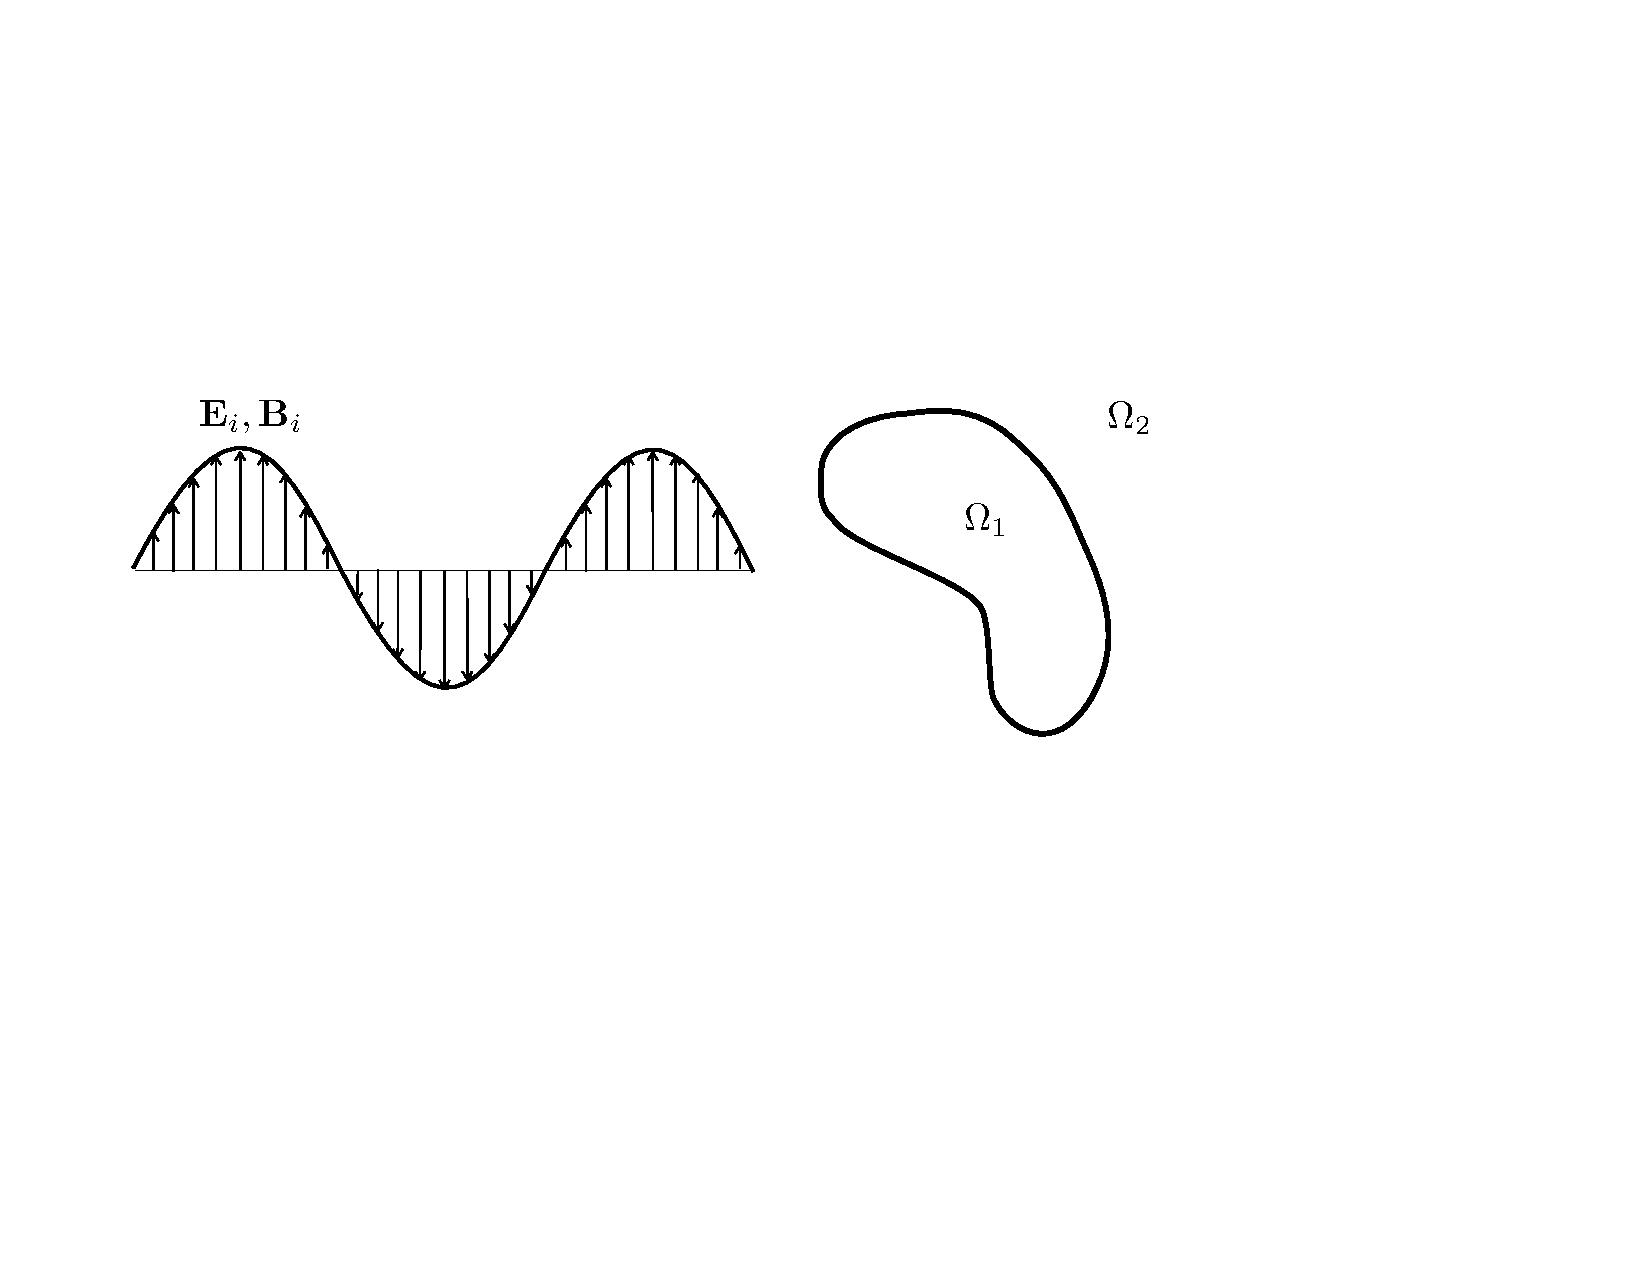
\includegraphics[width=0.65\textwidth]{particle_wave.pdf} 
   \caption{Nanoparticle interacting with an electromagnetic wave.}
   \label{fig:part_wave}
\end{figure}


Equation \eqref{eq:maxwell_timeharmonic} is a system of partial differential equations that
models a scattered, time-harmonic electromagnetic field. Where the electric field $\mathbf{E}$ and 
the magnetic field $\mathbf{B} = \mu \mathbf{H}$ vary only in space. 

\begin{align} \label{eq:maxwell_timeharmonic}
   \epsilon_1 \nabla \cdot \mathbf{E}_{1s} =& \rho_{f1} \qquad \nabla \times \mathbf{E}_{1s} = -\mu_1i\omega\mathbf{H}_{1s} \nonumber \\
   \mu_1\nabla \cdot \mathbf{H}_{1s} =& 0 \qquad \nabla \times \mathbf{H}_{1s} = \mathbf{J}_{f1} + \epsilon_1i\omega\mathbf{E}_{1s} + (\epsilon_1-\epsilon_2)i\omega\mathbf{E}_{i}\qquad \text{ on $\Omega_1$,} \nonumber \\
   \epsilon_2 \nabla \cdot \mathbf{E}_{2s} =& \rho_{f2} \qquad \nabla \times \mathbf{E}_{2s} = -\mu_2i\omega \mathbf{H}_{2s} \nonumber \\
   \mu_2\nabla \cdot \mathbf{H}_{2s} =& 0 \qquad \nabla \times \mathbf{H}_{2s} = \mathbf{J}_{f2} + \epsilon_2i\omega\mathbf{E}_{2s} \qquad \text{ on $\Omega_2$, and} \nonumber \\
   (\epsilon_1\mathbf{E}_{1s}-\epsilon_2\mathbf{E}_{2s})&\cdot\mathbf{n} = (\epsilon_2-\epsilon_1)\mathbf{E}_i\cdot\mathbf{n} \nonumber \\
   \mathbf{H}_{1s}&\cdot \mathbf{n} = \mathbf{H}_{2s}\cdot\mathbf{n} \qquad\text{ on the interface $\Gamma$}.
\end{align} 

In a setting with no charges or currents like in Figure \ref{fig:part_wave}, Equation \eqref{eq:maxwell_timeharmonic} becomes
 %
 \begin{align} \label{eq:maxwell_nocharge}
 \nabla \cdot \mathbf{E}_{1s} &= 0 \qquad \nabla \times \mathbf{E}_{1s} = -\mu_1i\omega\mathbf{H}_{1s} \nonumber \\
 \nabla \cdot \mathbf{H}_{1s} &= 0 \qquad \nabla \times \mathbf{H}_{1s} = \epsilon_1i\omega\mathbf{E}_{1s} + (\epsilon_1-\epsilon_2)i\omega\mathbf{E}_{i} \qquad \text{on $\Omega_1$} \nonumber \\
 \nabla \cdot \mathbf{E}_{2s} &= 0 \qquad \nabla \times \mathbf{E}_{2s} = -\mu_2i\omega\mathbf{H}_{2s} \nonumber \\
 \nabla \cdot \mathbf{H}_{2s} &= 0 \qquad \nabla \times \mathbf{H}_{2s} = \epsilon_2i\omega\mathbf{E}_{2s} \qquad \text{on $\Omega_2$} \nonumber \\
 (\epsilon_1\mathbf{E}_{1s} - \epsilon_2\mathbf{E}_{2s})\cdot\mathbf{n} &= (\epsilon_2-\epsilon_1)\mathbf{E}_i\cdot \mathbf{n} \nonumber \\(\mathbf{H}_{1s} - \mathbf{H}_{2s})\cdot \mathbf{n}&=0 \qquad \text{on the interface $\Gamma$,}
 \end{align}
 
 We want to study the effect of the size of the particle in the scattered field, to do so we need 
 to use the following scaled quantities:
 %
 \begin{align}\label{eq:scaled_quant}
 \mathbf{e}_i = \sqrt{\epsilon_2}\mathbf{E}_i, \qquad \mathbf{e}_s = \sqrt{\epsilon_2}\mathbf{E}_s, \nonumber \\
 \mathbf{h}_s = \sqrt{\mu_2}\mathbf{H}_s \qquad \mathbf{x}^\prime = \frac{\mathbf{x}}{d},
 \end{align}
 
 where $d$ is the particle size, and $\mathbf{x}^\prime$ a scaled domain. Turning
 Equation \eqref{eq:scaled_quant} into Equation \eqref{eq:maxwell_nocharge}, we get
 %
 \begin{align} \label{eq:maxwell_scaled}
 \nabla \cdot \mathbf{e}_{1s} &= 0 \qquad \nabla \times \mathbf{e}_{1s} = -i\beta\mathbf{h}_{1s}\frac{\mu_1}{\mu_2} \nonumber \\
 \nabla \cdot \mathbf{h}_{1s} &= 0 \qquad \nabla \times \mathbf{h}_{1s} = \frac{\epsilon_1-\epsilon_2}{\epsilon_2}i\beta\mathbf{e}_{i}+\frac{\epsilon_1}{\epsilon_2}i\beta\mathbf{e}_{1s}  \qquad \text{on $\Omega_1$} \nonumber \\
 \nabla \cdot \mathbf{e}_{2s} &= 0 \qquad \nabla \times \mathbf{e}_{2s} = -i\beta\mathbf{h}_{2s} \nonumber \\
 \nabla \cdot \mathbf{h}_{2s} &= 0 \qquad \nabla \times \mathbf{h}_{2s} = i\beta\mathbf{e}_{2s} \qquad \text{on $\Omega_2$} \nonumber \\
 (\epsilon_1\mathbf{e}_{1s} - \epsilon_2\mathbf{e}_{2s})\cdot\mathbf{n} &= (\epsilon_2-\epsilon_1)\mathbf{e}_i\cdot \mathbf{n} \nonumber \\(\mathbf{h}_{1s} - \mathbf{h}_{2s})\cdot \mathbf{n}&=0 \qquad \text{on the interface $\Gamma$,}
 \end{align}
 
 with $\beta=\omega d \sqrt{\epsilon_2\mu_2}$. We can expand $\mathbf{e}$ and $\mathbf{h}$ in 
 terms of $\beta$ as
 %
 \begin{align} \label{eq:expand}
 \mathbf{e} &= \mathbf{e}_s^{(0)} + \beta \mathbf{e}_s^{(1)} + \beta^2 \mathbf{e}_s^{(2)} + \ldots \nonumber\\
 \mathbf{h} &= \mathbf{h}_s^{(0)} + \beta \mathbf{h}_s^{(1)} + \beta^2 \mathbf{h}_s^{(2)} + \ldots,
 \end{align}
 
 If we consider only the zeroth order terms in Equation \eqref{eq:maxwell_scaled} we get
 %
 \begin{align} \label{eq:maxwell_scatter_zeroth}
 \nabla \cdot \mathbf{e}^{(0)}_{1s} &= 0 \qquad \nabla \times \mathbf{e}^{(0)}_{1s} = 0 \nonumber \\
 \nabla \cdot \mathbf{h}^{(0)}_{1s} &= 0 \qquad \nabla \times \mathbf{h}^{(0)}_{1s} = 0 \nonumber \\
 \nabla \cdot \mathbf{e}^{(0)}_{2s} &= 0 \qquad \nabla \times \mathbf{e}^{(0)}_{2s} = 0 \nonumber \\
 \nabla \cdot \mathbf{h}^{(0)}_{2s} &= 0 \qquad \nabla \times \mathbf{h}^{(0)}_{2s} = 0 \nonumber \\
 (\epsilon_1\mathbf{e}^{(0)}_{1s} - \epsilon_2\mathbf{e}^{(0)}_{2s})\cdot\mathbf{n} &= (\epsilon_2-\epsilon_1)\mathbf{e}_i\cdot \mathbf{n} \nonumber \\(\mathbf{h}^{(0)}_{1s} - \mathbf{h}^{(0)}_{2s})\cdot \mathbf{n}&=0.
 \end{align}

Equation \eqref{eq:maxwell_scatter_zeroth} has the form of an electrostatic field, where the electric
and magnetic fields are decoupled. Then $\mathbf{h}^{(0)}=0$ and $\mathbf{e}^{(0)}$ can be described by a
scalar potential since $\nabla \times \mathbf{e}^{(0)}=0$.
 
Equation \eqref{eq:maxwell_scatter_zeroth} is a good approximation as long as $\beta$ is small. On the host medium, the wave 
speed is $c=1/\sqrt{\epsilon_2\mu_2}$, then $\beta=\omega d \sqrt{\epsilon_2\mu_2} = d\omega/c  = d/\lambda$. In this work
we look at the long-wavelength limit ($\lambda > d$), that translates in Equation \eqref{eq:maxwell_scatter_zeroth} becoming
a valid approximation, making electrostatic theory suitable to model localized surface plasmon resonance (quasi-static approximation).

In Equation \eqref{eq:maxwell_scatter_zeroth}, the zeroth order term of the magnetic field is zero
everywhere, therefore we will concentrate only on the electric field. Ignoring all the terms related 
to the magnetic field, we can rewrite Equation \eqref{eq:maxwell_scatter_zeroth} in terms of 
$\mathbf{E}$ and $\mathbf{x}$ instead of the scaled quantities $\mathbf{e}$ and
$\mathbf{x}^\prime$, as:

\begin{align} \label{eq:electrostatic_scatter_E}
\nabla \cdot \mathbf{E}_{1s} &= 0 \qquad \nabla \times \mathbf{E}_{1s} = 0, \nonumber \\
\nabla \cdot \mathbf{E}_{2s} &= 0 \qquad \nabla \times \mathbf{E}_{2s} = 0, \nonumber \quad
\text{with interface conditions, } \nonumber \\
(\epsilon_1\mathbf{E}_{1s} &- \epsilon_2\mathbf{E}_{2s})\cdot\mathbf{n} = (\epsilon_2-\epsilon_1)\mathbf{E}_i\cdot \mathbf{n}.
\end{align}

In Equation \eqref{eq:electrostatic_scatter_E}, $\mathbf{E}_{1s}$ and $\mathbf{E}_{2s}$ 
are the electric fields of the scattered wave in the nanoparticle and host regions, respectively 
(see Figure \ref{fig:part_wave}), $\mathbf{E}_{i}$ is the electric field of the incoming wave, and $\epsilon_1$ 
and $\epsilon_2$ are the permittivities. This approximation decouples the electric and magnetic fields, neglects the magnetic field, 
and describes the electric field as a curl-free vector field. Hence, we can reformulate Equation \eqref{eq:electrostatic_scatter_E} with a scalar potential
($-\nabla \phi_{js} = \mathbf{E}_{js}$), as follows:
%
\begin{align} \label{eq:electrostatic_scatter}
\nabla^2 \phi_{1s} &= 0 \qquad \nabla^2 \phi_{2s} = 0 \qquad\text{on $\Omega_1$, $\Omega_2$} \nonumber \\
\epsilon_1\frac{\partial\phi_{1s}}{\partial \mathbf{n}} - \epsilon_2\frac{\partial\phi_{2s}}{\partial\mathbf{n}} &= (\epsilon_2-\epsilon_1)\frac{\partial\phi_i}{\partial\mathbf{n}} \quad \phi_{1s} = \phi_{2s} \quad \text{on $\Gamma$}.
\end{align}
%
Equation \eqref{eq:electrostatic_scatter} is an electrostatic equation with an imposed electric
field $\mathbf{E}_i=-\nabla\phi_i$, where $\Gamma$ is the boundary between the regions $\Omega_1$ and $\Omega_2$.

\subsection{Far-field scattering} \label{sec:ff_scattering}

In LSPR, the scattered electromagnetic wave is measured by a detector located far away 
from the scatterer (nanoparticle), and the plasmon resonance is identified when the energy 
detected is minimum. In the far-field limit, the scattered field
in the outside region ($\Omega_2$) is given by: 

\begin{equation} \label{eq:scat_efield_long_range}
    \mathbf{E}_{2s} = \frac{1}{4\pi\epsilon_2}k^2\frac{e^{ikr}}{r} (\mathbf{\hat{r}} \times \mathbf{p})\times\mathbf{\hat{r}}.
\end{equation} 

where $k=2\pi/\lambda$ is the wave number and $\lambda$ the wavelength, $\mathbf{\hat{r}}$ 
is a unit vector in the direction of the observation point, and $\mathbf{p}$ is
the dipole moment. 
The scattered electric field in the long wavelength limit, can also be expressed in terms of the 
scattering amplitude $\mathbf{F}$ \cite{Jackson} as:

\begin{equation} \label{eq:scat_efield_fwa}
    \mathbf{E}_{2s}(\mathbf{r})_{r\to\infty} = \frac{e^{ikr}}{r} \mathbf{F}(\mathbf{k},\mathbf{k}_0),
\end{equation}

where $\mathbf{k}$ is the scattered wave vector in the direction of propagation, and $\mathbf{k}_0$ the 
wave vector of the incident field. 

\subsection{Extinction cross-section and optical theorem} \label{sec:cext_ot}

The extinction cross-section ($C_\text{ext}$) is a measure of the energy that 
does not reach the detector, either because it is scattered in other directions,
or due to absorption. This quantity is defined as the ratio between the lost energy and 
the intensity of the incoming wave, and has units of area. The extinction cross-section peaks when
plasmons of the nanoparticle resonate with the incoming electric field.

The optical theorem connects the extinction cross section with the forward-scattering amplitude. The traditional 
expression for this relationship applies for non-absorbing media 
\cite{MayergoyzZhang2007, Jackson}; Mishchenko \cite{Mishchenko2007} corrected it for absorbing media, 
giving an expression that can be rewritten using Jackson's notation \cite{Jackson} as follows:

\begin{equation} \label{eq:cext_fwa}
    C_\text{ext} = \frac{4\pi}{k^\prime} \operatorname{Im} \left[ \frac{\mathbf{\hat{e}}_i}{|\mathbf{E}_i|}\mathbf{F}(\mathbf{k}=\mathbf{k}_0, \mathbf{k}_0) \right].
\end{equation}

where $k^\prime$ is the real part of the complex wave number, 

\begin{equation}
    k = k^\prime + ik^{\prime\prime} = \frac{2\pi}{\lambda} n,
\end{equation}

and $n$ is the refraction index of the host medium.

Combining Equations \eqref{eq:scat_efield_long_range} and \eqref{eq:scat_efield_fwa},
we can compute the scattering amplitude to  obtain the extinction cross-section 
with Equation \eqref{eq:cext_fwa}.

\section{The Boundary Element Method} \label{sec:lspr_bem}

When a partial differential equation has a fundamental solution and can be expressed as a boundary integral equation (BIE), we can 
solve this BIE numerically via the boundary element method (\bem). The idea of using a boundary integral equation to represent partial 
differential equations started early in the 1800s in the work of Green \cite{Green1828}, and followed by Betti, Somigliana and Fredholm \cite{Betti1872,Somigliana1885,Fredholm1903} 
in the late 1800s and early 1900s. Fredholm was the first one to compute boundary data in a potential theory application, which marks him as a 
pioneer of the boundary element method. In the 1960s the first numerical solutions to Fredholm's equation for two dimensional potential theory appeared in 
the works of Jawson \cite{Jawson1963} and Symm \cite{Symm1963}, and Rizzo \cite{Rizzo1967} and Cruse \cite{Cruse1969} presented the solutions for 
two- and three-dimensional elastostatics. Since then, the boundary element method has evolved and been used as a numerical technique in 
multiple areas\cite{Atkinson1997,McLean2000,Steinbach2008, BrebbiaDominguez1992, Katsikadelis2002}.


\subsection{Integral formulation of the Laplace equation} \label{ssec:int_form}

A well known PDE that we can solve with \bem is the Laplace equation. For a scalar quantity $\phi$ in a domain $\Omega$ with boundary $\Gamma$, and 
boundary conditions $\phi_0$ or $\partial \phi_0/\partial \mathbf{n}$, the Laplace equation takes the form:
%
\begin{align} \label{eq:lap_pde}
\nabla^2\phi &= 0 \quad \text{ on $\Omega$} \nonumber \\
\phi = \phi_0 \text{ or } \frac{\partial \phi}{\partial \mathbf{n}} &= \frac{\partial \phi_0}{\partial \mathbf{n}} \quad \text{ on $\Gamma$} 
\end{align}

The weak formulation of Laplace equation \eqref{eq:lap_pde} with test function $w$ is:

\begin{equation} \label{eq:lap_weak}
\int_\Omega \nabla^2 \phi(\mathbf{r}_\Omega') w(\mathbf{r}_\Omega') \text{d} \Omega^\prime= 0.
\end{equation}

where the evaluation point is $\mathbf{r}_\Omega$ a location in the domain $\Omega$.

If we use the Laplace's free-space Green's function as the test function $w$ we
get:

\begin{equation} \label{eq:lap_weak2}
\int_\Omega \nabla^2 \phi(\mathbf{r}'_\Omega) G_L(\mathbf{r}_\Omega,\mathbf{r}'_\Omega) \text{d} \Omega^\prime= 0.
\end{equation}

Manipulating the integrand using the product rule and later the divergence 
theorem, we get:

\begin{equation} \label{eq:lap_bie_dom}
\phi(\mathbf{r}_\Omega) = \oint_\Gamma G_L(\mathbf{r}_\Omega,\mathbf{r}'_\Gamma)  \frac{\partial} {\partial \mathbf{n}} \phi(\mathbf{r}'_\Gamma)  \text{d} \Gamma^\prime - \oint_\Gamma \phi(\mathbf{r}'_\Gamma)  \frac{\partial}{\partial \mathbf{n}} G_L(\mathbf{r}_\Omega,\mathbf{r}'_\Gamma) \text{d} \Gamma^\prime
\end{equation}

where \eqref{eq:lap_bie_dom}, $\mathbf{r}$ can be anywhere in the domain $\Omega$, 
and $\mathbf{r}'$ runs only on the boundary $\Gamma$. This equation has a 
singularity when $\mathbf{r}=\mathbf{r}'$. To handle this problem, we perform the
integral on a surface $\Gamma'$ that is like $\Gamma$ but with a hemisphere of 
radius $\varepsilon$ center at $\mathbf{r}$. We split the integrals into the part
that has no singularity and the part that has the hemisphere. After solving these
equations when $\varepsilon \to 0$, equation \eqref{eq:lap_bie_dom} results in:

\begin{equation} \label{eq:lap_bie}
\frac{\phi(\mathbf{r}_\Gamma)}{2} +  \oint_\Gamma \phi(\mathbf{r}'_\Gamma)  \frac{\partial}{\partial \mathbf{n}} G_L(\mathbf{r}_\Gamma,\mathbf{r}'_\Gamma) \text{d} \Gamma^\prime = \oint_\Gamma G_L(\mathbf{r}_\Gamma,\mathbf{r}'_\Gamma)  \frac{\partial} {\partial \mathbf{n}} \phi(\mathbf{r}'_\Gamma)  \text{d} \Gamma^\prime,
\end{equation}

where the integrals are Cauchy principal value integrals.

Using the single and double layer operators:

\begin{equation}\label{eq:single_layer}
   V^{\Gamma}_L (\psi(\mathbf{r}_\Gamma)) = \oint_\Gamma \psi(\mathbf{r}'_\Gamma) G_L(\mathbf{r}_\Gamma, \mathbf{r}'_\Gamma) \text{d} \Gamma',
   \end{equation}
   %
   \begin{equation}\label{eq:double_layer}
   K^{\Gamma}_L (\psi(\mathbf{r}_\Gamma)) = \oint_\Gamma \psi(\mathbf{r}'_\Gamma) \frac{\partial}{\partial \mathbf{n}}G_L(\mathbf{r}_\Gamma, \mathbf{r}'_\Gamma) \text{d} \Gamma'.
   \end{equation}
   %
where $G_L$ is the free-space Green's function of the Laplace equation:
   %
   \begin{equation}
   G_L(\mathbf{r},\mathbf{r}') = \frac{1}{4\pi|\mathbf{r}-\mathbf{r}'|}
   \end{equation}
   

We can rewrite equation \eqref{eq:lap_bie} using the operator notation, as:

\begin{equation} \label{eq:lap_operator}
\left[ \frac{\mathbb{I}}{2} + K_L^{\mathbf{r}_\Gamma} \right] \left( \phi_\Gamma \right) = V_L^{\mathbf{r}_\Gamma} \left( \frac{\partial}{\partial \mathbf{n}} \phi_\Gamma \right),
\end{equation}

where $\mathbb{I}$ is the identity operator.

\subsubsection{Electrostatic potential of a nanoparticle under an electric field} \label{sec:pot_elec_field}

Following the same steps from section \ref{ssec:int_form}  we can write the system of partial differential equations 
in Equation \eqref{eq:electrostatic_scatter} as a system of boundary integral equations \cite{BrebbiaDominguez1992}. Evaluating on the
surface $\Gamma$, this becomes
%
\begin{align} \label{eq:integral_eq_lspr_nobc}
\frac{\phi_{1s,\Gamma}}{2}+ K_{L}^{\Gamma}(\phi_{1s,\Gamma}) - V_{L}^{\Gamma} \left(\frac{\partial}{\partial \mathbf{n}}\phi_{1s,\Gamma} \right) = 0&  \nonumber \\
\frac{\phi_{2s,\Gamma}}{2} - K_{L}^{\Gamma}(\phi_{2s,\Gamma}) + V_{L}^{\Gamma} \left( \frac{\partial}{\partial \mathbf{n}} \phi_{2s,\Gamma} \right) = 0&,
\end{align}
%
where $V$ and $K$ are the single- and double-layer operators.
%
Applying the interface conditions of Equation \eqref{eq:electrostatic_scatter},
leads to:

\begin{align} \label{eq:integral_eq_lspr}
\frac{\phi_{1s,\Gamma}}{2}+ K_{L}^{\Gamma}(\phi_{1s,\Gamma}) - V_{L}^{\Gamma} \left(\frac{\partial}{\partial \mathbf{n}}\phi_{1s,\Gamma} \right) &= 0  \nonumber \\
\frac{\phi_{1s,\Gamma}}{2} - K_{L}^{\Gamma}(\phi_{1s,\Gamma}) + \frac{\epsilon_1}{\epsilon_2}V_{L}^{\Gamma} \left( \frac{\partial}{\partial \mathbf{n}} \phi_{1s,\Gamma}  \right) &=
 \frac{\epsilon_2-\epsilon_1}{\epsilon_2}V_{L}^{\Gamma}\left( \frac{\partial}{\partial \mathbf{n}} \phi_{i,\Gamma} \right)\quad \text{on $\Gamma$.}
\end{align}


\subsubsection{Analyte-sensor electrostatic potential under an electric field}

The sketch in Figure \ref{fig:analyte-sensor} shows a metallic nanoparticle ($\Omega_1$) interacting with an analyte ($\Omega_3$), under an external electric field.
Mathematically, this situation can be modeled as:

\begin{align}\label{eq:electrostatic_scatter_prot_sen}
\nabla^2 \phi_{1s} &= 0, \qquad \nabla^2 \phi_{2s} = 0 \qquad\text{on $\Omega_1$, $\Omega_2$} \nonumber\\
\nabla^2 \phi_{3s} &= -\frac{1}{\epsilon_3} \sum_{k=0}^{N_q} \delta(|\mathbf{r}-\mathbf{r}_k|) q_k \qquad\text{on $\Omega_3$} \nonumber \\
\epsilon_1\frac{\partial\phi_{1s}}{\partial \mathbf{n}} - \epsilon_2\frac{\partial\phi_{2s}}{\partial\mathbf{n}} &= (\epsilon_2-\epsilon_1)\frac{\partial\phi_i}{\partial\mathbf{n}} \quad \phi_{1s} = \phi_{2s} \quad \text{on $\Gamma_1$}. \nonumber\\
\epsilon_3\frac{\partial\phi_{3s}}{\partial \mathbf{n}} - \epsilon_2\frac{\partial\phi_{2s}}{\partial\mathbf{n}} &= (\epsilon_2-\epsilon_3)\frac{\partial\phi_i}{\partial\mathbf{n}} \quad \phi_{3s} = \phi_{2s} \quad \text{on $\Gamma_2$}.
\end{align}
%
where $q_k$ are the point charges of the atoms inside the protein, located at $\mathbf{r}_k$.

\begin{figure}%[b] %  figure placement: here, top, bottom, or page
   \centering
   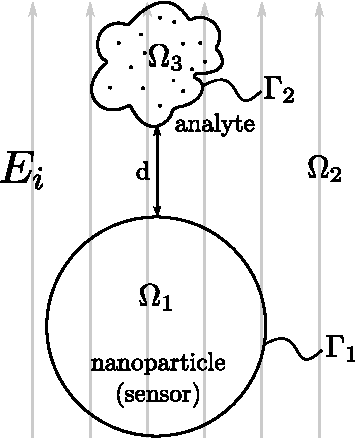
\includegraphics[width=0.35\textwidth]{protein_sensor_regions.pdf} 
   \caption{Analyte-sensor system under electric field.}
   \label{fig:analyte-sensor}
\end{figure}

Similar to Equation \eqref{eq:integral_eq_lspr}, we can write the system of partial differential equations in 
\eqref{eq:electrostatic_scatter_prot_sen} as:

\begin{align} \label{eq:integral_eq_lspr_nobc_system}
\frac{\phi_{1s,\Gamma_1}}{2}+ K_{L,\Gamma_1}^{\Gamma_1}(\phi_{1s,\Gamma_1}) &- V_{L,\Gamma_1}^{\Gamma_1} \left(\frac{\partial}{\partial \mathbf{n}}\phi_{1s,\Gamma_1} \right) = 0  \nonumber \\
\frac{\phi_{2s,\Gamma_1}}{2} - K_{L,\Gamma_1}^{\Gamma_1}(\phi_{2s,\Gamma_1}) + V_{L,\Gamma_1}^{\Gamma_1} \left(\frac{\partial}{\partial \mathbf{n}}\phi_{2s,\Gamma_1} \right) 
& - K_{L,\Gamma_2}^{\Gamma_1}(\phi_{2s,\Gamma_2}) + V_{L,\Gamma_2}^{\Gamma_1} \left(\frac{\partial}{\partial \mathbf{n}}\phi_{2s,\Gamma_2} \right) = 0  \nonumber \\
\frac{\phi_{2s,\Gamma_2}}{2} - K_{L,\Gamma_1}^{\Gamma_2}(\phi_{2s,\Gamma_1}) + V_{L,\Gamma_1}^{\Gamma_2} \left(\frac{\partial}{\partial \mathbf{n}}\phi_{2s,\Gamma_1} \right)  
&- K_{L,\Gamma_2}^{\Gamma_2}(\phi_{2s,\Gamma_2}) + V_{L,\Gamma_2}^{\Gamma_2} \left(\frac{\partial}{\partial \mathbf{n}}\phi_{2s,\Gamma_2} \right) = 0  \nonumber \\
\frac{\phi_{3s,\Gamma_2}}{2} + K_{L,\Gamma_2}^{\Gamma_2}(\phi_{3s,\Gamma_2}) &- V_{L,\Gamma_2}^{\Gamma_2} \left( \frac{\partial}{\partial \mathbf{n}} \phi_{3s,\Gamma_2} \right) = \frac{1}{4\pi\epsilon_3} \sum_{k=0}^{N_q} \frac{q_k}{|\mathbf{r}_{\Gamma_2} - \mathbf{r}_k|} ,
\end{align}
%
where $V$ and $K$ are the single- and double-layer operators in equations 
\eqref{eq:single_layer} and \eqref{eq:double_layer}. In this case, we distinguish between the
surface where the integrals run (subindex), and the surface that contains the evaluation point (superindex).

Applying the interface conditions of equation \eqref{eq:electrostatic_scatter_prot_sen},
leads to: 

\begin{align} \label{eq:integral_eq_lspr_system}
\frac{\phi_{1s,\Gamma_1}}{2}&+ K_{L,\Gamma_1}^{\Gamma_1}(\phi_{1s,\Gamma_1}) - V_{L,\Gamma_1}^{\Gamma_1} \left(\frac{\partial}{\partial \mathbf{n}}\phi_{1s,\Gamma_1} \right) = 0  \nonumber \\
 \frac{\phi_{1s,\Gamma_1}}{2}& - K_{L,\Gamma_1}^{\Gamma_1}(\phi_{1s,\Gamma_1}) + V_{L,\Gamma_1}^{\Gamma_1} \left(\frac{\epsilon_1}{\epsilon_2}\frac{\partial}{\partial \mathbf{n}}\phi_{1s,\Gamma_1} \right) - V_{L,\Gamma_1}^{\Gamma_1} \left(\frac{\epsilon_2-\epsilon_1}{\epsilon_2}\frac{\partial}{\partial \mathbf{n}}\phi_{i,\Gamma_1} \right) \nonumber\\ 
 & - K_{L,\Gamma_2}^{\Gamma_1}(\phi_{3s,\Gamma_2}) + V_{L,\Gamma_2}^{\Gamma_1} \left(\frac{\epsilon_3}{\epsilon_2}\frac{\partial}{\partial \mathbf{n}}\phi_{3s,\Gamma_2} \right)  - V_{L,\Gamma_2}^{\Gamma_1} \left(\frac{\epsilon_2 -\epsilon_3}{\epsilon_2}\frac{\partial}{\partial \mathbf{n}}\phi_{i,\Gamma_2} \right) = 0   \nonumber \\
 \frac{\phi_{3s,\Gamma_1}}{2}& - K_{L,\Gamma_1}^{\Gamma_2}(\phi_{1s,\Gamma_1}) + V_{L,\Gamma_1}^{\Gamma_2} \left(\frac{\epsilon_1}{\epsilon_2}\frac{\partial}{\partial \mathbf{n}}\phi_{1s,\Gamma_1} \right) - V_{L,\Gamma_1}^{\Gamma_2} \left(\frac{\epsilon_2-\epsilon_1}{\epsilon_2}\frac{\partial}{\partial \mathbf{n}}\phi_{i,\Gamma_1} \right) \nonumber \\
& - K_{L,\Gamma_2}^{\Gamma_2}(\phi_{3s,\Gamma_2}) + V_{L,\Gamma_2}^{\Gamma_2} \left(\frac{\epsilon_3}{\epsilon_2}\frac{\partial}{\partial \mathbf{n}}\phi_{3s,\Gamma_2} \right)  - V_{L,\Gamma_2}^{\Gamma_2} \left(\frac{\epsilon_2 -\epsilon_3}{\epsilon_2}\frac{\partial}{\partial \mathbf{n}}\phi_{i,\Gamma_2} \right) = 0  \nonumber \\
\frac{\phi_{3s,\Gamma_2}}{2}& + K_{L,\Gamma_2}^{\Gamma_2}(\phi_{3s,\Gamma_2}) - V_{L,\Gamma_2}^{\Gamma_2} \left( \frac{\partial}{\partial \mathbf{n}} \phi_{3s,\Gamma_2} \right) = \frac{1}{4\pi\epsilon_3} \sum_{k=0}^{N_q} \frac{q_k}{|\mathbf{r}_{\Gamma_2} - \mathbf{r}_k|} 
\end{align}



\subsection{Discretization and linear system}

We discretize the surface into flat triangles and assume that  $\phi$ and 
$\partial \phi/\partial \mathbf{n}$ are constant within each element. We can
write the layer operators in their discretized form as follows:
%
\begin{align} \label{eq:layers_disc}
V_{L,\text{disc}}^{\mathbf{r}_\Gamma} \left( \frac{\partial}{\partial \mathbf{n}} \phi(\mathbf{r}_{\Gamma}) \right) &= \sum_{j=1}^{N_p} \frac{\partial}{\partial \mathbf{n}} \phi(\mathbf{r}_{\Gamma_j}) \int_{\Gamma_j} G_L(\mathbf{r}_\Gamma,\mathbf{r}_{\Gamma_j})  \mathrm{d} \Gamma_j  \nonumber \\
K_{L,\text{disc}}^{\mathbf{r}_\Gamma}(\phi(\mathbf{r}_{\Gamma})) &=  \sum_{j=1}^{N_p}\phi(\mathbf{r}_{\Gamma_j})\int_{\Gamma_j} \frac{\partial}{\partial \mathbf{n}} \left[ G_L(\mathbf{r}_\Gamma,\mathbf{r}_{\Gamma_j}) \right]\mathrm{d} \Gamma_j
\end{align}
%
where $N_p$ is the number of discretization elements on $\Gamma$, 
and $\phi(\mathbf{r}_{\Gamma_j})$ and $\frac{\partial}{\partial \mathbf{n}} 
\phi(\mathbf{r}_{\Gamma_j})$ are the values of $\phi$ and 
$\frac{\partial \phi}{\partial \mathbf{n}}$ on panel $\Gamma_j$.
Using centroid collocation, we can write equation \eqref{eq:integral_eq_lspr} in matrix form as:
%
 \begin{equation} \label{eq:matrix_lspr}
 \left[
    \begin{matrix} 
       \frac{1}{2} + K_{L}^{\Gamma} & -V_{L}^{\Gamma}  \vspace{0.2cm} \\
       \frac{1}{2} - K_{L}^{\Gamma} &  \frac{\epsilon_1}{\epsilon_2} V_{L}^{\Gamma}  \vspace{0.2cm} 
    \end{matrix}
    \right] \left[ 
    \begin{matrix} 
       \phi_{1s,\Gamma} \vspace{0.2cm} \\
       \frac{\partial}{\partial \mathbf{n}} \phi_{1s,\Gamma} \vspace{0.2cm}
    \end{matrix} 
     \right] =   
    \left[
    \begin{matrix} 
       0 \\
       V_{L}^{\Gamma} \left(\frac{\epsilon_2-\epsilon_1}{\epsilon_2}\right) \frac{\partial\phi_i}{\partial\mathbf{n}} \vspace{0.2cm} 
    \end{matrix}
    \right]
 \end{equation}
%
Equation \eqref{eq:integral_eq_lspr_system} can be represented as:
%
\begin{align} \label{eq:matrix_multi}
 \left[
    \begin{matrix} 
       \frac{1}{2}+K_{L, \Gamma_1}^{\Gamma_1} & -V_{L, \Gamma_1}^{\Gamma_1} & 0 &  0   \vspace{0.2cm} \\
       \frac{1}{2}-K_{L, \Gamma_1}^{\Gamma_1} & \frac{\epsilon_1}{\epsilon_2} V_{L, \Gamma_1}^{\Gamma_1} & -K_{L, \Gamma_2}^{\Gamma_1} & \frac{\epsilon_3}{\epsilon_2} V_{L, \Gamma_2}^{\Gamma_1} \vspace{0.2cm}  \\
        -K_{L, \Gamma_1}^{\Gamma_2}&\frac{\epsilon_1}{\epsilon_2} V_{L, \Gamma_1}^{\Gamma_2} & \frac{1}{2}-K_{L, \Gamma_2}^{\Gamma_2}  &  \frac{\epsilon_3}{\epsilon_2} V_{L, \Gamma_2}^{\Gamma_2} \vspace{0.2cm} \\
       0 & 0 & \frac{1}{2}+K_{L, \Gamma_2}^{\Gamma_2}&  - V_{L, \Gamma_2}^{\Gamma_2}   \vspace{0.2cm} \\
    \end{matrix}
    \right] 
\cdot
 \left[
    \begin{matrix}
    \phi_{1,\Gamma_1} \vspace{0.2cm} \\
    \frac{\partial}{\partial \mathbf{n}} \phi_{1,\Gamma_1} \vspace{0.2cm} \\
    \phi_{3,\Gamma_2} \vspace{0.2cm} \\
    \frac{\partial}{\partial \mathbf{n}} \phi_{3,\Gamma_2} \vspace{0.2cm} \\
    \end{matrix}
\right]&
 \nonumber \\
 = \left[
    \begin{matrix}
    0 \vspace{0.2cm} \\
    V_{L,\Gamma_1}^{\Gamma_1} \left(\frac{\epsilon_2-\epsilon_1}{\epsilon_2}\frac{\partial}{\partial \mathbf{n}}\phi_{i,\Gamma_1} \right)
    + V_{L,\Gamma_2}^{\Gamma_1} \left(\frac{\epsilon_2 -\epsilon_3}{\epsilon_2}\frac{\partial}{\partial \mathbf{n}}\phi_{i,\Gamma_2} \right)
    \vspace{0.2cm}\\
    V_{L,\Gamma_1}^{\Gamma_2} \left(\frac{\epsilon_2-\epsilon_1}{\epsilon_2}\frac{\partial}{\partial \mathbf{n}}\phi_{i,\Gamma_1} \right)
    + V_{L,\Gamma_2}^{\Gamma_2} \left(\frac{\epsilon_2 -\epsilon_3}{\epsilon_2}\frac{\partial}{\partial \mathbf{n}}\phi_{i,\Gamma_2} \right)
    \vspace{0.2cm}\\
    \frac{1}{4\pi\epsilon_3}\sum_{k=0}^{N_q} \frac{q_k}{|\mathbf{r}_{\Gamma_2} - \mathbf{r}_k|} \vspace{0.2cm}  \\
    \end{matrix}
\right]&
\end{align}
%
where the elements of the matrix are
% %
\begin{align} \label{eq:layers_element}
V_{L,ij}^{\Gamma} &= \int_{\Gamma_j} G_L(\mathbf{r}_{\Gamma_i},\mathbf{r}_{\Gamma_j})  \mathrm{d} \Gamma_j, \nonumber \\
K_{L,ij}^{\Gamma} &= \int_{\Gamma_j} \frac{\partial}{\partial \mathbf{n}} \left[ G_L(\mathbf{r}_{\Gamma_i},\mathbf{r}_{\Gamma_j}) \right]\mathrm{d} \Gamma_j,
\end{align}
%
with $\mathbf{r}_{\Gamma_i}$ being at the center of panel $\Gamma_i$.


\subsubsection{Integral evaluation}

We evaluate the integrals in Equation \eqref{eq:layers_element} with Gauss quadrature
rules. The $1/r$ singularity of the Green's function poses a
problem to obtain good accuracy when the integral is 
singular or near-singular. We define three different regions for integration:

\begin{description}

\item[Singular integrals:] If the collocation point is in the integration element,
the singularity is difficult to resolve with standard
Gauss integration schemes. In this case, we use a semi-analytical technique 
\cite{HessSmith1967,ZhuHuangSongWhite2001} that places $N_k$ quadrature nodes on the 
edges of the triangle.

\item[Near singular integrals:] If the collocation point is close to the integration element,
the integrand has a high gradient, and high-order quadrature rules are required. 
We use the representative length of the integrated triangle ($L = \sqrt{2\cdot\text{Area}}$)
to define a threshold of the \emph{nearby} region, for example, when the integration panel 
is $2L$ or less, away from the collocation point. For near-singular integrals, we use  
$K_{fine}=19, 25  \text{ or }  37$ number of Gauss points per triangle. 

\item[Far away integrals:] When the distance between the collocation point and the integration
element is beyond the threshold, they are considered to be far away. 
At this point, the integrand is smooth enough that we obtain good 
accuracy with low-order integration, for example, with 
$K=1, 3  \text{ or } 4$ Gauss quadrature points per boundary element. 
\end{description}

\subsubsection{Boundary integral expression of the dipole moment}

As shown in Equation \eqref{eq:scat_efield_long_range}, the scattered electric 
field in the far-away limit depends on the dipole moment. The dipole moment is 
defined as 
%
\begin{equation} \label{eq:dipole_def}
\mathbf{p} = \int_\Omega \mathbf{r} \rho \text{d}\Omega,
\end{equation}
%
and rewriting this equation using Gauss' law, we obtain
%
\begin{equation} \label{eq:dipole_def_gauss}
\mathbf{p} = -\epsilon_2\int_\Omega \mathbf{r} \nabla^2 \phi_{2s} \text{d}\Omega.
\end{equation}
%
For a component $i$, this becomes:
%
\begin{equation} \label{eq:dipole_def_gauss_i}
{p_i} = -\epsilon_2\int_\Omega {x_i} \nabla^2 \phi_{2s} \text{d}\Omega.
\end{equation}
%
Using the identity
%
\begin{equation} \label{eq:identity_grad}
  \nabla \cdot \left(f \mathbf{v}\right) = \left( \nabla f \right)\cdot \mathbf{v} + f\left(\nabla \cdot \mathbf{v}\right)
\end{equation}
%
with $f=x_i$ and $\mathbf{v} = \nabla\phi_{2s}$, we can rewrite Equation \eqref{eq:dipole_def_gauss_i}
as 
%
\begin{equation}
- \frac{p_i}{\epsilon_2} = \int_\Omega \nabla \cdot \left( x_i \nabla \phi_{2s} \right) \; \text{d}\Omega - \int_\Omega \nabla x_i \cdot \nabla\phi_{2s} \; \text{d}\Omega, \nonumber 
\end{equation}
 and applying the divergence theorem
\begin{equation} \label{eq:dip_gauss_interm_1}
- \frac{p_i}{\epsilon_2}= \oint_\Gamma  x_i  \nabla \phi_{2s} \cdot \mathbf{n} \; \text{d}\Gamma - \int_\Omega \nabla x_i \cdot \nabla\phi_{2s} \; \text{d}\Omega.
\end{equation}
%
Using the identity \eqref{eq:identity_grad} again in Equation \eqref{eq:dip_gauss_interm_1}, this time 
taking $f=\phi_{2s}$ and $\mathbf{v} = \nabla x_i$, we get:
%
\begin{align} \label{eq:dip_gauss_interm_2}
 - \frac{p_i}{\epsilon_2} =& \oint_\Gamma  x_i  \frac{\partial \phi_{2s}}{\partial \mathbf{n}} \text{d}\Gamma - \nonumber \\
 & \left[ \int_\Omega \nabla \cdot \left( \phi_{2s} \nabla x_i \right)\;\text{d}\Omega - \int_\Omega  \phi_{2s} \nabla^2 x_i \;\text{d}\Omega\right] \nonumber\\
%&\text{and applying the divergence theorem} \nonumber \\
=& \oint_\Gamma  x_i  \frac{\partial \phi_{2s}}{\partial \mathbf{n}} \; \text{d}\Gamma - \oint_\Gamma \phi_{2s} \nabla x_i \cdot \mathbf{n} \; \text{d}\Gamma \nonumber \\
=& \oint_\Gamma  x_i  \frac{\partial \phi_{2s}}{\partial \mathbf{n}} \; \text{d}\Gamma - \oint_\Gamma \phi_{2s} n_i \;\text{d}\Gamma
\end{align}
%
Throughout this derivation, the normals are pointing into $\Omega_1$. However, in our implementation 
all normals are pointing outwards, and we need to include an extra negative sign, yielding:
%
\begin{equation} \label{eq:dipole_def_gauss_i_final}
{p_i} = \epsilon_2 \left[ \oint_\Gamma  x_i  \frac{\partial \phi_{2s}}{\partial \mathbf{n}} \text{d}\Gamma - \oint_\Gamma \phi_{2s} n_i \; \text{d}\Gamma \right].
\end{equation}

Using \bem, we obtain the electrostatic potential and its normal derivative on the surface of the nanoparticle. We use
them in Equation \eqref{eq:dipole_def_gauss_i_final} to get the dipole 
moment, and in Equation \eqref{eq:scat_efield_long_range} to obtain the scattered
electric field. Finally, using Equation \eqref{eq:scat_efield_fwa} and Equation 
\eqref{eq:cext_fwa} we get the extinction cross section.


\subsection{Acceleration strategies} \label{sec:acc_strategies}

One disadvantage of the Boundary Element Method (\bem) is that it generates dense matrices
after discretization. Solving the resulting linear system using
Gaussian elimination would require $\O{N^3}$ computations and $\O{N^2}$ storage. However, for a
Krylov-subspace iterative solver, like the Generalized Minimal Residual Method (GMRES),
computations drop to $\O{N^2}$ because they are dominated by dense matrix-vector 
products. This makes \bem inefficient for more than a few thousand boundary elements,
which are the mesh sizes required for real applications. But, there are acceleration methods
that make computations possible and scale as $\O{N \log N}$, or even $\O{N}$ that makes \bem a better candidate.

In our formulation with Gaussian quadrature and collocation, the matrix-vector product
becomes an $N$-body problem, with Gauss nodes acting as centers of mass (\emph{sources}), 
and the collocation points acting as evaluation points for the potential (\emph{targets}).
To overcome the unfavorable scaling, we accelerate the matrix-vector product using a 
treecode algorithm \cite{BarnesHut1986,DuanKrasny2001}, which is a fast-summation algorithm capable of reducing $\O{N^2}$
computational patterns like

\begin{equation} \label{eq:summation}
V(\mathbf{x}_i) = \sum_{j=1}^{N} q_j \psi(\mathbf{x}_i, \mathbf{y}_j) 
\end{equation}
%
to a computational complexity of $\O{N \log N}$. In Equation \eqref{eq:summation} 
$q_j$ is the weight, $\psi$ the kernel, $\mathbf{y}_j$ the locations of sources and 
$\mathbf{x}_i$ the locations of targets.

The treecode groups sources geometrically in boxes of an octree, built ensuring
that no box in the lowest level has more than $N_\text{crit}$ sources. If a group of
sources is far away from a target, their influence is aggregated at an expansion center,
and the target interacts with the box, rather than with each source independently. If the group of targets is close, 
the treecode queries the child boxes. If the box has no children and still is not far enough, the interaction is 
performed directly via \eqref{eq:summation}. The threshold to decide if a box is far enough is called the multipole-
acceptance criterion (MAC), defined as:
%
\begin{equation}
\theta > \frac{r_b}{r},
\end{equation}
%
where $r_b$ is the box size and $r$ the distance between the box center and the target.
Common values of $\theta$ are $1/2$ and $2/3$.
To approximate the contribution of the sources, we use Taylor expansions
of order $P$.
The treecode allows us to control the accuracy of the approximation by modifying $\theta$ and $P$.
Further details of the treecode implementation in \pygbe can be found in \cite{CooperBarba-share154331,CooperBardhanBarba2013}.

\subsection{Richardson extrapolation} \label{sec:rich_extrapolation}

In numerical computing, Richardson extrapolation is a technique used to get an estimation
of the exact solution from multiple computations using consecutive mesh resolutions from coarse
to fine. To be applied, all the computations used must converge to the exact value
at a constant rate. In other words, they are in the asymptotic range. When these conditions are met,
we can compute an estimate of the exact solution as:

\begin{equation} \label{eq:rich_extr}
   f_{\text{exact}} \approx f_1 + \frac{f_1 - f_2}{r^{p} - 1},
\end{equation} 

where $f_1$ and $f_2$ are the solutions at the fine and coarse grid, respectively, 
$r$ is the mesh refinement ratio, and $p$ is the order of convergence.

To use Equation \eqref{eq:rich_extr} we need to make sure that $f_1$ and $f_2$ are in the 
asymptotic regime. We compute the observed order of convergence $p$ from three grid resolutions
refined at constant ratio $r$:

\begin{equation} \label{eq:observed_order}
   p = \frac{\log \left( \frac{f_3 - f_2}{f_2-f_1} \right)}{\log (r)}.
\end{equation}
   
and if the result of Eq. \eqref{eq:observed_order} matches the \textit{expected} order of convergence
of the method, this indicates that the computations for $f_1$, $f_2$ and $f_3$ are in the asymptotic range.
Once we know that our $f_i$'s are in the asymptotic range, we can use Eq. \eqref{eq:rich_extr} and replace
the computed $p$ to get the estimated exact solution. We can also compute the estimated exact solution
directly from the values of $f_1$, $f_2$ and $f_3$ by doing some algebra on \eqref{eq:rich_extr}.

We know that $\log_r(x) = \log(x)/\log(r)$ and $r^{\log_r(x)} = x$. If we set $x = (f_3 - f_2)/(f_2 -f_1)$ 
then we can write Eq. \eqref{eq:observed_order}:

\begin{align} \label{eq:rich_extr2}
   f_{\text{exact}} &\approx f_1 + \frac{(f_1 - f_2)(f_2 -f_1)}{f_3-2f_2+f_1} \\
   f_{\text{exact}} &\approx \frac{f_1f_3 -{f_2}^2}{f_3-2f_2+f_1}
\end{align} 

Independently of how we compute the extrapolated value, we need three
calculations in the asymptotic convergence regime that result from computations
of three grid resolutions refined with constant ratio.


\subsection{Code modifications and added features} \label{sec:code_imp}

As mentioned at the beginning of this section, the present work extends the \pygbe code
to allow its application to nano-plasmonics. 
The code required the following modifications and added features:

\begin{itemize}
    \item Re-writing the GMRES solver to accept complex numbers. 
    \item Splitting treecode calculations into real and imaginary parts.
    \item Re-formatting configuration files to include electric field intensity and  wavelength.
    \item Adding the new function \texttt{read\_electric\_field}, to read the electric field intensity and its wavelength from configuration files.
    \item Adding the new function \texttt{dipole\_moment} to compute numerically the dipole moment by Equation \eqref{eq:dipole_def_gauss_i_final}.
    \item Adding the new function \texttt{extinction\_cross\_section} to compute the extinction cross section.
    \item Organizing LSPR computations on a different main script (called \texttt{lspr.py}).
\end{itemize}

For information about how to use the code, run examples and tests, see the
\pygbe documentation at \url{http://barbagroup.github.io/pygbe/docs/}

\subsection{Protein mesh preparation}

In Figure \ref{fig:analyte-sensor}, $\Omega_3$ is a region that represents the analyte molecule, which contains a point charge distribution 
of the partial charges, and is interfaced with the solvent by $\Gamma_2$, the solvent excluded surface (\texttt{SES}).
The \texttt{SES} is generated by rolling a spherical probe that is the size of a water molecule ($1.4$\AA~ radius) around the analyte, and tracking 
the points where the probe and molecule make contact.
The open-source software Nanoshaper \cite{Nanoshaper} uses the molecular structure to produce a triangulation of the \texttt{SES}, which can be 
read by our software. In particular, Nanoshaper takes as inputs the atomic coordinates, obtained from the Protein Data Bank (\url{https://www.rcsb.org/}),
and radii, which were extracted from a \texttt{pqr} file generated with \texttt{pdb2pqr} \cite{Dolinsky04}.
We obtained the charge and van der Waals parameters of the analyte from \texttt{pdb2pqr} using the built-in \texttt{amber} force field.

In support of the reproducibility of our results, we deposited the final meshes in the Zenodo data repositories. The details of each repository 
are present at the end of each chapter. 


%This should be under a bigger section name pending but something like
%Computational LSPR verification and application using pygbe
% !TEX root = ../thesis_main.tex
%%%%%%%%%%%%%%%%%%%%%%%
\chapter{\pygbelspr: A computational biosensing application} \label{chap:pygbe-lspr}
\graphicspath{{pygbe_lspr_bio/figs/}}

\pygbelspr \cite{ClementiETal2017} is the python library for applications in 
nanoplasmonics. This application was added to the original \pygbe \cite{CooperETal2016} which
is used to study biomolecular electrostatics, and it extends \pygbe to nanoplasmonics, by treating 
localized surface plasmon resonance (LSPR) quasi-statically \cite{MayergoyzZhang2007}. In this chapter 
we show the verification of \pygbelspr as well as an application on LSPR biosensing. 

\section{Verification of \pygbe - Isolated silver nanoparticle } \label{sec:verification}

When we are in the long wavelength limit, we know that the electrostatic approximation 
applies and we can model the scattering of a small metallic sphere as a nanoparticle 
under a constant electric field (see Figure \ref{fig:sph_field}). This problem 
has an analytical solution and we use it to perform a grid-convergence analysis for 
the verification of the \pygbe solver.

In this section we show a verification study. We compare the numerical solution
obtained we \pygbe against an analytical solution available for spherical 
nanoparticles. 

The first analytical solution of the extinction cross section of spherical 
nanoparticles in vacuum, known as Mie-Theory, was presented by Gustav Mie in 1908
\cite{Mie1908}. This exact solution uses full electromagnetic theory, but in the 
long wavelength limit, electrostatics will lead us to the same solution 
\cite{BohrenHuffman1983} which is:

\begin{equation} \label{eq:Cext_analytical}
    C_\text{ext} = 4\pi a^3 k \operatorname{Im}\left(\frac{\epsilon_p/\epsilon_m -1}{\epsilon_p/\epsilon_m -2}\right)
\end{equation}

where $a$ is the radius of the nanosphere, $k$ the wave number, 
$\epsilon_p$ the dielectric constant od the nanoparticle, and $\epsilon_m$ the
dielectric constant of the host medium, in this case,  vacuum permittivity
($\epsilon_m = \epsilon_0$).  This formula, does not count for losses in the medium.
However, in 2007 Mishchenko presented a solution that counts for losses in
the host environment:

\begin{equation} \label{eq:Cext_analytical_lossy}
    C_\text{ext} = \frac{4\pi a^3}{k^\prime} \operatorname{Im}\left(k^2 \frac{\epsilon_p/\epsilon_m -1}{\epsilon_p/\epsilon_m -2}\right)
\end{equation}

where $k=k^\prime + k^{\prime\prime}i$. When the host medium is 
non-absorbing, $k$ is real ($k^{\prime\prime} = 0$ and $k=k^\prime$) and we 
recover \eqref{eq:Cext_analytical}. 

In the quasistatic limit (long wavelength approximation) the scattering 
of small particles can be explained using electrostatics, and model as
a nanosphere under a constant electric field (Figure \ref{fig:sph_field}) 
with analytical solution given by Eq. \eqref{eq:Cext_analytical_lossy}.

\begin{figure}%[h] %  figure placement: here, top, bottom, or page
    \centering
    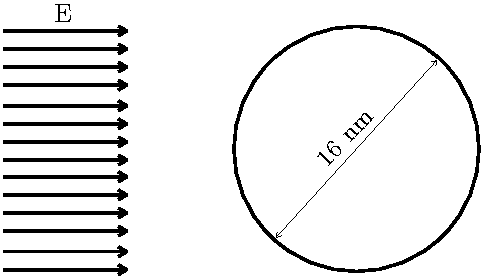
\includegraphics[width=0.55\textwidth]{sphere_field_8nm.pdf} 
    \caption{Spherical nanoparticle in a constant electric field.}
    \label{fig:sph_field}
\end{figure}

\subsection{Grid convergence analysis}\label{sub_sec:grid_conv_iso}

We perform a grid convergence analysis of \pygbe for a silver nanosphere 
of radius $r=8\,nm$ immersed in water, under a z-polarized electric field
of wavelength 380 nm and intensity of $-0.0037 e/(\text{\AA}^2 \, \epsilon_0)$.
For these conditions, the dielectric constant of water is
$1.7972 \, + \, 8.5048^{-09}i$ \cite{HaleQuerry1972} and for silver is
$-3.3877 \, + \, 0.1922i$ \cite{JohnsonChristy1972}. 
Table  \ref{table:quadparams1} shows the Gauss quadrature points used for each 
type of boundary element. We used a threshold parameter to define the near-singular
region of 0.5. This threshold defines the region of near singularity where 
semi-analytical technique is used. If $\sqrt{(2*Area)}/r > \text{threshold}$,
integration is done semi-analytically.
Table \ref{table:treeparams1} lists the parameters for the treecode and solver 
used in this convergence study.

\begin{table}%[h]
    \centering
    \caption{\label{table:quadparams1} Grid-convergence study: Gauss quadrature points; 
    $K$ and $K_{fine}$ are per element; $N_k $ is per element edge (semi-analytical integration). } 
    \begin{tabular}{l l}
    \hline%\toprule
     distant elements: & $K=4$ \\
     near-singular integrals:   & $ K_{fine}=37$ \\
     singular elements:  & $N_k =9$ \\
    \hline%\bottomrule
    \end{tabular}
\end{table}


\begin{table}%[h]
    \centering
    \caption{\label{table:treeparams1} Grid-convergence study: treecode and solver parameters.} 
    \begin{tabular}{l l}
    \hline%\toprule
    treecode order of expansion: & $P=15$\\
    MAC                          & $\theta=0.5$\\
    GMRES tolerance                    & $10^{-5}$\\
    \hline%\bottomrule
    \end{tabular}
\end{table}

Figure \ref{fig:conv_iso_sph} shows the results for the convergence study, with meshes of sizes 512, 2048, 
8192 and 32768 elements. The errors (Table \ref{table:err_iso_sph}) are computed against 
the analytical solution $C_{ext} = 1854.48$ nm$^2$ computed using Equation \eqref{eq:Cext_analytical_lossy}.
The dash line in Figure \ref{fig:conv_iso_sph} corresponds to a $1/N$ slope, and the observed order of 
convergence is $0.98$ which indicates that the meshes are correctly resolving the numerical solution with \pygbe.
The $1/N$ rate of convergence is consistent with convergence results in
previous work using \pygbe \cite{CooperBardhanBarba2013}. 

\begin{figure}%[h] %  figure placement: here, top, bottom, or page
    \centering
    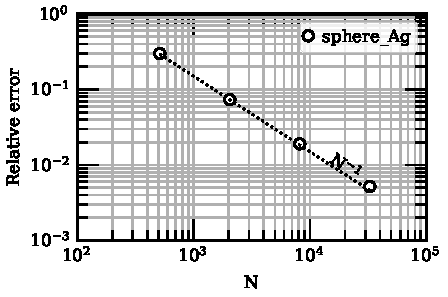
\includegraphics[width=0.85\textwidth]{convergence_sph_Ag_R8_w380.pdf} 
    \caption{Grid-convergence study for the extinction cross-section of a spherical silver
             nanoparticle, computed with \pygbe. Figure, plotting script and auxiliary files 
             available under \textsc{cc-by} \cite{ClementiETal2018c}.}
    \label{fig:conv_iso_sph}
 \end{figure}
 
 
 \begin{table}%[h]
     \centering
     \caption{\label{table:err_iso_sph} Percentage error in the grid-convergence cases with an 
     isolated silver nanosphere.} 
     \begin{tabular}{c c}
     \hline%\toprule
     N & \% error \\
     \hline%\midrule
      $512$ & $29.86$ \\
      $2048$ & $7.33$ \\
      $8192$ & $1.9$ \\
      $32768$ & $0.52$ \\
     \hline%\bottomrule
     \end{tabular}
 \end{table}


\subsection{LSPR response of silver nanosphere}\label{sub_sec:lspr_silver_np}

To complement the verification test for the Localized Surface Plasmon Resonance (LSPR) implementation
on \pygbe, we computed the extinction cross section of the isolated silver sphere across multiple 
wavelengths. Figure \ref{fig:verif_sph} shows the results of comparing the simulations with the
analytical solution for a range of wavelengths from $[370-400]$ nm. The values of the dielectric 
for each wavelength were obtained by interpolation of experimental data 
\cite{HaleQuerry1972, JohnsonChristy1972}. To reproduce the interpolation study, we create
a Jupyter notebook and supporting code that can be find as part of the execution files
repro-package \cite{ClementiETal2018b}.
For this verification exercise we use a mesh of $N=32768$, and we relaxed some parameters 
compared to the ones used in the convergence analysis from section \ref{sub_sec:grid_conv_iso} 
that are shown in Tables \ref{table:quadparams2} and \ref{table:treeparams2}. The errors for each 
frequency are below $1\%$, and each runtime decrease by $12\times$.
Figure \ref{fig:verif_sph} exposes a good agreement between the analytical and simulation results, 
showing that \pygbe can accurately represent the mathematical model. Moreover, we can say that 
the level of accuracy is sufficient, given that the experimental uncertainty for the dielectric 
values for silver is in the order of $1\%$ \cite{JohnsonChristy1972}. 

\begin{figure}%[h] %  figure placement: here, top, bottom, or page
    \centering
    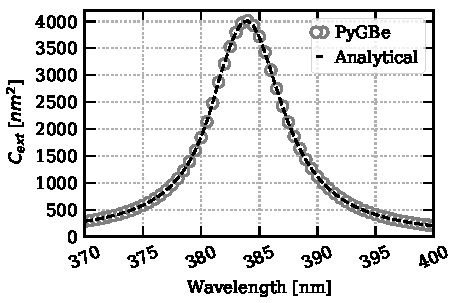
\includegraphics[width=0.85\textwidth]{silver_NP_verification.pdf} 
    \caption{Extinction cross-section as a function of wavelength for an $8$ nm
             silver sphere immersed in water. The peak in the values of 
             extinction cross-section corresponds to the plasmon resonance of the metallic 
             nanoparticle under the incoming electric field. Figure, plotting script and 
             auxiliary files available under \textsc{cc-by} \cite{ClementiETal2018d}.}
    \label{fig:verif_sph}
 \end{figure}

\begin{table}%[h]
    \centering
    \caption{\label{table:quadparams2} Verification: Gauss quadrature points; 
    $K$ and $K_{fine}$ are per element; $N_k $ is per element edge (semi-analytical integration). } 
    \begin{tabular}{l l}
    \hline%\toprule
     distant elements: & $K=4$ \\
     near-singular integrals:   & $ K_{fine}=19$ \\
     singular elements:  & $N_k =9$ \\
    \hline%\bottomrule
    \end{tabular}
\end{table}


\begin{table}%[h]
    \centering
    \caption{\label{table:treeparams2} Verification: treecode and solver parameters.} 
    \begin{tabular}{l l}
    \hline%\toprule
    treecode order of expansion: & $P=6$\\
    MAC                                         & $\theta=0.5$\\
    GMRES tolerance                    & $10^{-3}$\\
    \hline%\bottomrule
    \end{tabular}
\end{table}

\section{LSPR response to Bovine Serum Albumin} \label{chap:lspr_response_bsa}

Localized surface plasmon resonance (LSPR) biosensors detect target molecules
by tracking frequency shifts in the plasmon resonance of metallic nanoparticles
in the presence of analytes \cite{WilletsVandyune2007}. The chapter presents the 
modeling of LSPR biosensors using \pygbe, and we show how our boundary elements approach is 
suitable to model this phenomenon. We compute the extinction cross section 
of a silver nanosphere with bovine serum albumin (BSA) proteins (PDB code: 4FS5,
BSA dimmer) in different locations around it. We placed two BSA dimers opposite to each other 
in three configurations ($\pm z$, $\pm y$, and $\pm x$), as shown by figures \ref{fig:display_z} and \ref{fig:display_xy}.
As a point of comparison, experiments by Teichroeb and co-workers
\cite{TeichroebETal2008} find a coverage of $2\times 10^{12} \quad \text{molecules}/cm^2$ or $3.3\times 10^{12} \quad \text{molecules}/cm^2$, 
with a gold sphere 15-nm in diameter. In that work, the molecular size reported is 5.5 nm$\times$5.5 nm$\times$9 nm, resulting in
a number of attached molecules between 4 and 6. The BSA molecule used in our work corresponds to a dimer, i.e., approximately 
double the size of that in Teichroeb et al.'s experiment. With two BSA dimers in the proximity of the sensor, 
the volume fractions in the near-by region are comparable.


\subsection{Grid convergence analysis} \label{sec:grid_conv_bsa}
We perform a grid convergence study to ensure that the meshes are correctly
resolving the numerical solutions. We performed the convergence analysis of
the system sketched in in Figure \ref{fig:analyte-sensor}. Given that we 
compute the extinction cross section by integrating over the sphere, we set 
a fixed mesh density for the protein and refined the mesh of the nanosphere 
(512, 2048, 8192, 32768 elements). For the protein, we found that a mesh with
two triangles per $\text{\AA}^2$ was fine enough for the convergence 
analysis, resulting in $N_{prot} = 98116$ elements.
We use the same conditions used in the grid convergence analysis of the 
isolated nanoparticle of section \ref{sub_sec:grid_conv_iso}, presented
in Tables \ref{table:quadparams1} and \ref{table:treeparams1}. The protein 
dielectric constant for a wavelength of 380 nm is $2.7514 + 0.2860i$, this  
value was computed using a functional relationship provided by Phan
 et al.~\cite{PhanETal2013}. The protein was located at a distance of 
 $d=$ 1 nm of the sphere along the z-axis, such that its dipole moment 
 was aligned with the y-axis. We show the errors in Figure  \ref{fig:err_sph-bsa} 
 and table \ref{table:err_sph-bsa} which were computed using the Richardson extrapolated
\ref{sec:rich_extrapolation} value of the extinction cross section $C_{ext}= 1778.73$ nm$^2$.

\begin{figure}%[h] %  figure placement: here, top, bottom, or page
    \centering
    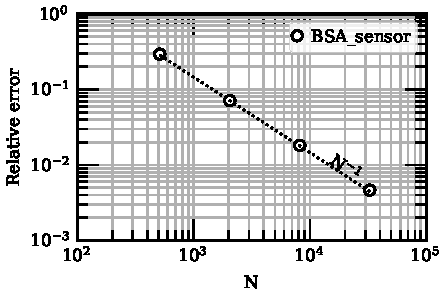
\includegraphics[width=0.85\textwidth]{convergence_bsa_sensor_R8_d1_w380.pdf} 
    \caption{Grid-convergence study of extinction cross-section of a spherical silver
             nanoparticle with a BSA protein at $d=1$ nm. 
             Figure, plotting script and auxiliary files available 
             under \textsc{cc-by} \cite{ClementiETal2018c}.}
    \label{fig:err_sph-bsa}
 \end{figure}

 \begin{table}%[h]
    \centering
    \caption{\label{table:err_sph-bsa} Estimated percentage error of the BSA-sensor 
    system (Fig.~\ref{fig:analyte-sensor}), with respect to the extrapolated value 
    (using Richardson extrapolation).} 
    \begin{tabular}{c c}
    \hline%\toprule
    N & \% error \\
    \hline%\midrule
     $512$ & $29.39$ \\
     $2048$ & $7.13$ \\
     $8192$ & $1.82$ \\
     $32768$ & $0.46$ \\
    \hline%\bottomrule
    \end{tabular}
\end{table}

The observed order of convergence is 0.99, and we can see in Figure
\ref{fig:err_sph-bsa} that the error decays with the number of boundary elements
at a rate of $1/N$, which is consistent with the verifications results showed
in Section \ref{sec:verification}. This shows that the numerical solutions computed
with \pygbe are correctly resolved by the meshes.

\subsection{Plasmon resonance frequency shifts} \label{sec:shift_bsa}

When a target molecule approaches the metallic nanoparticle, the resonance frequency
of this nanoparticle shifts. In this section, we computed the LSPR response as a
function of the wavelength in the presence of BSA protein. We optimized run times 
without compromising accuracy by using a relaxed set of parameters. For the protein
mesh density we used one element per $\text{\AA}^2$ ($N_{prot} = 45140$) and for the
sphere mesh we used $N_{sensor} = 32768$ elements. These calculations used the same
parameters from Tables \ref{table:quadparams2} and \ref{table:treeparams2}, which 
resulted in a percentage error below $1\%$, with respect to the Richardson-extrapolated
value. The run time for one frequency when two proteins are present, is approximately 
$15$ min using a NVIDIA Tesla K40c GPU.



\begin{center}
    \begin{figure} %  figure placement: here, top, bottom, or page
       \centering
       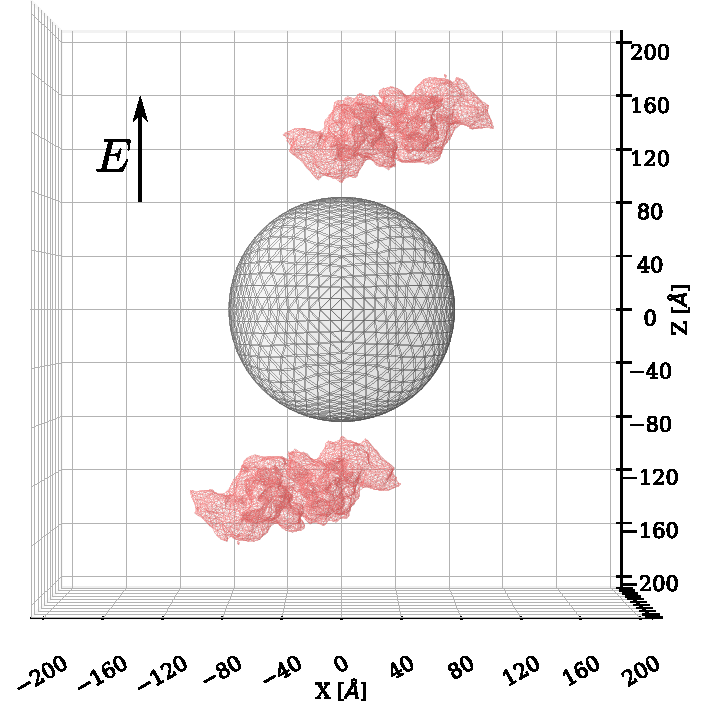
\includegraphics[width=0.85\textwidth]{2prot_1nm_z_R8nm.pdf} 
       \caption{Sensor protein display: BSA located at $\pm 1$ nm of the 
                nanoparticle in the $z$-direction. Figure, plotting script and auxiliary 
                files available under \textsc{cc-by} \cite{ClementiETal2018e}.}
       \label{fig:display_z}
    \end{figure}
    \end{center}

Figure \ref{fig:display_z} shows a visualization of the meshes setup for these 
calculations, with two BSA proteins located at $d=1$ nm away from the spherical 
silver nanoparticle, along the $z$ axis. The position of the BSA molecule at $+z$ 
axis was the same used for the convergence analysis in section \ref{sec:grid_conv_bsa},
while the protein located in the $-z$ position is a 180$^\circ$ solid rotation 
about the $y$ axis, of the BSA in $+z$.  Figure \ref{fig:2pz_response} shows the results
of the calculations between 382 and 387 nm every $0.25$ nm, near the peak seen in Figure
\ref{fig:verif_sph}. In Figure \ref{fig:2pz_response} we have the variation of the 
extinction cross section with respect to wavelength for the isolated nanoparticle 
($d=\infty$) and with BSA proteins located at $d=1$ nm apart from the nanosphere. The
result shows a redshift ($0.5$ nm) in the resonance frequency due to the presence of 
the BSA analytes.

\begin{figure} %[h] %  figure placement: here, top, bottom, or page
    \centering
    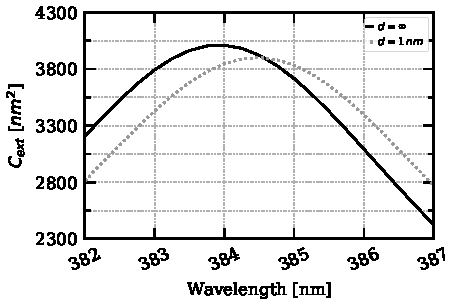
\includegraphics[width=0.85\textwidth]{2pz_R8nm.pdf} 
    \caption{Extinction cross-section as a function of wavelength for an $8$ nm
             silver sphere immersed in water with two BSA proteins placed 
             $\pm 1$ nm away from the surface in the $z$-direction, and at
             infinity (no protein).}
    \label{fig:2pz_response}
 \end{figure}

Figure \ref{fig:2pz_response} shows a redshift of the plasmon resonance frequency 
peak in the presence of two BSA proteins located at 1 nm along the $z$ axis. Experimental 
observations in the work of Tang, et al.~\cite{TangETal2010} revealed a redshift when 
BSA proteins in a solution are added to silver nanoparticles of approximately $17$ nm 
in diameter. They also observed a decrement of the peak amplitude, similarly to the 
effects we see with our model. Moreover, recent experiments \cite{PuETal2018} report 
resonance frequency between $380$ and $400$ nm for a silver nanosphere in the presence
of BSA proteins (check reference and its supplementary material), which is consistent with 
our results. Other experiments \cite{RaphaelETal2013} also report redshifts in the presence
of different proteins. The boundary element method approach that we implemented using 
electrostatic approximation is thus able to capture the characteristics of LSPR biosensors
based on resonance-frequency shift. 

We also study the effect of the location of the proteins, we performed the same 
calculations but now placing the BSA analytes along the $x$ and $y$ axis at $\pm 1$ nm,
as shown in Figure \ref{fig:display_xy}. We obtain these configurations by performing
a 90$^\circ$ solid rotation of the $z$-configuration (Figure \ref{fig:display_z})
along the $x$- and $y$-axis, respectively. Figure \ref{fig:2pxy_response} shows the 
results for each configuration.

 \begin{figure}
    \centering
    \subfloat{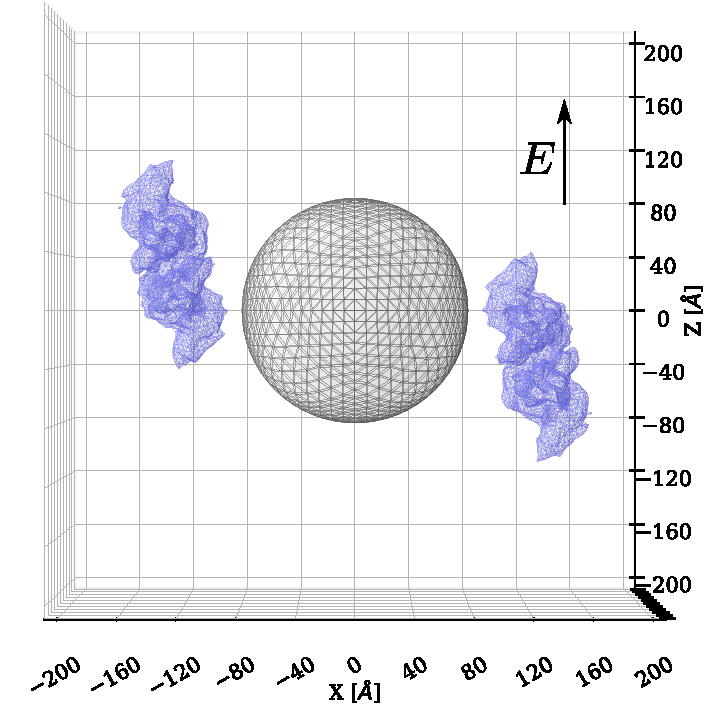
\includegraphics[width=0.65\textwidth]{2prot_1nm_x_R8nm.pdf}} \\
    \subfloat{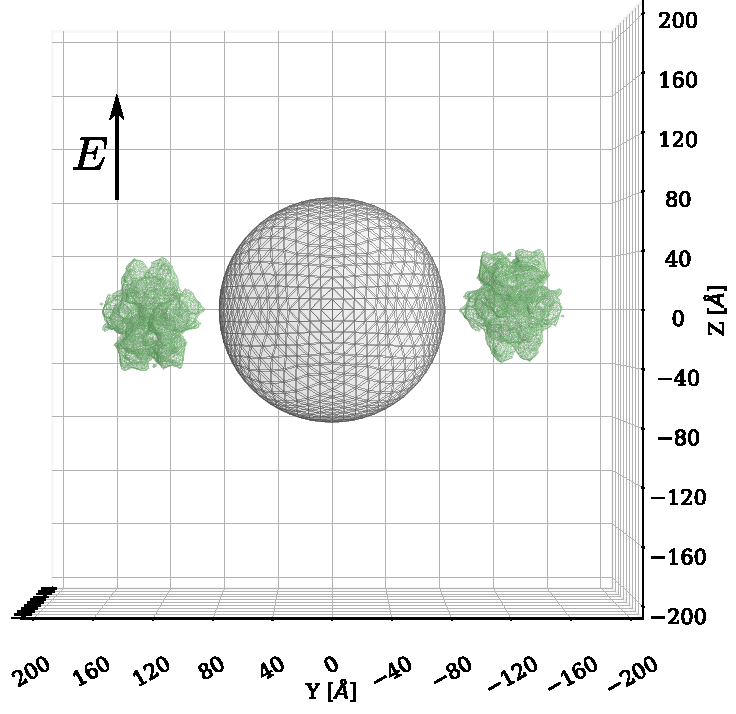
\includegraphics[width=0.65\textwidth]{2prot_1nm_y_R8nm.pdf}} 
     \caption{Sensor protein display: BSA located at $\pm 1$ nm of the nanoparticle in the
            $x$-direction (top) and $y$-direction (bottom). Figure, plotting script and 
            auxiliary files available under \textsc{cc-by} \cite{ClementiETal2018e}.}
     \label{fig:display_xy}
 \end{figure}

 \begin{figure}%[t] %  figure placement: here, top, bottom, or page
    \centering
    \subfloat{\includegraphics[width=0.85\textwidth]{{2px_R8nm}.pdf}}\\
    \subfloat{\includegraphics[width=0.85\textwidth]{{2py_R8nm}.pdf}} 
    \caption{Extinction cross-section as a function of wavelength for an $8$-nm
             silver sphere immersed in water with two BSA proteins placed at
             $\pm 1 $ nm away from the surface in the $x$-direction (top) and
             $y$-direction (bottom), and at infinity (no protein).}
    \label{fig:2pxy_response}
 \end{figure}

Figure \ref{fig:display_xy} shows the configuration where the proteins are placed at a 
distance in the $x$ (top) or $y$ (bottom) direction. For these configurations and with 
the electric field aligned with the $z$ axis, the LSPR response is negligible. The 
frequency shifts in Figure \ref{fig:2pxy_response} are smaller than the wavelength 
resolution ($<0.25$ nm). This finding is consistent with the free electrons oscillating
along the $z$ axis under a $z$-polarized electric field, and not in the $x$ and $y$ 
directions {\color{red} ADD REFERENCE TO FIG OF OSCILLATING ELECTRONS - LSPR}. The 
proteins have a marked effect when placed in the $z$ direction, where they can interfere 
with the oscillation of the free electrons. 

\subsection{Sensitivity study} \label{sec:sensitivity}

On LSPR biosensors we refer to sensitivity to the relationship between the size of the 
resonance frequency shift and the number of analytes bound to the sensor (through the 
ligand). Experiments show that the distance between the protein and the nanoparticle 
affects the sensitivity of the sensor, to the point that targets placed 15 nm away 
from the surface are hardly detectable \cite{HaesETal2004}. This is a critical issue
considering that most common ligands, like antibodies, can be larger than 15 nm. In 
Figure \ref{fig:dist_response} we can see how the resonance peak varies with the distance 
at which the  analytes are located ($+z$ and $-z$). When $d=2$ nm we have a shift of 
$0.25$ nm while when the analytes are at $d=0.5$ nm the shift is $0.75$ nm. The parameters
used in these simulations remain the same as the ones used for the cases in Figures 
\ref{fig:2pz_response} and \ref{fig:2pxy_response}.

\begin{figure}%[h] %  figure placement: here, top, bottom, or page
   \centering
   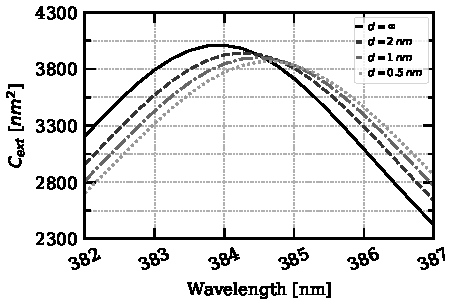
\includegraphics[width=0.85\textwidth]{2pz_lspr_response.pdf} 
   \caption{Extinction cross-section as a function of wavelength for an $8$-nm
            silver sphere immersed in water with two BSA proteins placed at
            $2$, $1$, and $0.5$ nm away from the surface in the 
            $z$-direction, and at infinity (no protein). The test case with
            $d=0.5$nm is close to the limit where quantum tunneling might happen. 
            Such effects are not captured by our classical model.}
   \label{fig:dist_response}
\end{figure}

As expected, Figure \ref{fig:dist_response} shows how the shift decreases as the BSA 
proteins move away from the nanoparticle, to the point that we only see a shift of 
$0.25$ nm when the analyte is $2$ nm away. This results shows the potential of \pygbe 
and the electrostatic approach to study biosensors sensitivity with distance. It's 
worth noting that quantum effects (e.g., tunneling) at $d=0.5$ nm are ignored with 
our classical approach. Even if this distance could be close to the quantum regime, 
there is evidence that classical theory is valid at this distance in similar systems
\cite{SavageETal2012, EstebanETal2012}

Even though there is evidence that techniques such as plasmon-enhanced Raman 
scattering are capable of detecting to the single-molecule limit 
\cite{ZhangZhangETal2013}, as far as we know there is no evidence of a purely
LSPR approach that can sense such low concentrations of proteins. Our 
computational results can unveil potential improvements that would enhance 
the sensitivity of LSPR biosensors, for example by using smaller ligands. 

There are not other LSPR simulations where the molecular details of the analyte 
are considered, that we are aware of. However, similar calculations can be 
performed with other open source softwares like BEM++ \cite{SmigajETal2015} and 
MATLAB toolbox MNPBEM \cite{HohenesterTrugler2012}. BEM++ also models the system
as a set of boundary integral equations, discretized in flat triangular panels, 
and it uses a Galerkin approach and algorithmic acceleration via hierarchical 
matrices. MNPBEM is another alternative software designed to simulate scattering
of metallic nanoparticles, which its BEM implementation is similar to \pygbe 
(centroid collocation with flat triangles) but with different acceleration scheme.
This MATLAB toolbox, similarly to BEM++, also relies on hierarchical matrices 
rather than a treecode, resulting in higher memory usage compared to our code, 
making it harder to simulate large analytes in detail. 
Commercial finite-element or finite-difference solvers can also be used for this
type of application, for example COMSOL. However, these volumetric approaches 
struggle to correctly impose the zero boundary condition at infinity, which is
exactly met for BEM.  

\section{Reproducibility and data management} \label{sec:repro_lspr}

All the results of this chapter have been published in the journal 
Physical Review E \cite{ClementiETal2019} and can be reproduced or replicated. \pygbe is openly developed and 
shared under the BSD3-clause license via its repository at \url{https://github.com/barbagroup/pygbe}.

All results of this chapter were obtained on a lab workstation, built from parts. Hardware specifications are as follows:

\begin{itemize}
  \item CPU: Intel Core i7-5930K Haswell-E 6-Core 3.5GHz LGA 2011-v3
  \item RAM: G.SKILL Ripjaws 4 series 32GB (4 x 8GB)
  \item GPU: Nvidia Tesla K40c (with 12 GB memory)
\end{itemize}

We release all of the data and scripts needed to run the calculations reported in this chapter, 
as well as the post-processing scripts to reproduce the figures. 
All the input files necessary to reproduce the computations are available in a Zenodo data set \cite{ClementiETal2018a}. 
Each folder contains the geometry files and charges files when applicable (.pqr), configuration files and parameter files.
We provide the scripts and any additional file needed to run \pygbe to re-generate every result in this chapter, in a 
separate Zenodo deposit \cite{ClementiETal2018b}. The execution of these scripts will generate the user's own version of the data needed to re-create 
the figures of this chapter (For more details, the reader can consult a \texttt{README} file in the Zenodo archive).
Finally we provide \emph{Reproducibility packages} deposited on Figshare to reproduce the figures in this chapter, which include 
figures, plotting scripts and Jupyter notebooks that organize and re-create the results 
\cite{ClementiETal2018c,ClementiETal2018d,ClementiETal2018e,ClementiETal2018f}.


%Next big section should be on Reduced order model for protein in LSPR applications
%Here we will put all the results of: pqr effect, ellipsoids effects, dielectric effect.
% !TEX root = ../thesis_main.tex
\chapter{Effects of a reduced order model for protein representation}
\graphicspath{{rom_studies/figs/}}

Part of the process of computational modelling is making assumptions about the problem we are trying to solve. In the 
field of localized surface plasmon resonance for biosensing applications there are several research papers that use Bovine Serum Albumin 
as an analyte to simulate the behavior of a bioconjugate sensor. However, they use extremely simplified models
to represent the protein, and often a real-valued dielectric for the medium. Some models consist of  
a layer of protein-water solution \cite{PhanETal2013}, 
or just a protein dielectric layer \cite{NghiemETal2012}, others model the
protein as a triangular prism \cite{DanHu2014}, or even a small sphere with a 
constant dielectric \cite{AntosiewiczApellClaudioKall2011, DavisGomezVernon2010,SantiagoCordobaETal2011, UngerETal2009}. Phan and 
coworkers \cite{PhanETal2013} present a Lorentz-Drude model for the complex 
dielectric of the BSA which we use in our work, while most of the literature 
use a constant dielectric with no losses to represent the BSA 
(refractive index of $n= 1.9$ \cite{NghiemETal2012}, $n= 1.45$ \cite{SantiagoCordobaETal2011}) or
other proteins used as analytes ($n=1.58$ polystrene \cite{UngerETal2009}, $n=1.57$ 
streptavidin \cite{ShenETal2013}). 

Research shows that the shape of both monomer and dimmer of BSA are prolate ellipsoids 
\cite{MoserETal1966, SquireETal1968, WrightETal1975}. However, we have not seen in the literature the use of ellipsoids 
to model the protein in computational approaches. The BSA model that we use, based on its crystal 
structure, is a good reference of the actual shape of the protein to be used as a comparison with simpler models. We 
explored the effects of using reduced-order models for the protein representation, like ellipsoids and spheres, and
studied the consequences of these simplifications. We analyzed the effects of the model chosen 
for the charges inside the protein (full distribution, monopole equivalent charge, and no charges), the protein orientation, the 
amount of proteins in the vicinity of the nanoparticle, the magnitude of the incident electric field, and the value and type (complex or real)
of the protein and water medium dielectrics. 

To the best of our knowledge, there is no model in the literature that accounts for the charges inside the protein. 
Moreover, there are no studies that explore the effects of using reduced-order models for the protein representations 
in computational models. This chapter covers the results of using different assumptions in the modelling process and their implications.

\section{BSA as a prolate ellipsoid} \label{sec:ell_study}

The crystal structure of the BSA (pdb 4f5s) used in our simulations corresponds
to a dimer. Knowing that this structure can be modeled as an ellipsoid \cite{SquireETal1968},
we look for different alternatives to decide the dimensions of the ellipsoid. We took two
different approaches, a surface equivalent model and a volume equivalent model. The surface equivalent
model consists of finding the dimensions of an ellipsoid that encapsulates all the charges within the protein. We determined the principal axes of this
ellipsoid using Principal Component Analysis (PCA). Principal component analysis is a technique that
uses orthogonal transformations and brings out patterns in a set of data. When 
we use a PCA in three dimensions, these transformations ensure that the first 
component is the one with most variation, the second one is the second-most, and
third one the least. This technique gives us the three eigenvectors that best 
describe the cloud of mesh-vertices. The values of the principal axis are $a=98.9\, \text{\AA}$, $b=54.2\, \text{\AA}$, and $c=41.8\, \text{\AA}$, and 
using these vectors when creating the mesh of the ellipsoid ensures that all the charges are contained.
In the second approach to model the BSA we create an ellipsoid that matches the volume of the BSA. To find the dimensions 
of the volume-equivalent ellipsoid we made some approximations. We obtained the volume of the BSA protein from the original mesh
using Trimesh (\url{https://github.com/mikedh/trimesh})), and looking at the PCA principal axis we noticed that $b$ and $c$ are close 
compared to $a$, and that $a$ is double the size. Then we can say that $b=c=x$ and $a=2x$, agreeing with the results from Squire and co-workers
\cite{SquireETal1968}. Using these approximations we can write the volume of the ellipsoid:

\begin{equation}
    V_e = \frac{4\pi}{3}a\,b\,c 
\end{equation}

as 

\begin{equation}
    V_e = \frac{4\pi}{3}2\,x^3
\end{equation}

Knowing that the volume of the BSA protein is $V_e = 166642 \, \text{\AA}^3$ we get that $x=27.09496 \, \text{\AA}$ 
and therefore $a=54.18993 \, \text{\AA}$ and $b=c=27.09496 \, \text{\AA}$. These dimensions give us an ellipsoid that has the same volume 
as the original BSA mesh. However, we can not encapsulates all the charges inside of it. To be able to use this model we needed to study first the 
effects of replacing the distribution of charges by a monopole, as well as the possibility of not including them in the model. 

All the ellipsoidal meshes were generated with a Python script that can be found in the code repository \url{https://github.com/pygbe/pygbe}. The
meshes for all the results in this chapter are provided as part of the reproducibility packages. Detailed information regarding this packages can be 
found in section \ref{sec:repro_ell}

\subsection{Effect of charges within the protein}

Since the PCA model can encapsulates all the charges we use this model to study the effect of using a distribution of charges, versus
a monopole representation of the charges ("center of mass"), as well as using no charges. To ensure that we are solving the equations 
properly, we perform a convergence analysis.

\subsubsection{PCA ellipsoid convergence analysis}

We performed a grid convergence analysis on the PCA (Principal Component Analysis) ellipsoid - sensor system containing a full pqr (see Figure \ref{fig:one_pca_sketch}). 
Since we compute the extinction cross section of the sensor (8 nm radius silver sphere), we set a fixed mesh density for the ellipsoid and refine 
the mesh of the sphere ($N=512, 2048, 8192, 32768$). We found that a mesh with $N=5120$ elements for the ellipsoid was fine enough for the convergence analysis.
We used the same physical conditions and parameters that were used for the BSA-nanoparticle convergence analysis presented in
\ref{sec:grid_conv_bsa}. Similarly to the BSA-sensor system, the distance between the sensor and the PCA-ellipsoid 
was $d=1$ nm, and the ellipsoid was oriented such that the dipole moment of the charges was aligned with the $y$-axis. 
Table \ref{table:err_sph-pca} shows the percentages error for the different meshes used in this study, which were 
obtained using the Richardson extrapolated value of the extinction cross section as a reference, $C_{ext} = 1432.6560$ nm$^2$. The observed order
of convergence is $0.99$, and Figure \ref{fig:err_sph-pca} shows that the error decays with the number of boundary elements ($1/N$). This provides
evidence that the numerical solutions computed with \pygbe are correctly resolved by the meshes.  

\begin{figure}%[h] %  figure placement: here, top, bottom, or page
    \centering
    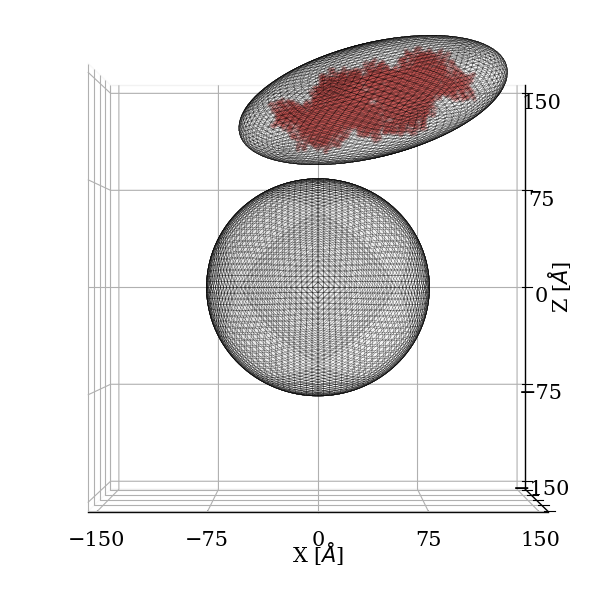
\includegraphics[width=0.65\textwidth]{viz/one_pca_full_display.png} 
    \caption{Sensor protein display: PCA ellipsoid with charges distribution located at $\pm 1$ nm of the 
    nanoparticle in the $z$-direction.}
    \label{fig:one_pca_sketch}
 \end{figure}


\begin{figure}%[h] %  figure placement: here, top, bottom, or page
    \centering
    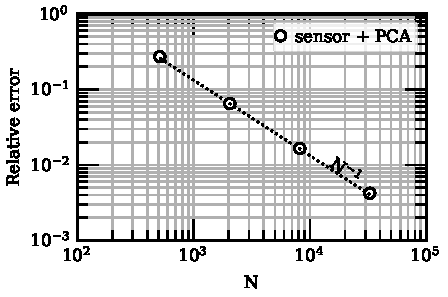
\includegraphics[width=0.85\textwidth]{convergence_sensor_pca_w380.pdf} 
    \caption{Grid-convergence study of extinction cross-section of a spherical silver
             nanoparticle with a PCA ellipsoid which contains 
             the charges distribution within it, located at $d=1$ nm.}
    \label{fig:err_sph-pca}
 \end{figure}

 \begin{table}%[h]
    \centering
    \caption{\label{table:err_sph-pca} Estimated percentage error of the PCA ellipsoid-sensor 
    system, with respect to the extrapolated value (using Richardson extrapolation).} 
    \begin{tabular}{c c}
    \hline%\toprule
    N & \% error \\
    \hline%\midrule
     $512$ & $27.2$ \\
     $2048$ & $6.5$ \\
     $8192$ & $1.66$ \\
     $32768$ & $0.42$ \\
    \hline%\bottomrule
    \end{tabular}
\end{table}

After performing the convergence analysis studies, we relaxed the numerical parameters of the computations to reduce the run-time without 
compromising accuracy. The following parameters were used to obtain all non-convergence results presented from now on for the case of PCA ellipsoids.

\begin{table}%[h]
    \centering
    \caption{\label{table:rel_pca_par} Relaxed parameters for the PCA ellipsoid case. The parameters that are not 
    mentioned here remain the same as in the convergence study.} 
    \begin{tabular}{c c}
    \hline%\toprule
    parameter & \% value \\
    \hline%\midrule
     $N_{sensor}$ & $8192$ \\
     $k_{fine}$ & $19$ \\
     $P$ & $6$ \\
     $tol$ & $1\times 10^{-3}$ \\
    \hline%\bottomrule
    \end{tabular}
\end{table}

The Richardson extrapolated value for the PCA case is: $1432.6561$ nm$^2$ and the computed value with the relaxed parameters 
is $1456.0781$ nm$^2$, giving us a percentage error of $1.63 \%$. 

\subsubsection{Charges model analysis} \label{ssub:pqr_analysis}

In order to know if we could use a volume equivalent (VE) approach we studied the effect of the charges inside the protein. We analyzed
the different representations of charges (full distribution and equivalent monopole), as well as the impact of having
no charges. The setup of the simulations consists of a silver sphere sensor ($r=8$ nm) with a PCA ellipsoid 
at $1$ nm of the surface of the sensor in the $z$-direction, oriented such that the dipole moment is aligned with the $y$-axis. We run 
three different cases, one with the full distribution of charges, a second case with one equivalent charge located in the
"center of mass" (See Figure \ref{fig:one_pca_cm_sketch}), and an ellipsoid with no charges. Figure 
\ref{fig:pqr_pca} shows the results for the different cases.

\begin{figure}%[h] %  figure placement: here, top, bottom, or page
    \centering
    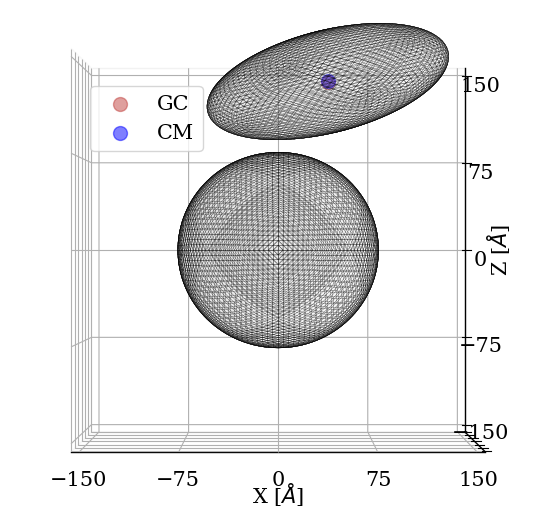
\includegraphics[width=0.65\textwidth]{viz/one_pca_cm_gc_display.png} 
    \caption{Sensor protein display: PCA ellipsoid with equivalent monopole charge, located at $\pm 1$ nm of the 
    nanoparticle in the $z$-direction. The label "CM" indicates the center of mass where the monopole charge is located, and
    the label "GC" indicates the geometric center for reference.}
    \label{fig:one_pca_cm_sketch}
 \end{figure}

 The resonance peak in all the curves in Figure \ref{fig:pqr_pca} occurs at $385.25$ nm. The 
 maximum value of the extinction cross section for the full distribution ("Full pqr") is $3827.06$ nm$^2$ and for 
 the monopole/center-of-mass representation ("CM pqr") is $3828.21$ nm$^2$, what results in a difference of $0.03 \,\%$. The
 maximum value of the extinction cross section when there are no charges present ("No pqr") is $3755.51$ nm$^2$ which compared to 
 the maximum for the full distribution gives us a difference of $1.87 \,\%$. Looking at these results we can say that the presence of 
 charges inside the protein does not affect the wavelength shift. However, it does affect the intensity of the maximum value of the 
 extinction cross section by approximately $2 \,\%$. Finally, we can say that using a monopole approximation for the distribution of charges, 
 is equivalent to using the full distribution of charges. Therefore, we will use the monopole charge model when doing computations with 
 a volume equivalent ellipsoid. 

\begin{figure}%[h] %  figure placement: here, top, bottom, or page
    \centering
    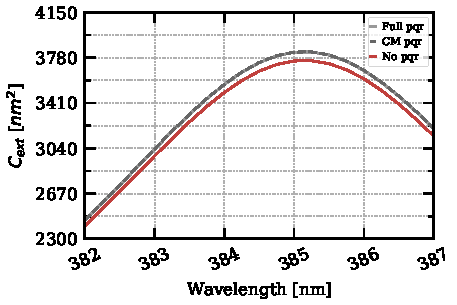
\includegraphics[width=0.85\textwidth]{pqr_analysis_pca.pdf} 
    \caption{Extinction cross-section as a function of wavelength for an $8$ nm
    silver sphere immersed in water with one PCA ellipsoid at $1$ nm away from 
    the surface in the $z$-direction, under a constant electric field on the $z$-direction.
    The label "Full pqr" corresponds to the full distribution of charges, the label "CM pqr" corresponds to a monopole representation 
    of the charges obtained by computing the center of mass of them, and the label "No pqr" 
    corresponds to the case where there are no charges present.}
    \label{fig:pqr_pca}
 \end{figure}



\subsection{Surface equivalent vs Volume equivalent model} \label{ssec:surf_vol_ell}

In section \ref{ssub:pqr_analysis} we show that using a monopole approximation is equivalent to using the full distribution of charges. This 
allows us to explore the effects of the volume equivalent model. Similarly to the PCA case, we present a convergence study for the volume  n section \ref{sssec:ve_conv}. 
Following the convergence study of the volume equivalent ellipsoid we show, in section \ref{sssec:ell_mod_comp}, the comparison of the PCA ellipsoid model and the volume equivalent 
model with the original BSA protein structure model, replicating the configuration shown in Figure \ref{fig:display_z}. 

\subsubsection{Volume Equivalent ellipsoid convergence analysis}\label{sssec:ve_conv}

We performed a grid convergence analysis on the VE (volume equivalent) ellipsoid - sensor system containing a monopole charge located 
in the center of mass of the charge distribution. (see Figure \ref{fig:one_ve_sketch}). Since we compute the extinction cross section of the sensor 
(8 nm radius silver sphere), we set a fixed mesh density for the ellipsoid and refine 
the mesh of the sphere ($N=512, 2048, 8192, 32768$). We found that a mesh with $N=1280$ elements for the ellipsoid was fine enough for the convergence study.
We used the same physical conditions and parameters that were used for the BSA-nanoparticle convergence analysis presented in
\ref{sec:grid_conv_bsa}. Similarly to the BSA-sensor system, the distance between the sensor and the VE-ellipsoid 
was $d=1$ nm, and the ellipsoid was oriented such that the dipole moment of the charges was aligned with the $y$-axis. To obtain the error 
estimate we used Richardson extrapolated value of the extinction cross section as a reference, $C_{ext} = 1683.8117$ nm$^2$. Table \ref{table:err_sph-ve} shows 
the percentages error for the different meshes used in this study. The observed order of convergence is $0.99$, and Figure \ref{fig:err_sph-ve} shows that the error decays 
with the number of boundary elements ($1/N$). This provides evidence that the numerical solutions computed with \pygbe are correctly resolved by the meshes.  

\begin{figure}%[h] %  figure placement: here, top, bottom, or page
    \centering
    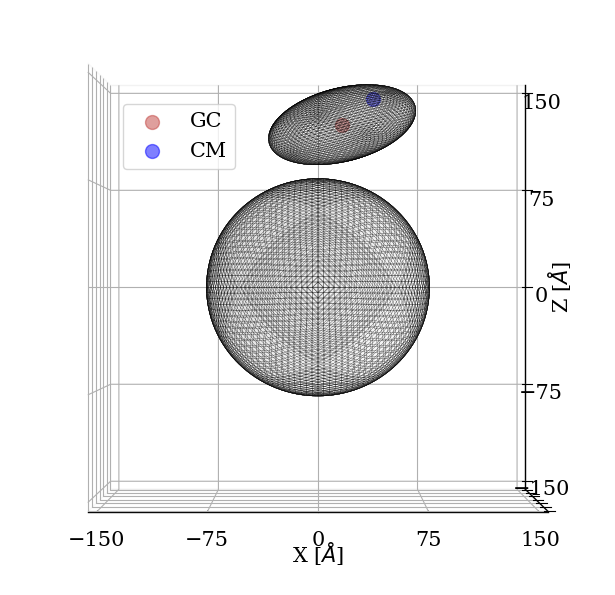
\includegraphics[width=0.65\textwidth]{viz/one_ve_cm_gc_display.png} 
    \caption{Sensor protein display: Volume equivalent ellipsoid with monopole charge ("CM"), located at $1$ nm of the 
    nanoparticle in the $z$-direction. The geometric center ("GC") is displayed for reference.}
    \label{fig:one_ve_sketch}
 \end{figure}


\begin{figure}%[h] %  figure placement: here, top, bottom, or page
    \centering
    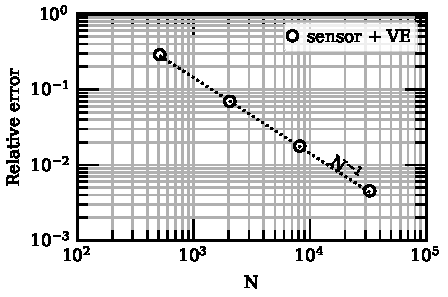
\includegraphics[width=0.85\textwidth]{convergence_sensor_ve_w380.pdf} 
    \caption{Grid-convergence study of extinction cross-section of a spherical silver
             nanoparticle with a volume equivalent ellipsoid at $d=1$ nm which contains 
             a monopole charge.}
    \label{fig:err_sph-ve}
 \end{figure}

 \begin{table}%[h]
    \centering
    \caption{\label{table:err_sph-ve} Estimated percentage error of the VE ellipsoid-sensor 
    system, with respect to the extrapolated value (using Richardson extrapolation).} 
    \begin{tabular}{c c}
    \hline%\toprule
    N & \% error \\
    \hline%\midrule
     $512$ & $28.8$ \\
     $2048$ & $6.96$ \\
     $8192$ & $1.78$ \\
     $32768$ & $0.45$ \\
    \hline%\bottomrule
    \end{tabular}
\end{table}

After performing the convergence analysis studies, we relaxed the numerical parameters of the computations to reduce the runtime without 
compromising accuracy. We use the parameters from Table \ref{table:rel_pca_par} to obtain all non-convergence results presented from 
now on for the case of VE ellipsoids. The Richardson extrapolated value for the VE case is: $1683.8117$ nm$^2$ and the computed value with 
the relaxed parameters is $1713.1972$ nm$^2$. If we compute the percentage error we obtain $1.75 \%$.

\subsubsection{Ellipsoid model vs original BSA}\label{sssec:ell_mod_comp}

In Figure \ref{fig:2pz_ell_resp} we show the results of comparing both ellipsoidal models of the protein with the 
original representation of the protein obtained from the crystal structure. We present the LSPR response 
of the system shown in Figure \ref{fig:display_z}, and for the ellipsoidal models we use an equivalent 
setup that replaces the proteins, located at $\pm 1$ nm in the $z$-direction, for the respective ellipsoids.
Both the PCA and VE model contain a monopole charge in the center of mass of the distribution. These results reveal 
the model chosen to represent the analytes matters.

\begin{figure} %[h] %  figure placement: here, top, bottom, or page
    \centering
    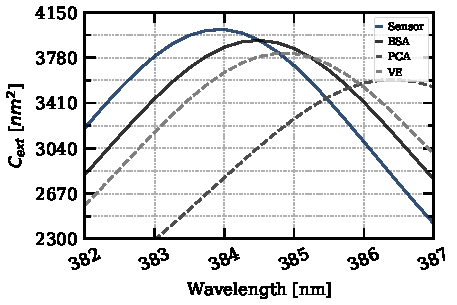
\includegraphics[width=0.85\textwidth]{two_ell_analysis.pdf} 
    \caption{Extinction cross-section as a function of wavelength for a 8 nm silver sphere immersed 
    in water with two BSA proteins ("BSA"), two PCA-ellipsoids with one equivalent charge ("PCA"), and two
    volume equivalent ellipsoids ("VE") with one equivalent charge. In all cases the proteins or equivalents
    are placed at $\pm 1$ nm away from the surface in the $z$-direction, except for the case where there is 
    no protein ("Sensor").}
    \label{fig:2pz_ell_resp}
 \end{figure}

The PCA model (surface based model, surface of PCA is $1.14$ times the original surface) over estimates the LSPR response, 
with a shift of $2.5$ nm ($400\%$ more) than the original shift ($0.5$ nm). The VE model (volume based based)  
overestimates the original by $50\%$ (shift $0.75$ nm), but we can say that a reduced order model based on the volume 
is a closer representation of the full protein. In both cases we see that the intensity of the peak decreases. This can be 
a problem, along with the overestimation of the shift, if the results are intended for use in the computation of sensitivity. The Figure of
Merit is usually how a nanoparticle's sensing capabilities are characterized, and is defined as the ratio between the 
sensitivity ($S = \Delta \lambda / \Delta n$) over the full width mid height (FWMH) \cite{otte2012}. Making 
conclusions of sensitive capabilities of sensors, based on models that underestimate the magnitude of the peak and 
overestimate the shift, can lead to incorrect assessments.

In summary, using an ellipsoidal shape of equivalent surface that contains all charges is not a good approximation
since it overestimates the shift considerably. The VE-equivalent model exhibits a shift of $0.75$ nm, which is still  
an overestimated response. However, we believe that the volume equivalent approximation can be used to investigate 
qualitative behaviors and take advantage of less expensive simulations to get insights on the physics of problems 
that might be impossible to simulate due to memory restrictions.

\subsection{Other model considerations}

Besides the effect of the surface and the volume based model as an approximation of the protein, there are other
factors that can affect the behavior of the system sensor-BSA. In this section we present the results of choosing a spherical 
geometry instead of an ellipsoidal model, the results of the protein orientation, the number of proteins in the vicinity of the nanoparticle, and 
the effect of the magnitude of the incident electric field. 

\subsubsection{Sphere vs Ellipsoid for protein modeling}

Spheres are one of the most common geometries used to represent the protein \cite{SantiagoCordobaETal2011, UngerETal2009}. In this 
section we compare a spherical volume-equivalent model with the ellipsoidal volume-equivalent model used in section
\ref{ssec:surf_vol_ell}. Figure \ref{fig:sph_vs_ell_ve} shows the different LSPR responses of a silver nanoparticle of $8$ nm of radius, 
for the different models. The peak for both the ellipsoid and the sphere of equivalent volume, happens at $384.75$ nm, and the 
maximum extinction cross section is nearly the same for both cases (difference $<$0.5$\%$). For the sphere simulation, 
the monopole charge was located at the geometric center. It is worth mentioning that locating the monopole charge in the
geometric center instead of the center of mass, has no impact on the LSPR response. We run simulations of a volume-equivalent ellipsoid 
with the charge on the geometric center and resulted in no variation of the resonance. The difference between the intensities at 
the peak is $<1\%$ (computations results in reproducibility materials, section \ref{sec:repro_ell}).

\begin{figure} %[h] %  figure placement: here, top, bottom, or page
    \centering
    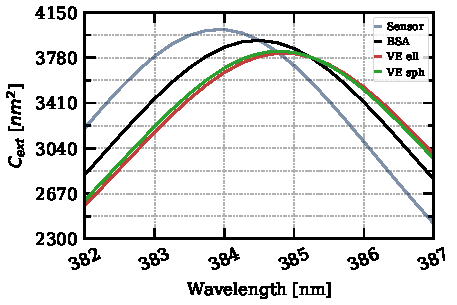
\includegraphics[width=0.85\textwidth]{two_ve_ell_sph_vs_BSA.pdf} 
    \caption{Extinction cross-section as a function of wavelength for an $8$ nm
    silver sphere immersed in water, under a constant electric field, with two volume equivalent 
    ellipsoids/spheres placed $\pm 1$ nm away from the surface in the $z$-direction.}
    \label{fig:sph_vs_ell_ve}
 \end{figure}

We still have the problem of overestimating the shift by $50$ $\%$ compared to the BSA protein original mesh, 
and at first sight we can consider this model comparable to the ellipsoidal volume-equivalent one. However, 
when we use a spherical model for the protein we lose any information regarding the orientation of the protein. 

\subsubsection{Effect of protein orientation}

Until this point we always kept the orientation of the proteins such that the dipole moment was parallel to the $y$-axis. In this 
section we explore the effects of protein orientation in respect to the nanoparticle in the LSPR response. For this study we use the 
volume equivalent ellipsoids in three different orientations: the original configuration where the dipole moment is parallel to 
the $y$-axis, a configuration such that the principal axis $a$ is parallel to $y$-axis, 
and finally a configuration where the principal axis $b$ is parallel to $y$ (see Figure \ref{fig:two_ve_conf_display} for configurations). 
 
 \begin{figure} %[h] %  figure placement: here, top, bottom, or page
    \centering
    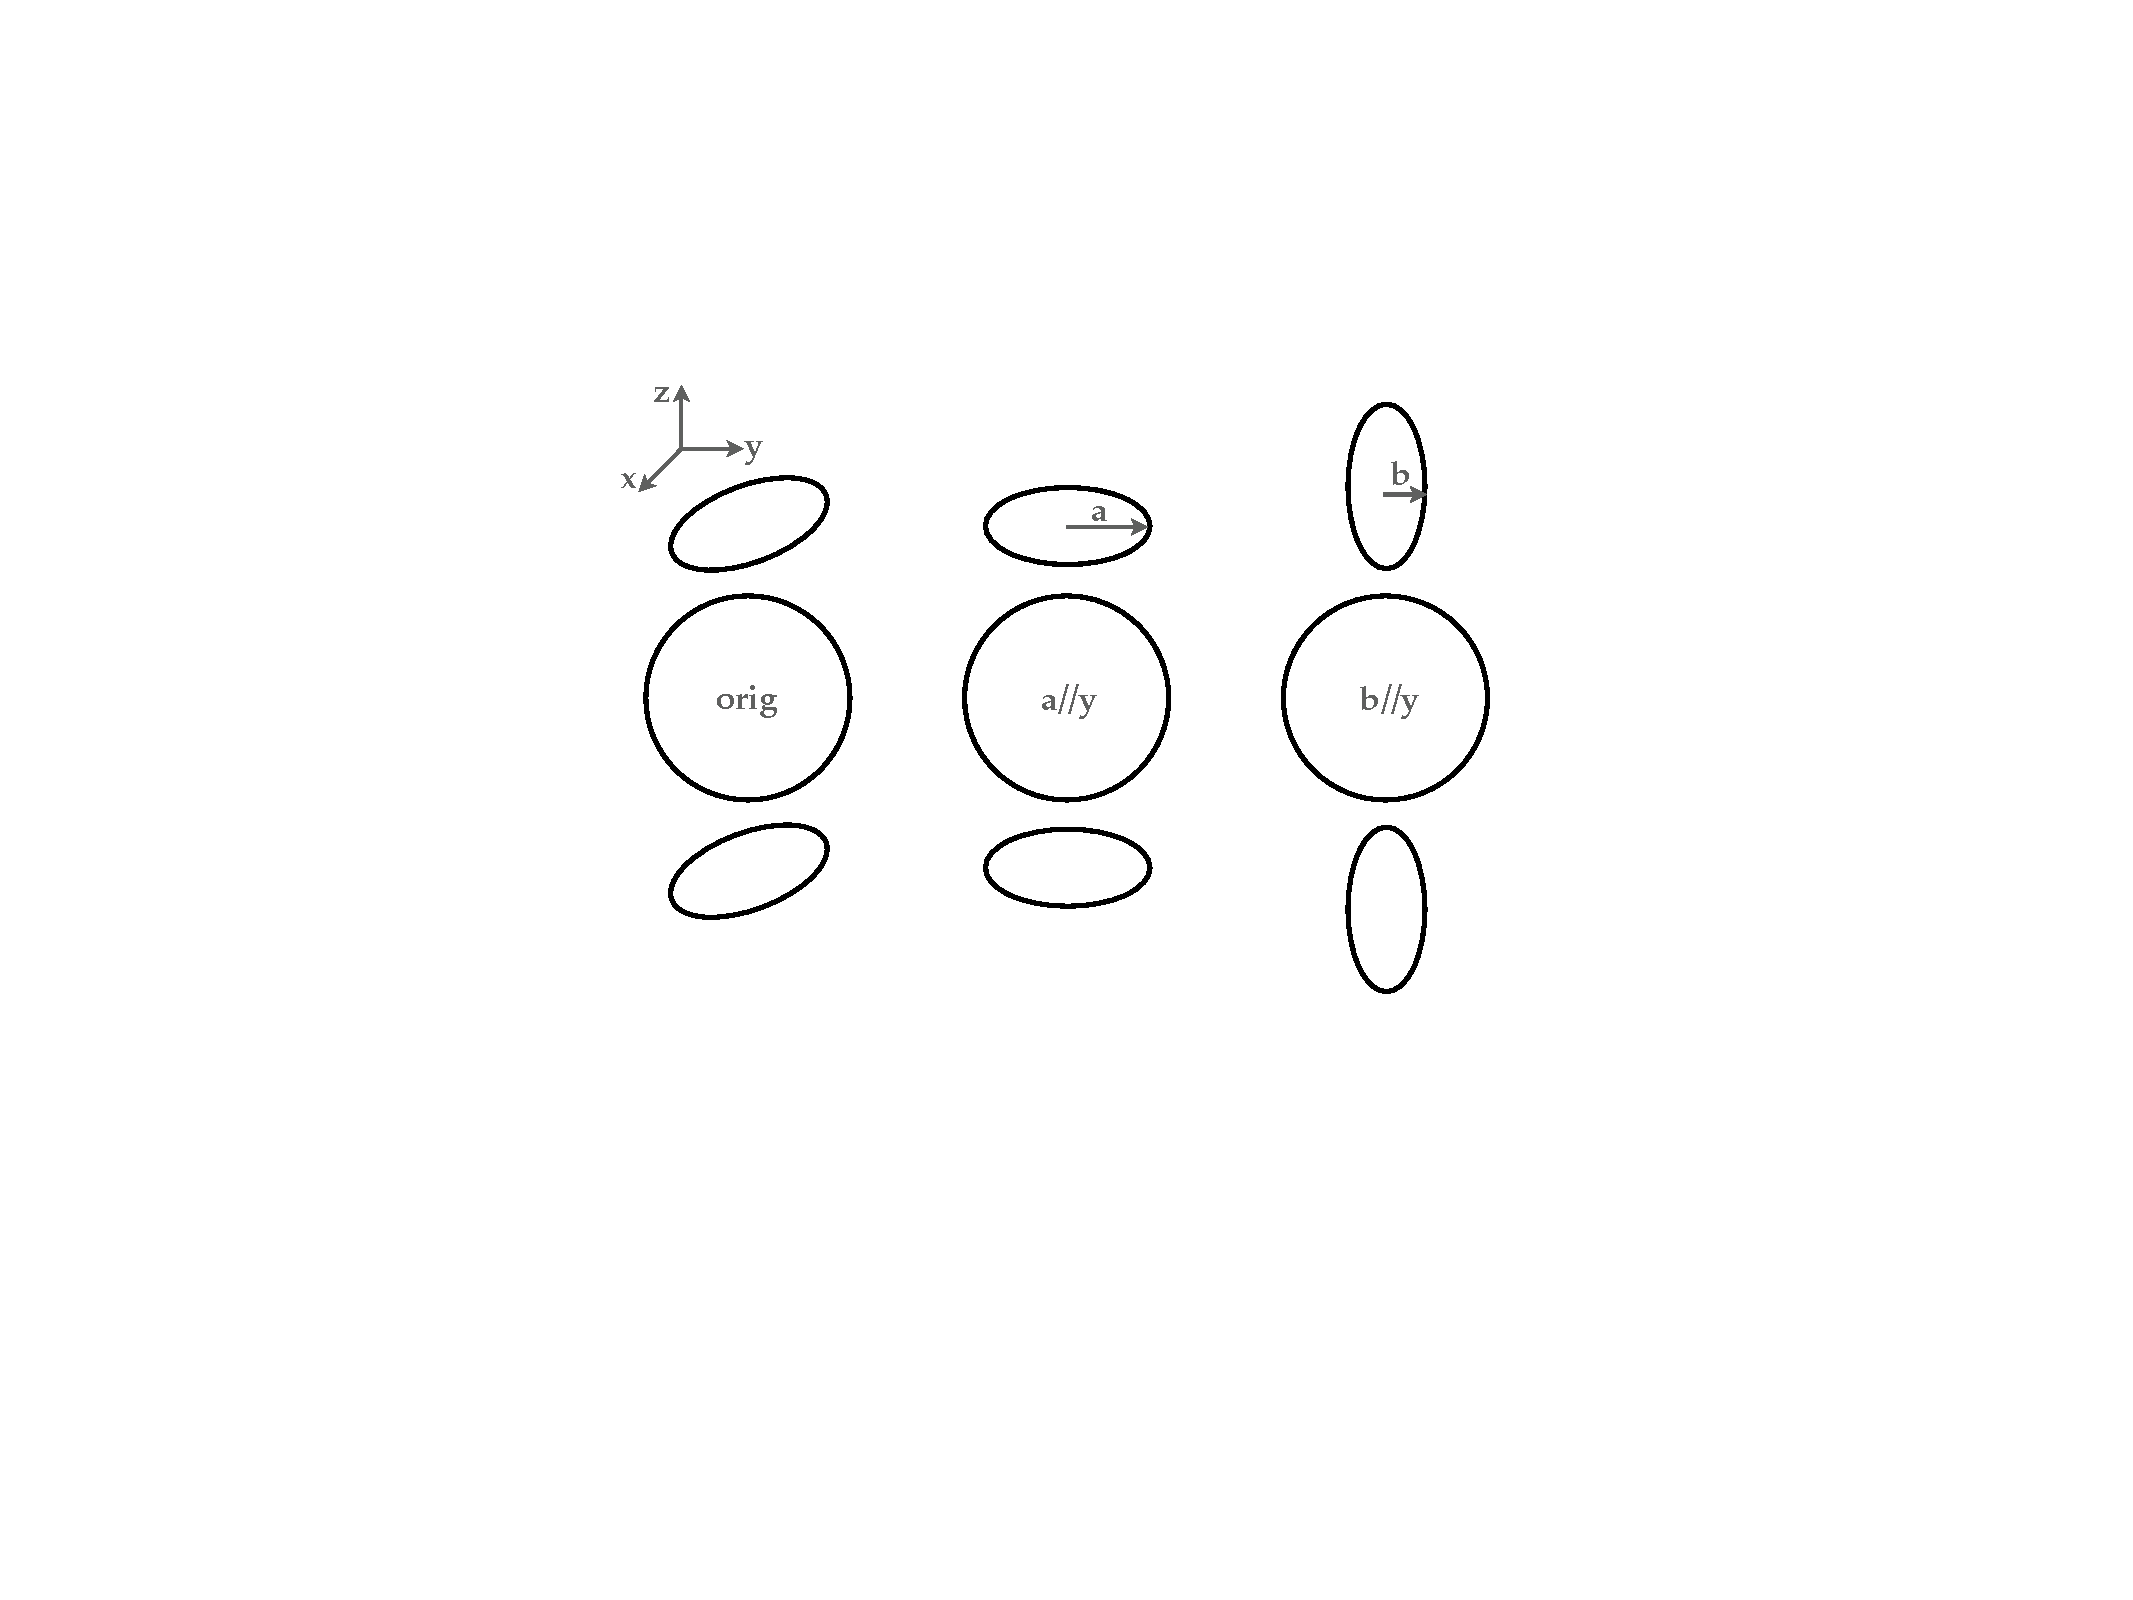
\includegraphics[width=0.65\textwidth]{viz/two_ve_conf_display.pdf} 
    \caption{Different configurations for two volume equivalent ellipsoids.}
    \label{fig:two_ve_conf_display}
 \end{figure}
 
 \begin{figure} %[h] %  figure placement: here, top, bottom, or page
     \centering
     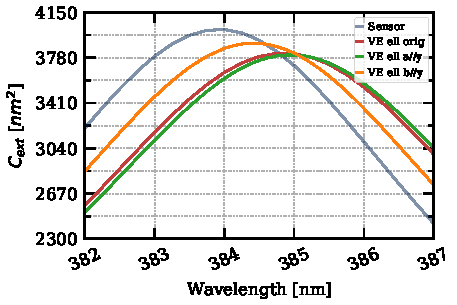
\includegraphics[width=0.85\textwidth]{two_ve_ell_mult_config.pdf} 
     \caption{Extinction cross-section as a function of wavelength for an $8$ nm
     silver sphere immersed in water, under a constant electric field, with two BSA ellipsoids placed 
     $\pm 1$ nm away from the surface in the $z$-direction. "VE ell orig": dipole moment parallel to the $y$-axis,
     "VE ell a//y": principal axis $a$ is parallel to $y$-axis, and "VE ell b//y": principal axis $b$ is parallel to $y$-axis}
     \label{fig:two_ell_mult_config}
  \end{figure}
 
Figure \ref{fig:two_ell_mult_config} shows the LSPR response of a silver nanoparticle when ellipsoids 
are placed in different positions and orientations. The peak when the dipole moment is parallel to the $y$-axis (original)
is $3815.72$ $nm^2$ and occurs at $384.75$ nm, causing a shift of $0.75$ nm. When the orientation of the ellipsoid 
is such that $a//y$, the maximum value is $3802.51$ $nm^2$ and it happens at $385$ nm, which results in a shift of 
$1$ nm. The final orientation we study is when $b//y$ which has a peak of $3898.10$ $nm^2$ at $384.375$ nm, resulting 
in a shift of $0.375$ nm. These results tell us that the orientation of the protein affects the LSPR response, we can 
see that the shifts vary depending on the orientation, as well as the intensity of the peak. When using a spherical model, 
all these effects are not captured due to the nature of the geometry, which can lead to misleading conclusions. Even though, 
we know that using a volume equivalent ellipsoid model overestimates the shift, it stills captures the effect of the orientation, making
it a better candidate compared to a simple sphere.

\subsubsection{Effect of number of proteins}

In this section we study the effect of having multiple proteins around the nanoparticle. Even though we know 
that volume equivalent ellipsoids overestimate the response, they still account for the effects of 
orientation and they can give us an estimation on how the LSPR response changes when having multiple 
ellipsoids. We use the same orientations shown in Figure \ref{fig:two_ve_conf_display} but we added ellipsoids 
at $\pm 1$ nm in the $x$ and $y$ directions too. Figure \ref{fig:mult_ell} shows the results of the LSPR response 
of six ellipsoids located at $\pm 1$ nm in the $x$, $y$, and $z$-axis, for the different configurations. 
 
\begin{figure} %[h] %  figure placement: here, top, bottom, or page
    \centering
    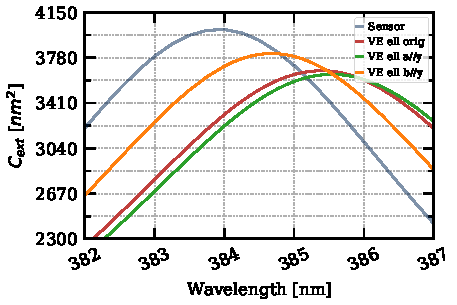
\includegraphics[width=0.85\textwidth]{six_ve_ell_mult_config.pdf} 
    \caption{Extinction cross-section as a function of wavelength for an $8$ nm
            silver sphere immersed in water, under a constant electric field, with multiple ellipsoids in different orientations 
            located at $\pm 1$ nm of the nanoparticle in the $x$, $y$ and $z$-axis.}
    \label{fig:mult_ell}
 \end{figure}

 The peak when the dipole moment is parallel to the $y$-axis (original) is $3673.89$ $nm^2$ and occurs at $385.375$ nm, causing a shift of 
 $1.375$ nm. When the orientation of the ellipsoid is such that $a//y$, the maximum value is $3643.97$ $nm^2$ and it
 happens at $385.5$ nm, which results in a shift of $1.5$ nm. The final orientation we study is when $b//y$ which 
 has a peak of $3814.23$ $nm^2$ at $384.625$ nm, resulting in a shift of $0.625$ nm. We can see that adding more proteins, 
 regardless of the orientation, increases the shift. However, depending on the orientation, the percentage of shift increment 
 varies. When we go from two ellipsoids on $\pm 1$ nm on the $z$-direction to six ellipsoids located at 
 $\pm 1$ nm in the $x$, $y$, and $z$-axis we see an increment on the shift of:
 
 \begin{itemize}
     \item {$~83\%$ when the dipole moment is parallel to the $y$-axis}
     \item {$50\%$ when the principal axis $a$ is parallel to the $y$-axis}
     \item {$~66.67\%$ when the principal axis $b$ is parallel to the $y$-axis}
 \end{itemize}    

These results tell us that the LSPR response is not only affected by the orientations but also by the number of proteins 
in the vicinity of the sensor. The addition of proteins, even though it always translates in a bigger shift, the increment  
is not linear, and it varies with the orientation. 

\subsubsection{Effect of magnitude of electric field}

Another factor that is involved in the computational model is the effect of the magnitude 
of the incident electric field. For all the simulations of this work we used the magnitude of the electric field from Phan and 
coworkers \cite{PhanETal2013}. In this section, we vary the magnitude of the electric field across several orders of magnitude 
and study its effect on the LSPR response. 

\begin{figure}%[t] %  figure placement: here, top, bottom, or page
    \centering
    \subfloat{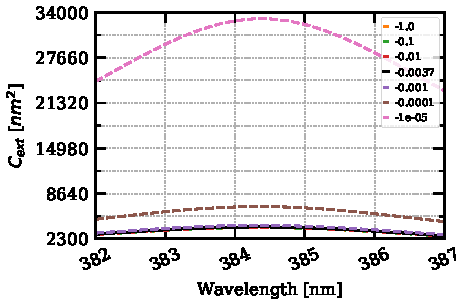
\includegraphics[width=0.85\textwidth]{VE_ell_cm_elec_field_var.pdf}}\\
    \subfloat{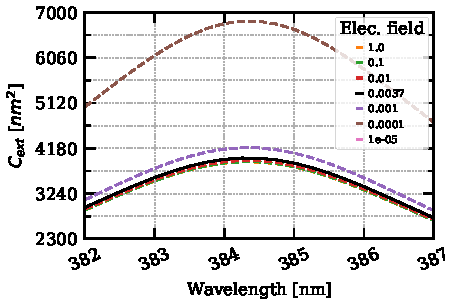
\includegraphics[width=0.85\textwidth]{VE_ell_cm_elec_field_var_zoom.pdf}} 
    \caption{Extinction cross-section as a function of wavelength for an $8$ nm
    silver sphere immersed in water, under a constant electric field, with a volume equivalent ellipsoid
    located at $1$ nm in the $z$-direction. The different colors represent different magnitudes of the 
    electric field where the units are $[e]/([{\text{\AA}}^2][\epsilon_0])$. The bottom figure is a zoom of the top 
    figure.}
    \label{fig:efield_effect}
 \end{figure}

Figure \ref{fig:efield_effect} shows how the magnitude of the incident electric field affects the LSPR response 
of a silver nanoparticle of radius $r=8$ nm when having a volume equivalent ellipsoid located 
$\pm 1$ nm in the $z$-direction (display Figure \ref{fig:one_ve_sketch}). We can see that as we decrease the magnitude of the electric field, 
the intensity of the extinction cross section increases. For all the different values of electric field except 
$1\times10^{-5}$ the peak occurs at $384.25$ nm, when the magnitude is $1\times10^{-5}$ the peak occurs at 
$384.5$ nm. This tells us that the magnitude of the electric field affects the shift. We computed 
the magnitude of the electric field due to the single charge inside the ellipsoid, on the surface of the nanoparticle,
and we found that its magnitude is $~5.4 \times 10^{-4}$ $[e]/([{\text{\AA}}^2][\epsilon_0])$. Therefore, 
when the magnitude of the incident electric field is smaller than the magnitude of the electric field generated by 
the protein on the surface of the nanoparticle, the shift increases. It is worth mentioning that if there are no charges 
present in the protein, the extinction cross section does not vary when the magnitude of the incident electric field 
changes. 


\section{Dielectric study}\label{sec:diel_study}

Most computational works in the literature use a constant real dielectric value both for the protein and the
embedding medium \cite{NghiemETal2012, SantiagoCordobaETal2011,UngerETal2009}. Such modeling does not account for the losses 
in that medium. LSPR biosensors detect a target molecule by monitoring plasmon resonance frequency changes due to the proximity 
of the target to the metallic nanoparticle. In this section, we show how the LSPR response changes when choosing different models 
for the dielectric in the protein and the medium around the system sensor-protein. We use the same setup used in chapter \ref{sec:lspr_response_bsa}
where we have two BSA proteins located at $\pm$ 1 nm on the $z$-direction of a silver nanoparticle of radius $r=8$ nm (see 
Figure \ref{fig:display_z}). The system sensor-protein is submerged in water and under a constant electric field of 
$0.0037$ $[e]/([{\text{\AA}}^2][\epsilon_0])$ in the $z$-direction. We first study the effect of having a real-valued dielectric 
for the protein, by keeping the water dielectric as complex. Second, we analyze the effect of the medium by using a real-valued 
dielectric, but we keep the BSA dielectric complex. Finally, we study the effect of certain combinations where both the medium 
and the protein have real-valued dielectrics. We obtained the values for the real dielectric of the BSA and water (medium) from the literature.
In most of the cases they provided the refractive index $n$, which we convert to the real dielectric $e_r=n^2$:  

\paragraph{BSA dielectric values:}
\begin{itemize}
    \item {Nghiem et al 2012 \cite{NghiemETal2012}: $n=1.9$, $e_r = n^2 = 3.61$}
    \item {Santiago-Cordoba et al 2011 \cite{SantiagoCordobaETal2011}: $n=1.45$, $e_r = n^2 = 2.0125$}
    \item {Phan et al 2013 \cite{PhanETal2013}: Average of real values of complex Lorentz-Drude model $e_r = 2.7498$}
\end{itemize}

\paragraph{Water dielectric values:}
\begin{itemize}
    \item {Real dielectric of water at room temperature $n=1.33$, $e_r = n^2 = 1.7689$}
    \item {Hale and Querry 1972 \cite{HaleQuerry1972}: Average of experimental real values $e_r = 1.7962$}
\end{itemize}
  
\subsection{BSA with real dielectric}

We study the effect of using a real-valued dielectric for the BSA, while keeping a complex-valued dielectric for the water where  
the system protein-sensor is embedded. Figure \ref{fig:bsa_diel} shows the extinction cross-section of silver nanoparticle 
of radius $r=8$ nm when having two BSA proteins located at $\pm1$ nm in the $z$-direction, for different dielectric models for the BSA. 
The computation of the original curve ("Complex") uses the complex dielectric for each frequency obtained from the Lorentz-Drude model 
from Phan et al. \cite{PhanETal2013}. The remaining curves correspond to the real-valued models from Santiago-Cordoba et al.\cite{SantiagoCordobaETal2011},
Nghiem et al \cite{NghiemETal2012}, and the average value of the real component from Phan et al. \cite{PhanETal2013}. The peak of the extinction cross section 
for both the complex model from Phan work \cite{PhanETal2013} and the average of its real part happen at $384.5$ nm, which represents a shift of $0.5$ nm from 
the LSRP response of the isolated nanoparticle. However, the intensity of the peak goes from $3901.06$ nm$^2$ to $4063.95$ nm$^2$ which is approximately a $~4.2\%$ increment. 
The resonance peaks for the values from Nghiem et al. and Santiago-Cordoba et al. occur at wavelengths $384.75$ nm and $384$ nm, respectively. These results 
translate in no shift for the case of Santiago-Cordoba et al., and a shift of $0.75$ nm for the case of Nghiem et al. The intensity for these two cases is 
bigger than the case where we used a complex dielectric for the model. 

\begin{figure} %[h] %  figure placement: here, top, bottom, or page
    \centering
    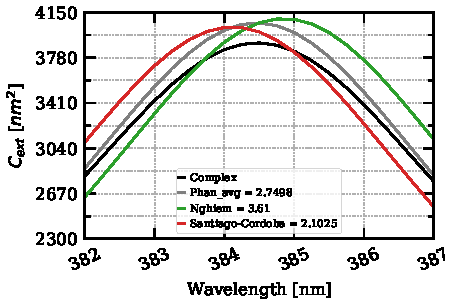
\includegraphics[width=0.85\textwidth]{bsa_diel_study.pdf} 
    \caption{Comparison of LSPR response of a silver nanoparticle to two BSA proteins located at $\pm1$ nm on the $z$-direction
    when using a complex vs a real dielectric for the protein.}
    \label{fig:bsa_diel}
 \end{figure}

The results from Figure \ref{fig:bsa_diel}, tell us that using a real dielectric for the protein affects the intensity of the extinction cross section. Using 
different values for the real dielectric also affects the LSPR response in terms of the shift. However, when comparing the complex model from Phan et al. versus
an average of the real parts of the dielectric, we see that the shift does not change. 

\subsection{Water with real dielectric}

After studying the effect of the dielectric model used inside the protein we explored the effects of the dielectric model in the 
embedding medium. We analyzed the effect of using a real-valued dielectric in the water when having the isolated nanoparticle (\ref{fig:iso_NP_diel}), 
as well as having the nanoparticle with two BSA proteins located at $\pm1$ nm on the $z$-direction (\ref{fig:real_w_comp_bsa}). We used
the complex dielectric values obtained from Hale and Querry \cite{HaleQuerry1972}, the average value of the real part from their work, and the real 
dielectric value for water at room temperature commonly used in the literature ("Generalization"). Figure \ref{fig:iso_NP_diel} shows
that using a complex representation of the dielectric versus using the average across the wavelengths of its real part, is indistinct. We can see that the curves
for the complex dielectric case (black curve) and the curve with average of the real part of the complex dielectric (green curve), match perfectly. However, when we
change the value of the real dielectric by a small amount (difference of $0.0273$), this has a big impact on where the peak occurs. For the "Generalization" case, where 
the dielectric is $1.7689$ we see that the peak occurs at a wavelength of $382.75$ nm, compared to the original peak for a dielectric of $1.7962$ which happens at $384$ nm. This shows
how sensitive is the LSPR response of the silver nanoparticle to the dielectric in which it is embedded. 
 
\begin{figure} %[h] %  figure placement: here, top, bottom, or page
    \centering
    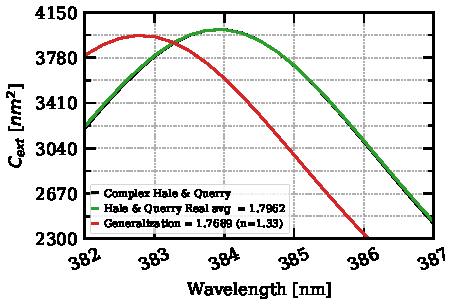
\includegraphics[width=0.85\textwidth]{iso_np_water_diel_study.pdf} 
    \caption{Comparison of LSPR response of isolated silver nanoparticle when using a complex 
     vs a real dielectric model for the water medium}
    \label{fig:iso_NP_diel}
 \end{figure}

Now that we understand how the dielectric model affects the LSPR response of the isolated nanoparticle, we can see how this 
effect varies when adding the BSA proteins at $\pm1$ nm on the $z$-direction. To isolate the effect of the dielectric model on the 
medium, we use the complex dielectric from Phan et al. \cite{PhanETal2013} for the BSA proteins. Figure \ref{fig:real_w_comp_bsa}
shows the shift in the LSPR response of a silver nanoparticle (dashed lines) when adding the BSA proteins (full lines), for the same 
real dielectrics models used in Figure \ref{fig:iso_NP_diel}. When using the average of the real part of the complex dielectric from 
Hale and Querry \cite{HaleQuerry1972} the shift is $0.5$ nm which is the same value compared to the full complex model. However, when using 
the generalization of the water dielectric (refractive index $n=1.33$), the peak for the extinction cross section when the two BSA proteins are
present occurs at a wavelength of $383.5$ nm, which gives us a shift in the LSPR response of $0.75$ nm. These results tell us that there is no 
difference in the LSPR response, wether we use the complex dielectric for the water or an averaged value of its real component. However, when using a
different real value for the dielectric, like the generalization $e=1.7689$, it not only affects the wavelength at which the resonance peaks occur
but also the shift when proteins are added in the vicinity. 

 \begin{figure} %[h] %  figure placement: here, top, bottom, or page
    \centering
    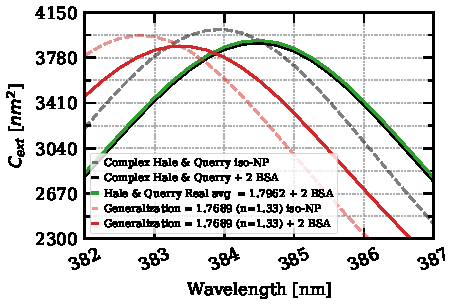
\includegraphics[width=0.85\textwidth]{bsa_w_real_water_diel.pdf} 
    \caption{Comparison of LSPR response of a silver nanoparticle to two BSA proteins located at $\pm1$ nm on the $z$-direction
    when using a complex vs real dielectric for the water medium.}
    \label{fig:real_w_comp_bsa}
 \end{figure}

 \subsection{BSA and water with real-valued dielectric}

Last but not least, we study the effect of using real-valued dielectrics for the BSA proteins as well as the water medium. For the BSA proteins 
we used the average value of the real component from Phan et al. \cite{PhanETal2013}, and for the water medium we used the same two dielectrics cases
used in the study of Figure \ref{fig:real_w_comp_bsa}. Figure \ref{fig:bsa_w_real} shows the results of using real dielectrics in both the proteins and
the water medium. The peaks in all cases occur at the same wavelengths compared to the case where we use a BSA complex dielectric for the protein, and as a 
consequence the shifts are the same than the ones reported in Figure \ref{fig:real_w_comp_bsa}. However, when we use real dielectric in both the medium 
and the proteins we see an increment in the magnitude of the extinction cross section of $~4.2\%$ for the Hale and Querry case, and $~3.6\%$ for the 
generalization case. These results tell us that, when it comes to the shift in the LSPR response, there is no difference between using a complex dielectric 
value for the protein and the medium, and using an averaged value of their real component. However, there is a difference in the magnitude of the 
extinction cross section that is a direct consequence of using a real-valued dielectric since this does not accounts for the losses in the medium. Similarly to the 
results shown in Figure \ref{fig:real_w_comp_bsa}, the usage of a different real dielectric for the water medium, changes where the peak occurs and the shift in the 
LSPR response. 

 \begin{figure} %[h] %  figure placement: here, top, bottom, or page
    \centering
    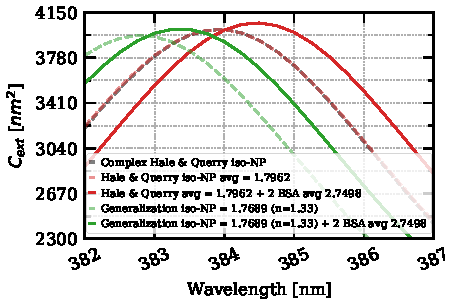
\includegraphics[width=0.85\textwidth]{bsa_phan_avg_real_water_diel.pdf} 
    \caption{Comparison of LSPR response of a silver nanoparticle to two BSA proteins located at $\pm1$ nm on the $z$-direction
    when using a real dielectric model in the protein and the water medium.}
    \label{fig:bsa_w_real}
 \end{figure}

In summary, when studying the LSPR response of a nanoparticle and how it shifts when proteins are in the vicinity, we can use 
real dielectrics for the water medium and the BSA protein, if they come from an average of the real part of the complex dielectric model 
or experimental data (see Hale and Quarry results on Figure \ref{fig:bsa_w_real}). However, when using real-valued dielectrics for the medium 
and the protein, the intensity of the extinction cross section increases, which is a problem if the results are intended to be used for 
sensitivity calculations. 

\section{Reproducibility and data management} \label{sec:repro_ell}
 
All the results of this chapter can be reproduced or replicated. \pygbe is openly developed and 
shared under the BSD3-clause license via its repository at \url{https://github.com/pygbe/pygbe}.

All results of this chapter were obtained on a lab workstation, built from parts. Hardware specifications are as follows:

\begin{itemize}
  \item CPU: Intel Core i7-5930K Haswell-E 6-Core 3.5GHz LGA 2011-v3
  \item RAM: G.SKILL Ripjaws 4 series 32GB (4 x 8GB)
  \item GPU: Nvidia Tesla K40c (with 12 GB memory)
\end{itemize}

Readers can reproduce all the figures in this chapter using the repro-packs shared in Zenodo. They include 
data and scripts needed to run the computations reported in this chapter, as well as Jupyter notebooks with 
all the plotting code:

{\color{red} PENDING}

% Surface Phonon Polaritons resonance: Replication and Validation studies
% !TEX root = ../thesis_main.tex

\chapter{Replication and Validation studies}

HERE WE SHOULD HAVE A PARAGRAPH THAT GOES OVER WHAT WE DID IN THESE 2 CASES
% !TEX root = ../thesis_main.tex

\section{Replicating Rockstuhl et al 2005} \label{chap:rep_rockstuhl}
\graphicspath{{replication_validation/figs/}}

When looking for results to attempt the validation of \pygbe we found the study of Rockstuhl et al. 2005 \cite{rockstuhl2005}. 
Even though their work consist on simulations and therefore does not qualify for a validation study, we decided to 
attempt the replication of one of their results. 

Rockstuhl and coworkers, in their paper "Analysis of the phonon-polariton response of silicon carbide microparticles 
and nanoparticles by use of the boundary element method", study the phonon-polariton response of silicon carbide (SiC)
nanoparticles using boundary element method. They use a two dimensional model developed previously on their group \cite{rockstuhl2003}
to analyze 6H-SiC multiple "cylindrical particles" (third dimension tends to infinity). The results presented on Figure 14 of their paper  
present the scattering cross-section of a SiC rectangular cylinder for different aspect ratios, and the case with $a = 672$ nm and $b = 328$ nm
was a perfect candidate given that these dimensions comply with our quasistatic approach.

In the work of Rockstuhl et al., they compute scattering cross section while with \pygbe we compute the extinction cross-section 
(absorption plus scattering). In the quasistatic regime absorption dominates over scattering, therefore these results are not directly
comparable. However, when having materials which show narrow and sharp peaks on their spectra, the wavelength at which the peaks occur 
in the scattering and extinction spectra, are nearly the same. For example, in the work of Wiley et al. \cite{wiley-etal-2006}
we see that for a silver nanocube, the wavelength at which the main peaks occur for extinction and scattering, are nearly the same. Due to the properties 
of silicon carbide, its spectra presents sharper and narrower peaks than silver, which leads to closely aligned extinction and scattering peaks.


\textbf{Differences in method and input data}

\begin{itemize}

\item {The main difference between the simulations in Rockstuhl and the ones performed with \pygbe is that the original results where obtained 
using a 2D boundary element method that solves full Maxwell equations, while we solve a 3D problem with the quasistatic limit approximation.}

\item{ Rockstuhl et al. work did not have a section with details on their simulations such as discretization of the geometries or parameters 
involved in their simulations. We chose parameters for our solver based on our previous experiences, and for the discretization of our 
geometries we performed a grid-independence study to ensure that we are minimizing discretization errors. It is worth noting that Rockstuhl
et al. geometries consist in two dimensions (infinite third dimension), while we perform the computations using a full 3D representation of the geometry.} 

\item {Regarding the complex dielectric constant, the study we aim to replicate uses 6h-SiC and their data comes from a source that we were not able
to replicate. As a replacement, we are using experimental data of 4H-SiC provided to us by the authors of Ellis et al. \cite{ellis2016} via 
private communications.}

\end{itemize}

\subsection{Grid independence study} \label{ssec:grid_indep_rock}

The equations that we solve in this problem are the same as the ones we solved in chapter \ref{chap:iso_silver_np} where we show grid convergence for the case of 
a silver sphere. In the work of Rockstuhl et al. \cite{rockstuhl2005} the geometries are cubes and prisms, and due to the nature of the geometries 
and their sharp edges, it was hard to find a case where we could see proper convergence using richardson extrapolation. Since we have show convergence for this type of physics
for the case of the sphere and given the difficulty of the sharp edges, we decided to settle with a grid-independence study. We performed the grid-independence study
on a similar setup to the case ib Fig. 18 of Rockstuhl et al. \cite{rockstuhl2005}, a cube of side $L=535$ nm surrounded by air, under a constant electric field aligned with the 
z-axis. Figure \ref{fig:cube535} shows the grid-independence study where we use a mesh with 15,552 triangles and a 19,200 triangles 
(from 9.05 $\times$ 10$^{-5}$ to 1.11 $\times$ 10$^{-4}$ triangles per $\text{\AA}$ squared) and the computed results are indistinguishable from each other.
We want to remark that the spectrum presented in Figure \ref{fig:cube535} has an extra peak compared to the one presented in Fig. 18 of Rockstuhl et al. \cite{rockstuhl2005}. We attribute
this extra peak to the three-dimensional nature of the geometry used in our model and the sharp edges, the latter effect also being mentioned by the Rockstuhl et al.
In the following sections we will present the replication study of one of the results on Figure 14 of Rockstuhl et al. and we will the effects of the 3D model as well as the sharpness of the edges. 

\begin{figure}
    \centering
    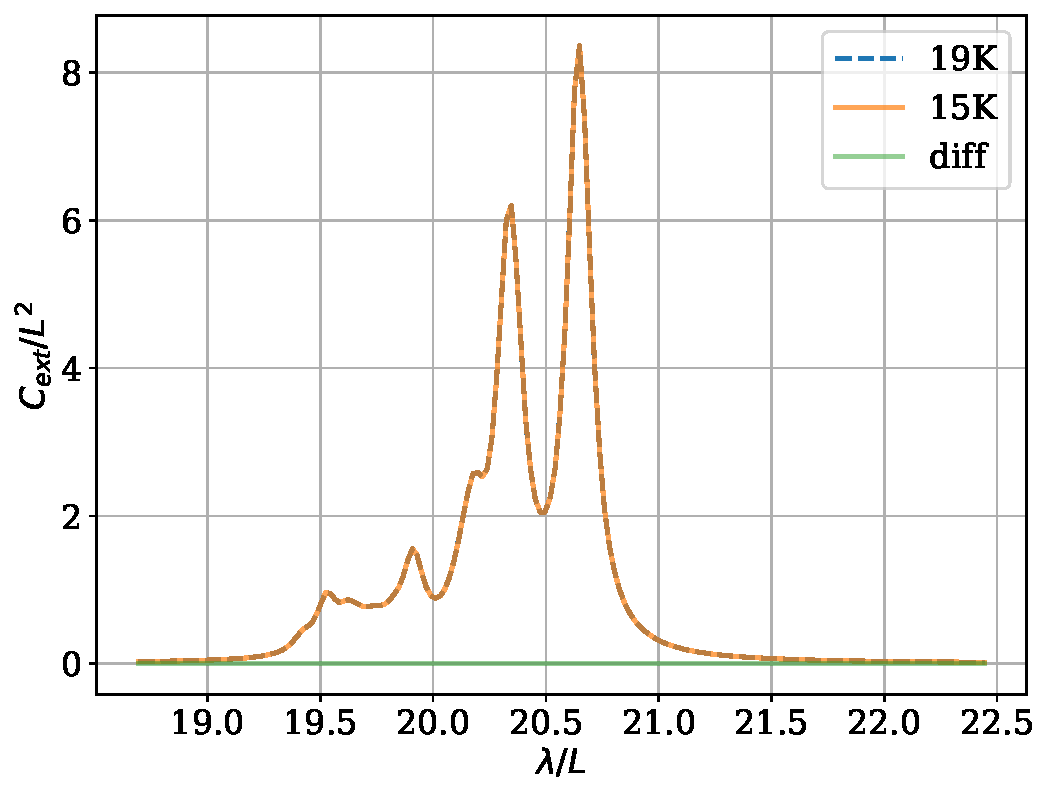
\includegraphics[width=0.75\textwidth]{cubeL535nm_15Kvs19K.pdf} 
    \caption{Grid-independence study for a SiC cube of side $L=535$ nm submerged in air under a constant 
    electric field in the $z$-direction. The curves represent the extinction cross-section divided by $L^2$ 
    as a function of wavelength divided by $L$, for mesh sizes 19K = 19,200 triangles and 15K = 15,552 triangles. 
    The label "diff" refers to the difference between the results of the two meshes.}
    \label{fig:cube535}
 \end{figure}

 \subsection{Replication of Figure 14 (case a1) of Rockstuhl et al., 2005}

 We chose to replicate the case "a1" ($a=672$ nm and $b=328$ nm) from the Figure 14 from Rockstuhl et al., 
 this case has dimensions that are within the quasistatic limit used in \pygbe. Rockstuhl and coworkers show the normalized
 scattering cross-section of a SiC rectangular cylinder, and they perform simulations for the setups showed in the Figure
 \ref{fig:rectangle_sketch}. In Figure \ref{fig:rectangle_sketch} (A) the electric field is parallel to the long side of the geometry, which 
 corresponds to the configuration of Figure 14 (right) of Rockstuhl et al. where the wave vector (illumination) goes along the short side of the geometry. 
Similarly, we see that in Figure \ref{fig:rectangle_sketch} (B) the electric field is parallel to the short side of the geometry, which 
corresponds to the configuration of Figure 14 (left) of Rockstuhl et al. where the wave vector (illumination) goes along the long side of the geometry
For the mesh of the rectangular prisms we used densities like the ones used in the grid-independence study (section \ref{ssec:grid_indep_rock}) or finer. We needed to elongate
the third dimension to the point that it represented "infinity". Figure \ref{fig:ext_y_14} shows the results of extending the third dimension ($y$ axis) to 
$y=1344$ nm ($2\times a$) and $y=2688$ nm ($4\times a$). We can see that when $y$ takes the longer value, the intensity of some peaks decreases, due to their association to 
the y-component. We have not explored larger values of $y$ because are limited by the quasistatic limit.
 \begin{figure}
    \centering
    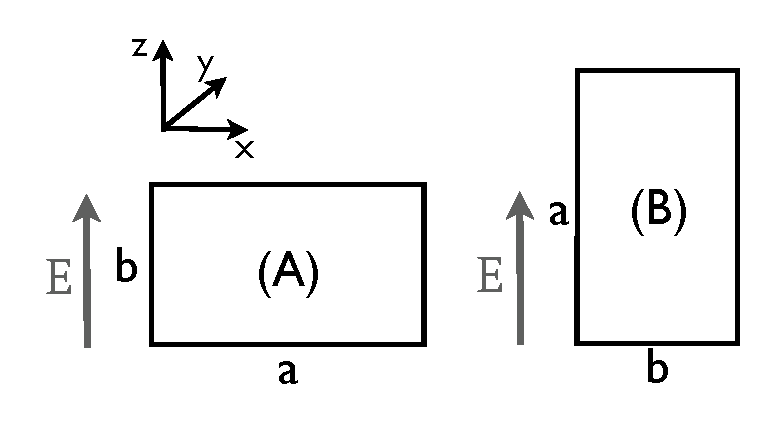
\includegraphics[width=0.45\textwidth]{rockstuhl_rectangles.pdf} 
    \caption{Configurations for the simulations corresponding to Fig. 14 of Rockstuhl et al., 2005.}
    \label{fig:rectangle_sketch}
\end{figure}

\begin{figure}
    \centering
    \subfloat{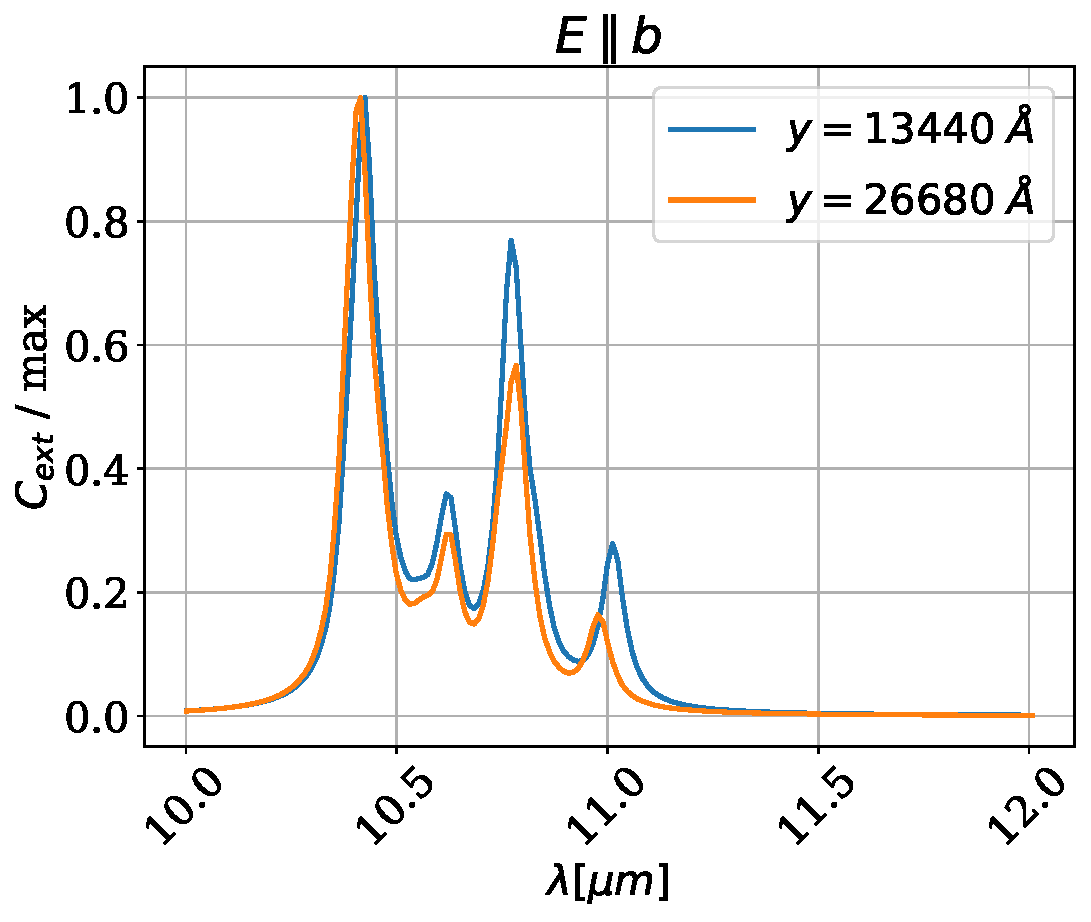
\includegraphics[width=0.48\textwidth]{ext_y_14a.pdf}}
    \subfloat{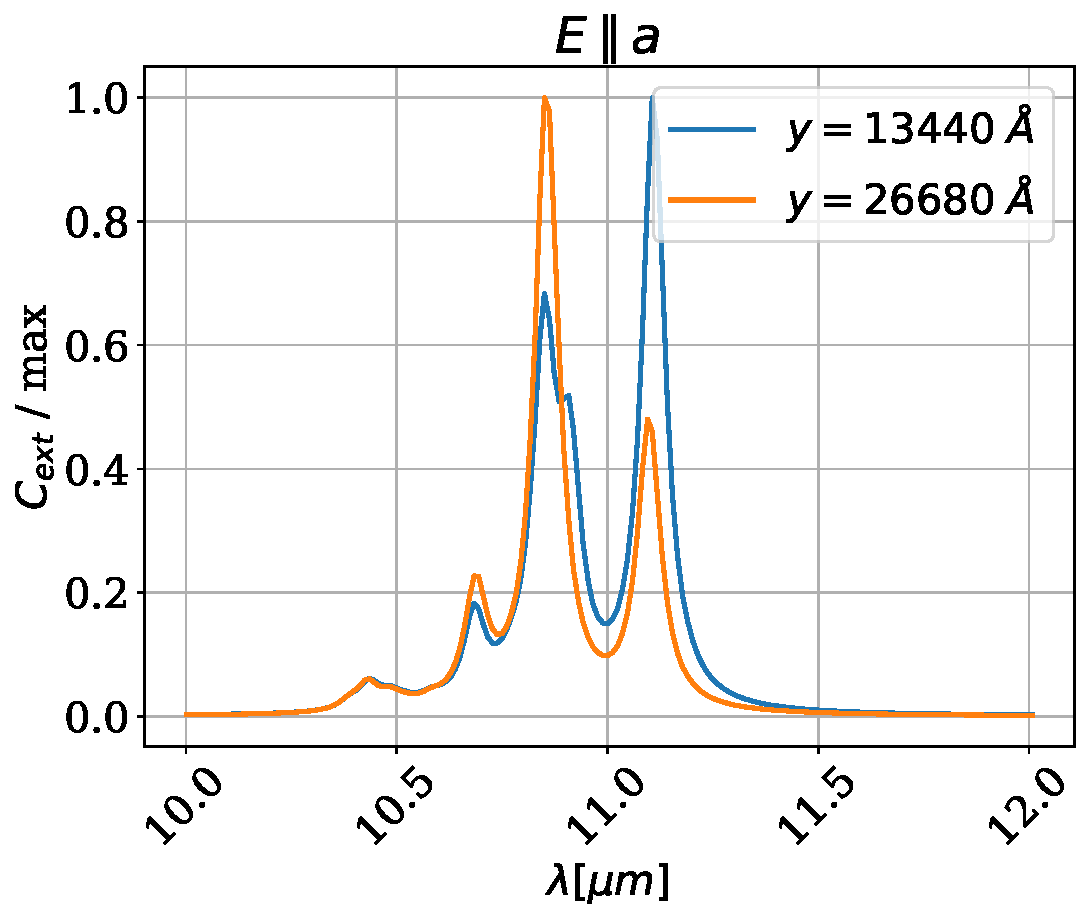
\includegraphics[width=0.48\textwidth]{ext_y_14b.pdf}} 
    \caption{Effect of the elongation of the third dimension ($y$) on the 
        extinction cross-section of a rectangular prism of SiC of dimensions $a=672$ nm 
        and $b=328$ nm, submerged in air and under a constant electric field 
        parallel to the $z$-axis. The left plot corresponds to a configuration such that the electric 
        field is parallel to $b$ (configuration (A) on Figure \ref{fig:rectangle_sketch}), while the 
        right plot corresponds to a configuration such that the electric field is 
        parallel to $a$ (configuration (B) on Figure \ref{fig:rectangle_sketch}.}
    \label{fig:ext_y_14}   
 \end{figure}

For the simulations of Figure \ref{fig:ext_y_14} we generated the meshes using an open source software Trimesh (\url{https://github.com/mikedh/trimesh}), 
but we realized that the mesher did not produce a uniform mesh and that it was not possible to obtained one with the functions available. To solve this problem 
we created a uniform mesh with our own Python script. We wanted to study the effect of using a uniform mesh and the roundness of the edges, the latter being mentioned by 
Rockstuhl et al. as a cause of the appearance of extra peaks. To generate the roundness of the geometries we relied on Trimesh (we give as input the uniform mesh generated 
with our Python script), however, we did not have control of the roundness as a function of the geometry dimensions or arc of curvature, so we used the default settings of
the software. Figure \ref{fig:tri_reg_round_14} shows the results of the effect of mesh uniformity and roundness of the edges of the geometry. We can see that in the for 
both orientation of the geometry ($E\parallel b$ and $E\parallel a$) the second peak located at $\approx$ 10.6 $\mu$m is much diminished in the green curve. These effects 
can be attributed to the roundness of the edges, what is consistent with the results of Rockstuhl et al. Once we have found the "best" meshed geometry (uniform mesh plus 
round edges) that we can construct, we can compare our results (green curve \ref{fig:tri_reg_round_14}) with the ones in Rockstuhl et al. Figure 14. We present the replication 
results in Figure \ref{fig:rep_14}, and we can see that the main resonance peaks in Figure 14 of Rockstuhl et al. are closely matched. We still have a third peak in our 
results, but we attribute this to the effects introduced by using a 3D geometry. We obtained the data from Rockstuhl's curves by using the WebPlotDigitizer
(\url{https://apps.automeris.io/wpd/}).
 

 \begin{figure}
    \centering
    \subfloat{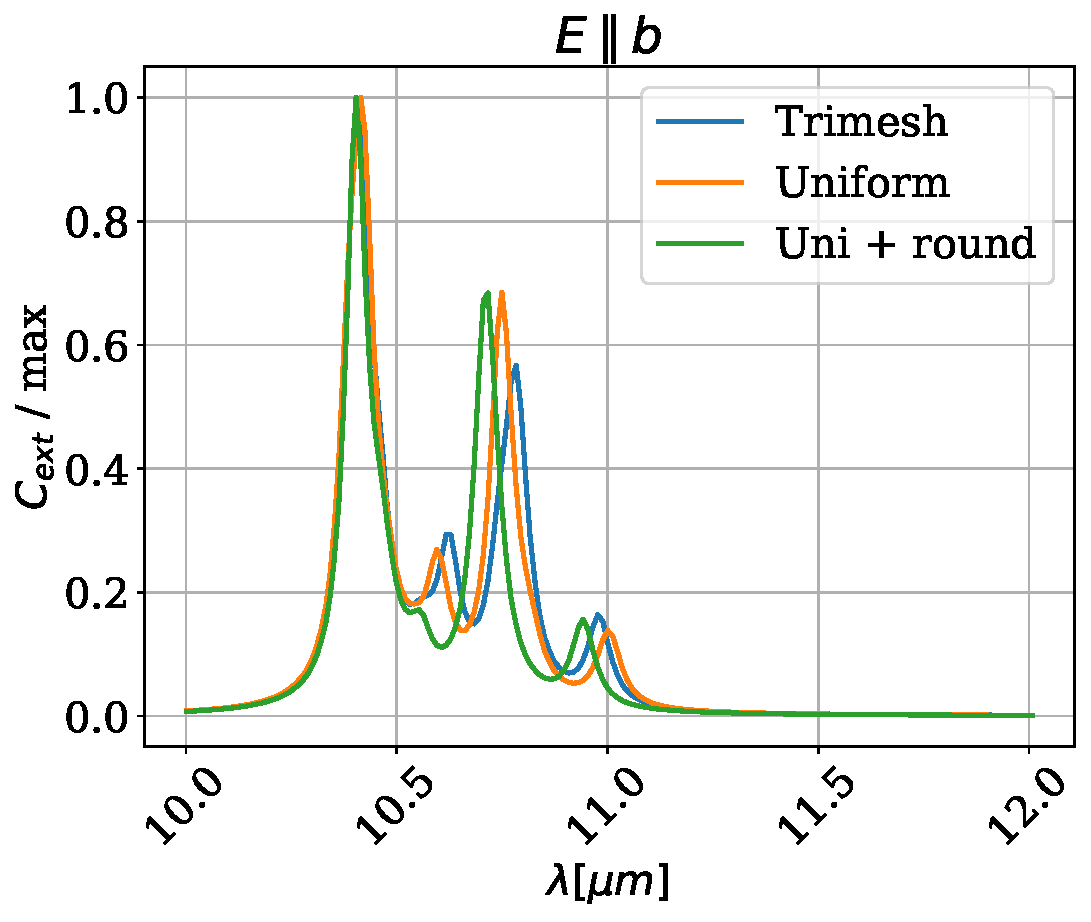
\includegraphics[width=0.48\textwidth]{tri_reg_round_14a.pdf}}
    \subfloat{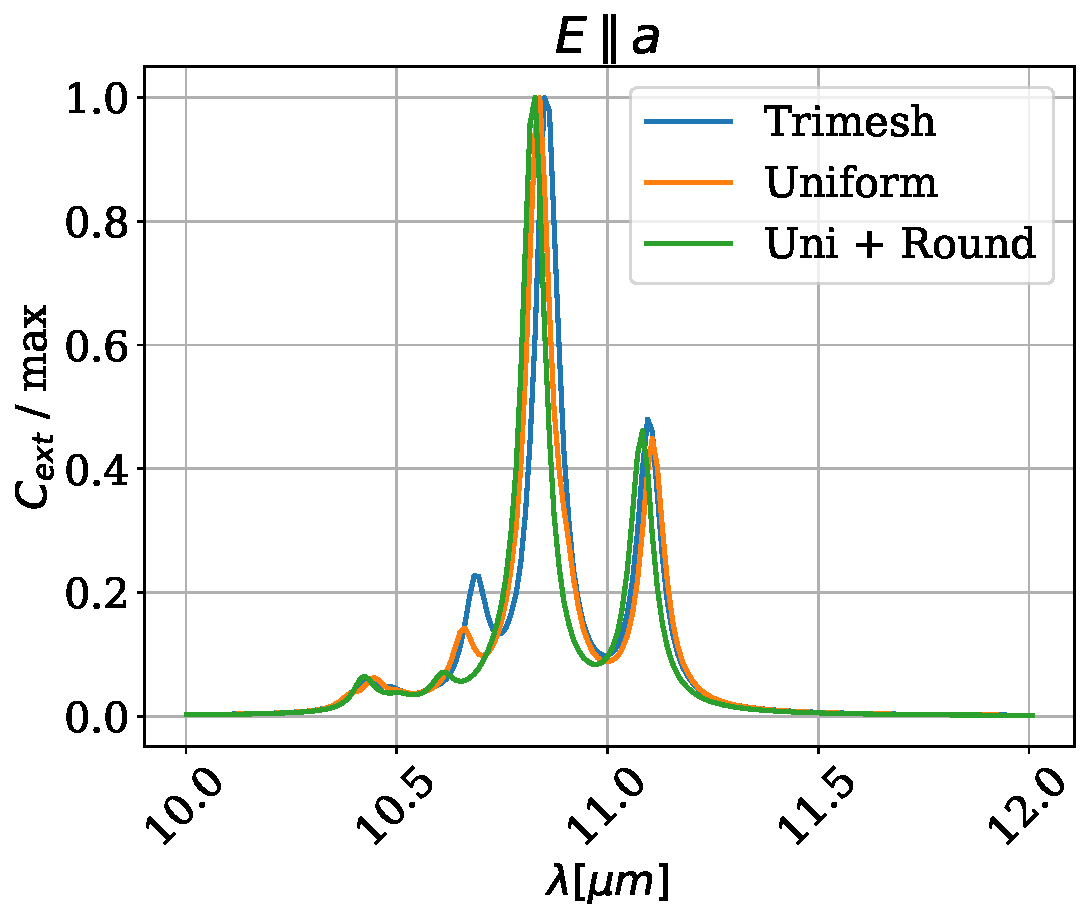
\includegraphics[width=0.48\textwidth]{tri_reg_round_14b.pdf}}
    \caption{Effect of uniformity of the mesh and roundness of the edges on the 
    extinction cross-section of a rectangular prism of SiC of dimensions $a=672$ nm, 
    $b=328$ nm and $y=2688$ nm, submerged in air and under a constant electric field 
    parallel to the $z$-axis. The labels are: \textbf{Trimesh}, for a non-uniform mesh generated using Trimesh; 
    \textbf{Uniform}, for a uniform mesh generated using Python scripts; and 
    \textbf{Uni + round}, for a uniform mesh generated using Python scripts with round 
    edges obtained using Trimesh.}
    \label{fig:tri_reg_round_14}
 \end{figure}

 \begin{figure}
    \centering
    \subfloat{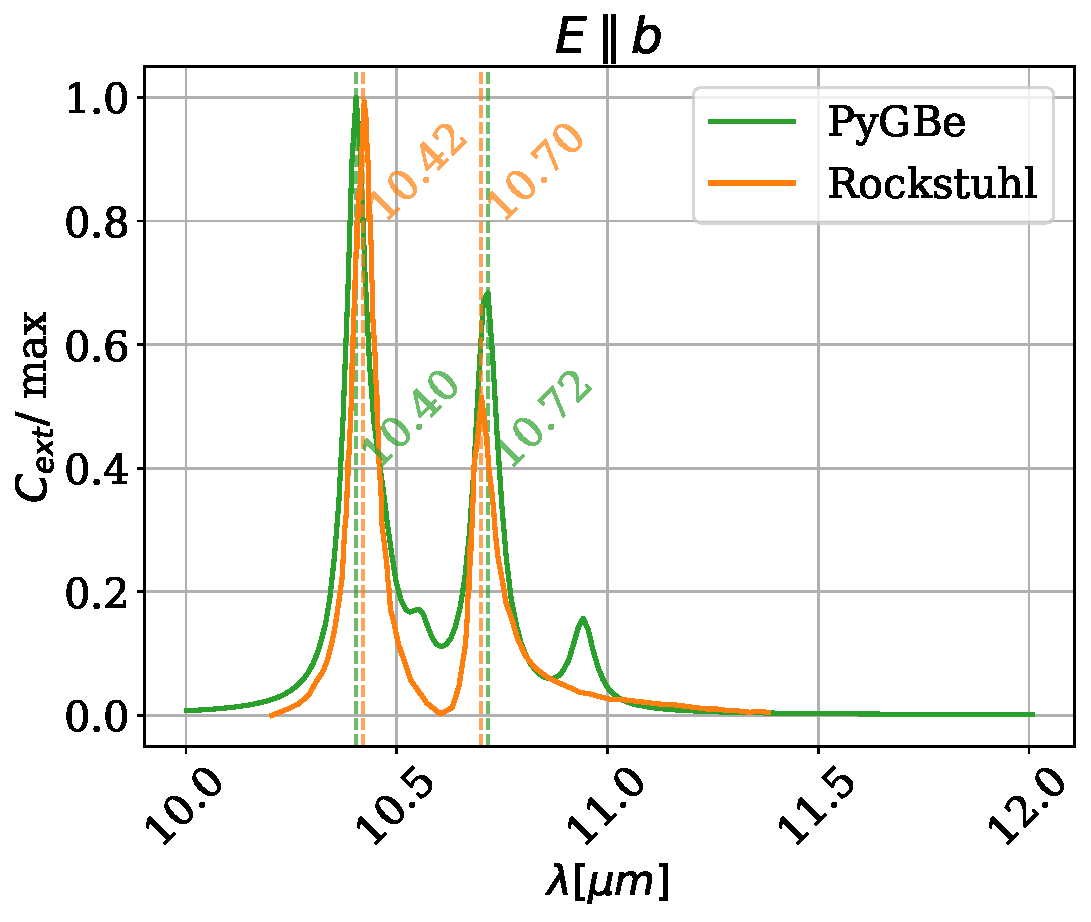
\includegraphics[width=0.48\textwidth]{replication_14a.pdf}}
    \subfloat{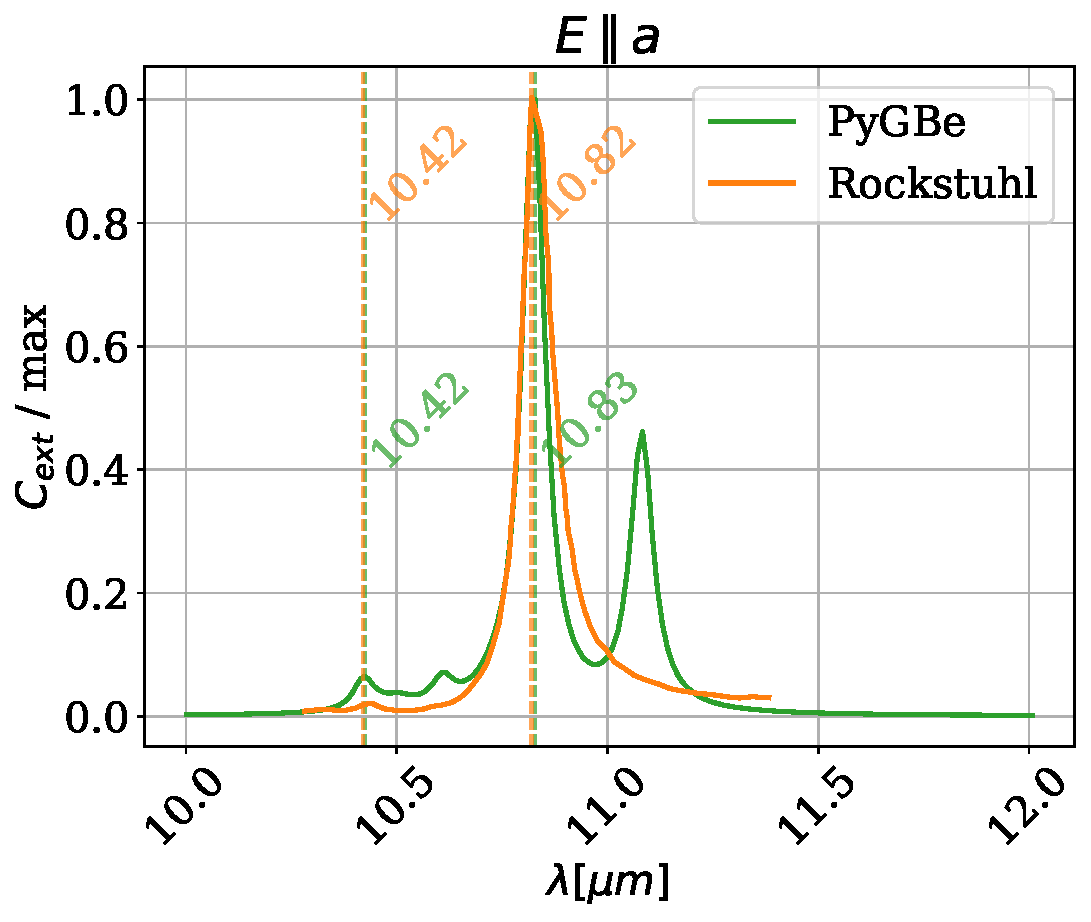
\includegraphics[width=0.48\textwidth]{replication_14b.pdf}} 
    \caption{Replication of the results in Figure 14 of Rockstuhl et al., 2005. Extinction cross-section of a
    rectangular prism of SiC of dimensions $a=672$ nm, $b=328$ nm and $y=2688$ nm, submerged
    in air and under a constant electric field parallel to the $z$-axis (green line). 
    The digitized curve from Rockstuhl et al.\ corresponds to scattering (orange line).}
    \label{fig:rep_14}
 \end{figure}
% !TEX root = ../thesis_main.tex

\section{Validation of \pygbe and Replication of Ellis et al. 2016  et al 2005} \label{sec:rep_val_ellis}
\graphicspath{{replication_validation/figs/}}

The work of Ellis et al. "Aspect-ratio driven evolution of high-order resonant modes and near-field distributions in
localized surface phonon polariton nanostructures." \cite{ellis2016} has both computational and experimental results, that makes 
it a perfect candidate to perform a validation as well as a replication study. Ellis and coworkers study the excitation of 
multipolar localized surface polaritons (SPhP), by computing and measuring the polarized reflectance on 4H-SiC pillars of
fixed width ($W = 400$ nm), fixed height ($H=950$ nm) and varied length ($L=400-4800$ nm). To reduce coupling, these pillars are 
pattern on a square grid with $P = L + 500$ nm. In their experiments (simulations), they measure (compute) the polarized reflectance
where the incident polarization is oriented parallel or perpendicular to the length ($L$) of the pillars. We started by replicating a 
computational result shown in Figure S4 of their supplementary material. Figure S4 of the 
supplementary material shows simulation results for the resonance spectral position of the lower frequency mode when the angle of 
incidence is $22$ degrees and the polarization is parallel to the length of the pillars. They present results for separations of $500$ nm 
(red curve) and $5000$ (black curve), the latter a good candidate for replication with \pygbe because a larger gap diminishes 
the coupling (not included in our model). The setup in our computations consists of a single pillar with no substrate.
Secondly, we aimed to replicate the results of Figure 2a of the main paper, 
corresponding to reflectance measurements across the wave number for pillars of aspect ratio $AR=4$, angle of incidence 22 degrees, 
and incoming parallel polarization. For this case the authors also reported experimental results and we used them for the 
validation of our solver. For all the simulations involved in the replication and validation studies we use experimental values of the 
complex dielectric data for 4H-SIC provided by the authors of Ellis et al. via private communication. 

\textbf{Differences in method and input data}

\begin{itemize}

\item {The simulations of Ellis et al. compute the solution of Maxwell's equations using the RF package
of the finite element solver in the commercial software COMSOL. Their setup consists of one pillar over a 
substrate, with periodic boundary conditions to emulate the array of pillars used in their experiments. In our 
solver we use the boundary element method in the quasistatic approximation, which is suitable since the wavelengths
involved are in the range $10000-12500$ nm, and are considerably larger than the pillar's dimensions. We compute 
the extinction cross section, where the resonance expresses as peaks instead of dips as in the reflection plots of 
Ellis et al. The intensity of the peaks is not comparable, however, we are looking to match the wave number at which
they happen.}

\item {The simulations of Ellis et al. rely on a volumetric model and use a volumetric mesh. In our 
solver, the geometries are represented as a triangular surface meshes. For the validation and replication of Figure 2a of 
their paper, where the pillars have an aspect ratio of $AR=4$, we use a non-uniform triangular mesh ($N=4398$) that 
was provided by the authors of Ellis et al. However, for the replication of the Figure S4 of the supplementary material, 
we were missing the remaining meshes for the other aspect ratios. To overcome this, we generated the meshes with our Python 
script, and we determined the density to be used by comparing simulations for the case of aspect ratio $AR=4$ of our mesh and 
the one provided by Ellis and coworkers. Using approximately double the number of elements ($N=8564$) than the original mesh 
and rounding the edges using Trimesh, the relative errors for the extinction cross-section were, on average, smaller than 
$3\%$, and the variations on the wave number of the peak position was smaller than $1$cm$^-1$. After this analysis we 
concluded in a density of $\approx \; 1.7 \times10^{-5}$ triangles per $\text{\AA}$ squared, which we used to create the meshes
for the remaining aspect ratio geometries.}

\item {In Ellis et al. they perform simulations for different angles of incidence of the illuminating vector. To achieve this 
using \pygbe we rotated the geometry, since the direction of the illuminating vector in our solver is fixed.}
\end{itemize}

\subsection{Replication of Figure S4 of supplementary material of Ellis et al. 2016}

To replicate Figure S4 of the supplementary material we identify the lower-frequency mode for every different 
aspect ratio in our computations. For the values of aspect ratio ($AR$) from 1 to 7, we computed the extinction cross section 
$C_{ext}$ across wave numbers in the range of $800-1000$ cm$^{-1}$, and we identified the lower-frequency mode 
($E^{\parallel}_{100}$ for Ellis et al.) that was not a longitudinal mode. The longitudinal modes are the ones associated with 
the height of the pillar and they appear only when we have an angle of incidence that is off-normal. 
Figure \ref{fig:AR_22_vs_norm} shows the results of the extinction cross-section of a SiC pillar for different values of 
length ($L=400$-$2800$ nm), for normal and 22-degrees angle of incidence (see Figure \ref{fig:ellis_ang_inc}). We performed 
the simulations for the long-edge orientation, meaning that the electric field is aligned with the length of the pillar when having a normal 
incidence. From each result of Figure \ref{fig:AR_22_vs_norm}, we selected the lowest non-longitudinal mode and extracted the corresponding wavelength
(see Table \ref{tab:ar_peaks}) to replicate Figure S4 of the supplementary material of Ellis et al. Figure \ref{fig:rep_FS4_ellis} shows the
results from Ellis et al. (obtained using the WebPlotDigitizer) and the results obtained using \pygbe. Table \ref{tab:err_AR} contains the 
percentage error and we can see that is below 2$\%$ for all the cases.

\begin{figure}
    \centering
    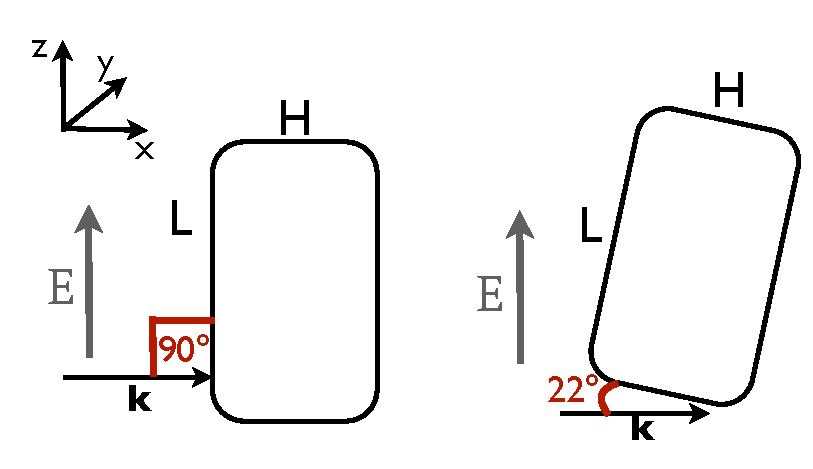
\includegraphics[width=0.45\textwidth]{ellis_ang_inc.pdf} 
    \caption{Diagram showing the angles of incidence in our simulation setups to comply with the configuration in the case from Ellis et al.}
    \label{fig:ellis_ang_inc}
\end{figure}

\begin{figure}
    \centering
    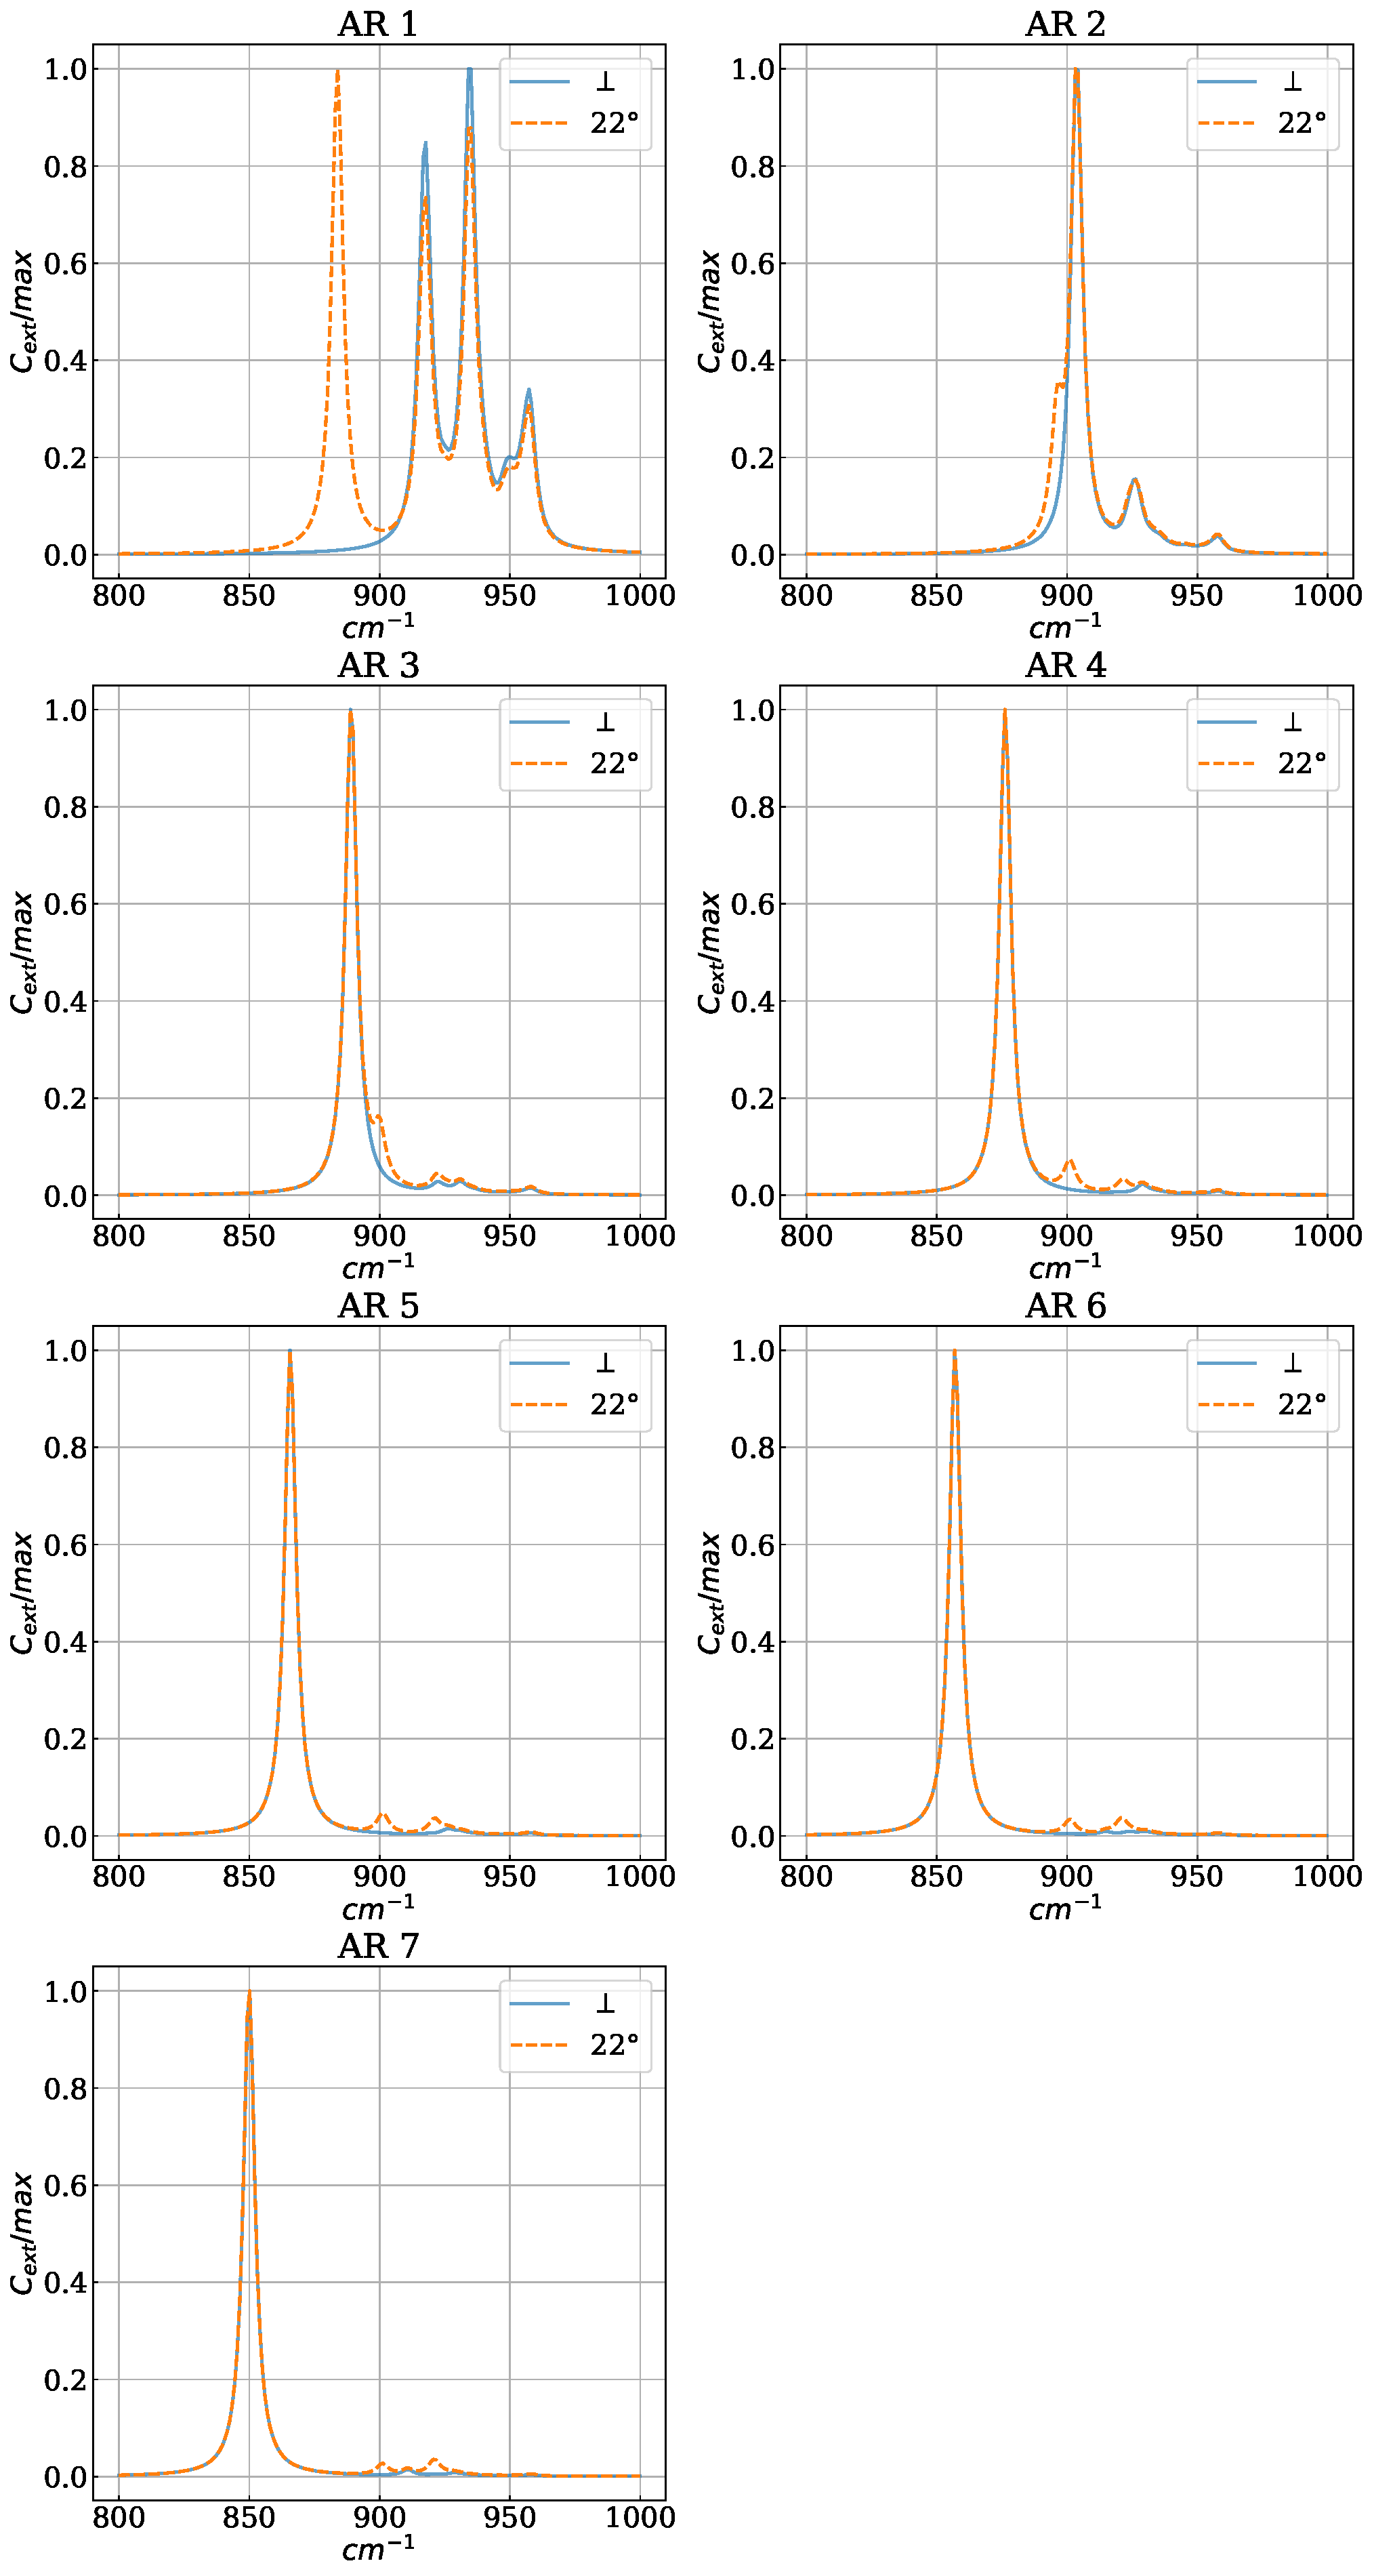
\includegraphics[width=0.72\textwidth]{AR_22_vs_norm.pdf} 
    \caption{Extinction cross-section across wave numbers for SiC pillars of varying aspect ratios,  
             ($H=950$ nm, $W=400$ nm, $L=400$--$2800$ nm, $AR=1$--$7$), with both normal incidence and a 
             22-degree incidence.}
    \label{fig:AR_22_vs_norm}
\end{figure}

\begin{table}
    \centering
      \caption{Wavelength at which peaks happen for different aspect ratios, for runs where the electric
      field is parallel to the length ($L$) of the pillar. We have normal incidence and 22-degree incidence.
      The wavelengths in bold correspond to the lowest mode that is not a longitudinal one.}
      \label{tab:ar_peaks}
      \begin{tabular}{c c c c c c c c}
        \textbf{AR} \\
        \hline
        \multirow{2}{*}{1} & $\perp$ & \textbf{917.73} & 934.092 & 949.604 & 957.325 \\ % <-- Combining 2 rows with arbitrary with (*) and content 12
        & 22$^{\circ}$ & 883.926 & \textbf{917.73} & 935.052 & 949.604 & 957.325 \\ % <-- Content of first column omitted.
        \hline
        \multirow{2}{*}{2} & $\perp$ & \textbf{903.233} & 926.395 & 944.762 & 958.242 \\ % <-- Combining 2 rows with arbitrary with (*) and content 12
        & 22$^{\circ}$ & 896.517 & \textbf{903.233} & 926.395 & 944.762 & 958.242 \\ % <-- Content of first column omitted.
        \hline
        \multirow{2}{*}{3} & $\perp$ & \textbf{888.793} & 922.552 & 931.223 & 948.613 & 958.242 \\ % <-- Combining 2 rows with arbitrary with (*) and content 12
        & 22$^{\circ}$ & \textbf{888.793} & 899.418 & 922.552 & 931.223 & 958.242 \\ % <-- Content of first column omitted.
        \hline
        \multirow{2}{*}{4} & $\perp$ & \textbf{876.186} & 929.32 & 946.639 & 958.242 \\ % <-- Combining 2 rows with arbitrary with (*) and content 12
        & 22$^{\circ}$ & \textbf{876.186} & 901.281 & 921.618 & 929.32 & 945.745 & 958.242 \\ % <-- Content of first column omitted.
        \hline
        \multirow{2}{*}{5} & $\perp$ & \textbf{865.576} & 926.395 & 945.745 & 958.242 \\ % <-- Combining 2 rows with arbitrary with (*) and content 12
        & 22$^{\circ}$ & \textbf{865.576} & 901.281 & 921.618 & 958.242 \\ % <-- Content of first column omitted.
        \hline
        \multirow{2}{*}{6} & $\perp$ &  \textbf{856.904} & 914.793 & 923.489 & 929.32 & 946.639 & 958.242\\ % <-- Combining 2 rows with arbitrary with (*) and content 12
        & 22$^{\circ}$ & \textbf{856.904} & 901.281 & 920.6 & 958.242\\ % <-- Content of first column omitted.
        \hline
        \multirow{2}{*}{7} & $\perp$ &  \textbf{850.134} & 910.963 & 921.618 & 928.372 & 946.639 & 958.242 \\ % <-- Combining 2 rows with arbitrary with (*) and content 12
        & 22$^{\circ}$ & \textbf{850.134} & 901.281 & 910.963 & 920.6 & 958.242\\ % <-- Content of first column omitted.
        \hline
      \end{tabular}
\end{table}

\begin{figure}
    \centering
    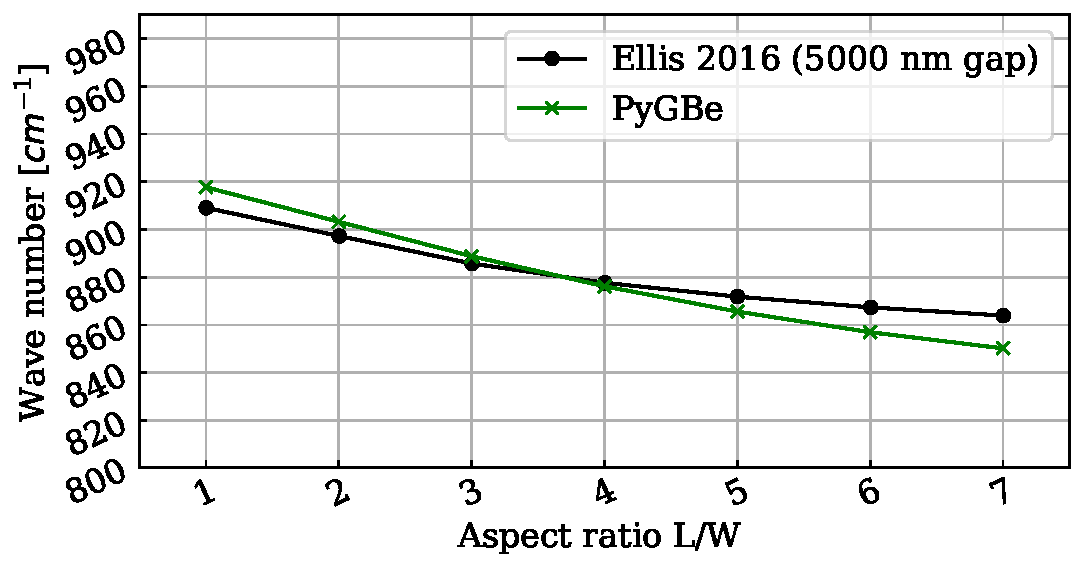
\includegraphics[width=0.85\textwidth]{AR_rep_FS4_Ellis2016.pdf} 
    \caption{Replication of figure S4 in the supplementary materials of Ellis et al., 2016. Wave
    number at which the $E^{\parallel}_{100}$ mode happens for different aspect ratios.}
    \label{fig:rep_FS4_ellis}
 \end{figure}
 
 \begin{table}
    \centering
    \caption{Percentage error for different aspect ratios.} 
    \label{tab:err_AR}
    \begin{tabular}{c c}
    \hline%\toprule
    AR & \% error \\
    \hline%\midrule
     $1$ & $0.95$ \\
     $2$ & $0.67$ \\
     $3$ & $0.35$ \\
     $4$ & $0.16$ \\
     $5$ & $0.72$ \\
     $6$ & $1.20$ \\
     $7$ & $1.59$ \\
    \hline%\bottomrule
    \end{tabular}
\end{table}

\subsection{Validation of \pygbe against experimental results in Fig. 2a of Ellis et al., and replications
of the corresponding computations}\label{ssec:validation}

The geometry used in the results of Figure 2a of Ellis et al. correspond to the case of aspect ratio $AR=4$. For this case,
we have the mesh provided by the authors. Since our computation for the mode $E^{\parallel}_{100}$ compares well with 
their results (percentage error of $0.16\%$), we chose this particular result from Ellis et al. to validate our simulations 
with their experimental results (red curve on their paper), as well as to replicate its corresponding computations (green 
curve on their paper). Figure 2a of Ellis et al. shows experimental and computational results of the reflectance of SiC pillar 
arrays with a gap of 500 nm, where the angle of incidence is 22$^\circ$ off-normal and the incoming polarization is parallel 
to the length of the pillar. Using \pygbe, we computed the extinction cross section of an isolated SiC pillar of aspect ratio
$AR=4$ with no substrate, submerged in air and under a constant electric field in the $z$-direction. The geometry was rotated to match
the angle of incidence of 22$^\circ$ used by Ellis et al. (see Figure \ref{fig:ellis_ang_inc}). Figure \ref{fig:pygbe_vs_exp_2a} 
shows the comparison of our simulations and the experimental results of Ellis et al. We can observe a noticeable difference in between 
the wave numbers at which the peaks occur. This difference may be attributed to the fact that in their experimental setup the 
separation between the pillars is $500$ nm, which implies there are coupling effects that are not considered in our simulations.

\begin{figure}
    \centering
    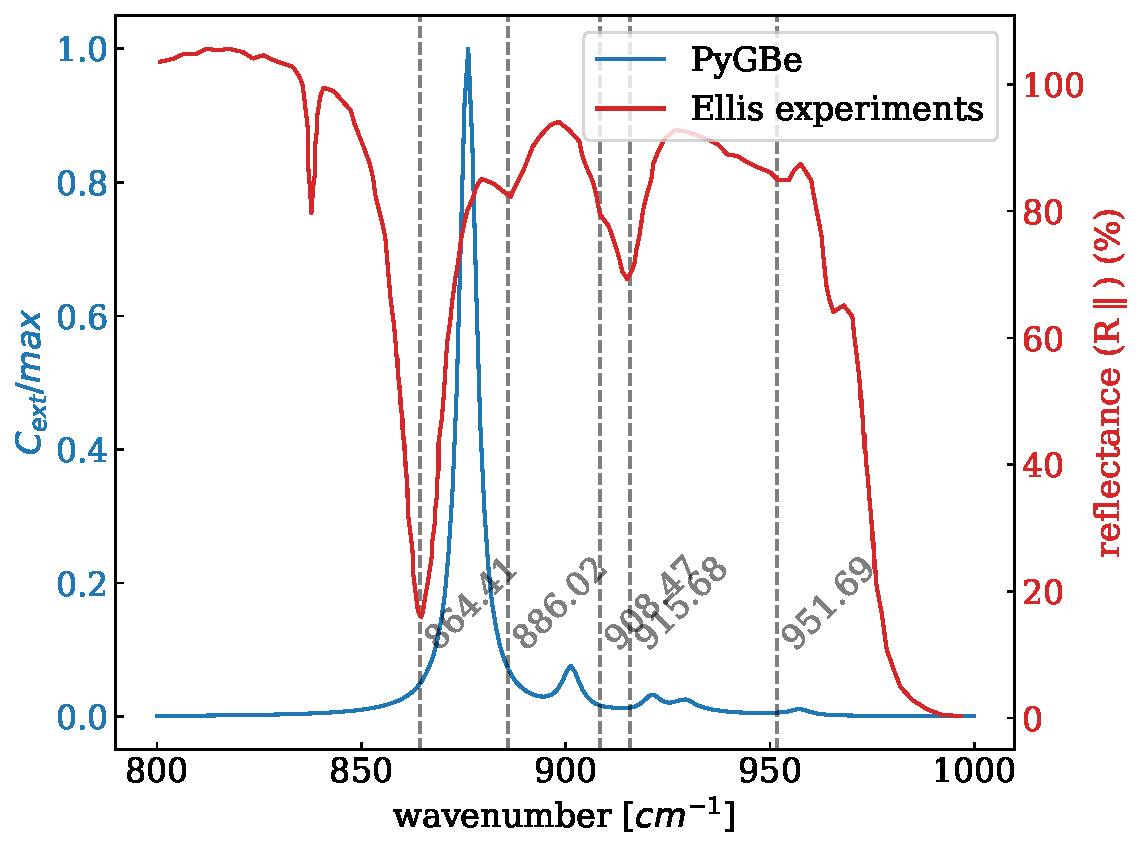
\includegraphics[width=0.85\textwidth]{pygbe_vs_exp_fig2a_Ellis.pdf} 
    \caption{\pygbe vs.\ the experiments presented in Figure 2a of Ellis et al., 2016 (we obtained the data 
    digitizing by hand from their figure using WebPlotDigitizer).}
    \label{fig:pygbe_vs_exp_2a}
 \end{figure}

\textbf{First-order correction.} 

Since our simulations are performed on an isolated prism and do not take into account the coupling effects 
in an array of prisms, we cannot strictly match the conditions to validate our solver. However, from Figure S4 in the supplementary material of 
Ellis et al., we know that this coupling effects affect the $E^{\parallel}_{100}$ mode by a shift of 12.17 cm$^{-1}$. Then, as a 
\textbf{first-order correction}, we can subtract this amount from our computations to account for the coupling effects. Figure \ref{fig:val_2a}, 
shows the results after applying the correction. It is worth mentioning that the peaks at 837 cm$^{-1}$) and (964 cm$^{-1}$) on the results of Ellis et al., 
are associated with the zone-folded LO (longitudinal) phonons of 4H-SiC, an effect they say to be beyond the scope of their analysis \cite{ellis2016}. Their 
analysis concentrates on the peaks that occur between 864 cm$^{-1}$ and 961 cm$^{-1}$. 
Figure \ref{fig:rep_2a} shows the comparison between Ellis et al. simulation's results on Figure 2a of their paper (green curve), and our computations
after applying the first-order correction.

\begin{figure}
    \centering
    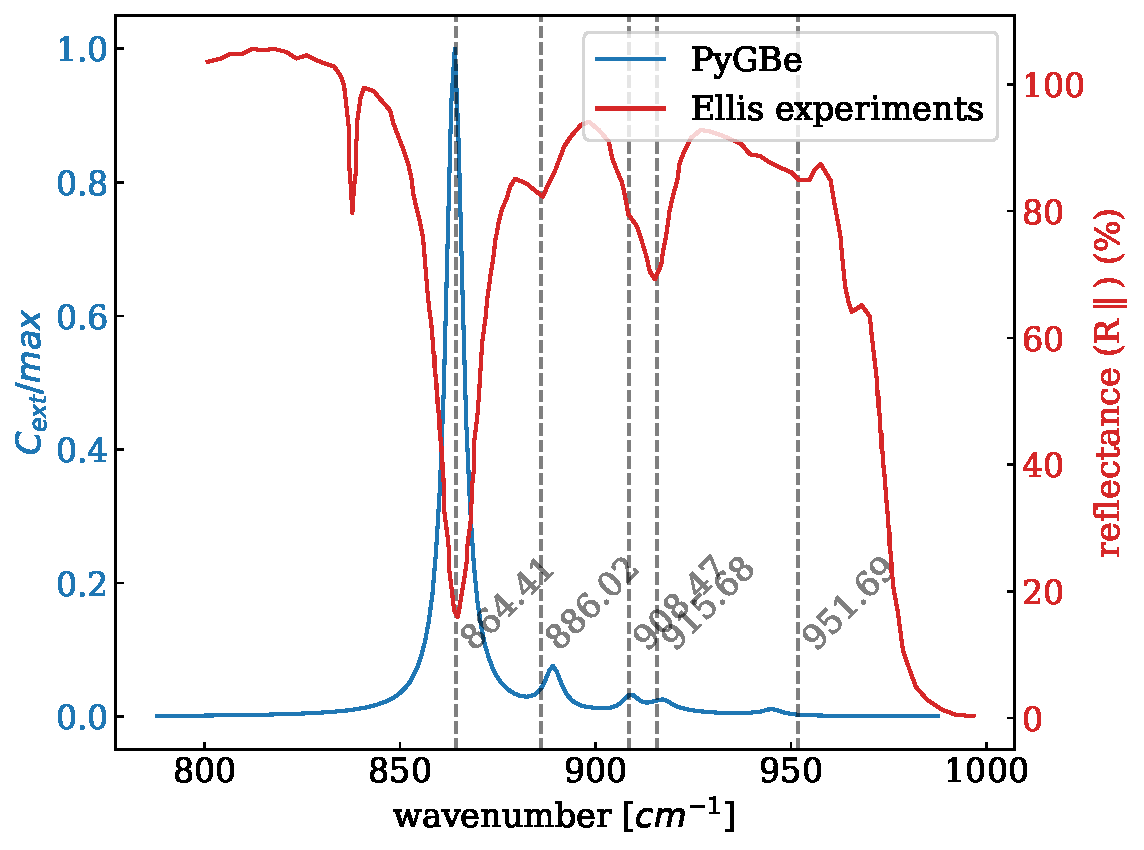
\includegraphics[width=0.85\textwidth]{validation_FOA_fig2a_Ellis.pdf} 
    \caption{Validation against experiments in Figure 2a of Ellis, et al., 2016, using the first-order correction, as explained in the text.}
    \label{fig:val_2a}
 \end{figure}

\begin{figure}
    \centering
    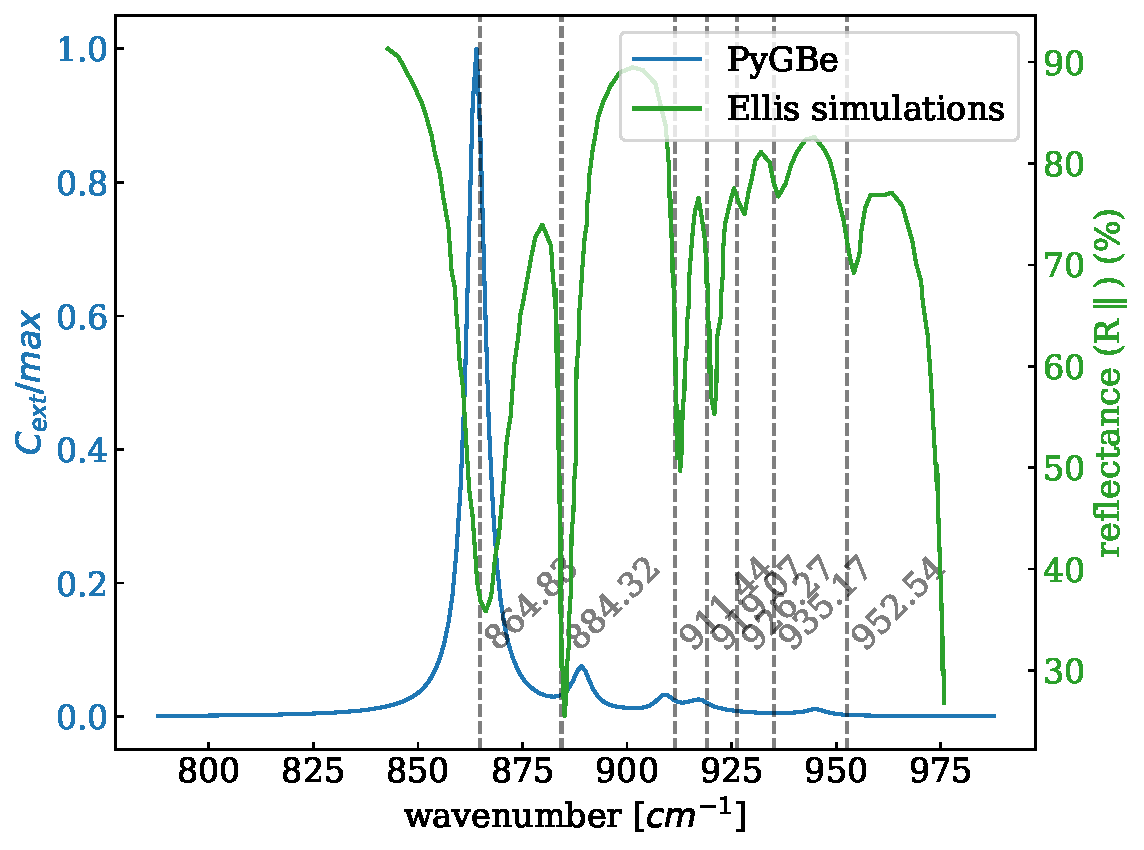
\includegraphics[width=0.85\textwidth]{replication_FOA_fig2a_Ellis.pdf} 
    \caption{Replication of the simulations in Figure 2a of Ellis et al., 2016, using the first-order correction, as explained in the text.}
    \label{fig:rep_2a}
 \end{figure}


In this section, we attempted to replicate two results from Ellis et al. \cite{ellis2016} where they study the effect of aspect ratio on the 
excitation of high-order modes in localized surface phonon-polariton nanostructures. Figure \ref{fig:rep_FS4_ellis} shows the results for
the replication of the black curve of Figure S4 of their supplementary material, where the relative errors between our computations and 
theirs is always smaller than 2$\%$. This replication study gave us the confidence to approach the replication of Figure 2a of Ellis et al., 
given that in that case they use a geometry with aspect ratio $AR=4$ presented the smallest error (see Table \ref{tab:err_AR}). Since 
Figure 2a of Ellis et al. shows results of experiments and simulations with the commercial software COMSOL, we not only pursued replication 
but we also sought the validation of \pygbe using these experimental results. The quantity plotted in the original figures is reflectance as a 
function of wavenumber, while we compute the extinction cross section. Since the quantity of interest is the wavenumber at which the resonance 
peaks/dips happen, the results are comparable. 

Figure \ref{fig:pygbe_vs_exp_2a} shows the results of our simulations using \pygbe on an isolated pillar, compared with the experimental results
of Ellis et al.\ on an array of pillars. The results with \pygbe do not account for the effect of coupling among the pillars, which explains the  
discrepancy on the wavenumbers at which the peaks occur. It is worth mentioning that we did not count with the original data behind the plots of 
Ellis et al. therefore, we digitize the curves using the WebPlotDigitizer(\url{https://apps.automeris.io/wpd/}). Based on the results reported 
on Figure S4 of Ellis et al.\ for the $AR=4$ case, we proposed a first order correction that subtract the shift on the wave number due to
coupling is 12.17 cm$^{-1}$ (difference between black and red curves for $AR=4$ on figure S4 of the supplementary materials). Figure \ref{fig:val_2a}
and Figure \ref{fig:rep_2a} show the comparison of our corrected results with their experiments and simulations, respectively. We observe a good match 
of the wavenumber for the lower (and stronger) mode, as well as a good match for the third and fourth peaks. The wave number of the second peak, related 
to a longitudinal excitation (mode $L_{000}$ in Ellis et al.), presents a discrepancy that we believe is related to the fact that our 
pillar does not have a substrate underneath. The remaining (fifth) peak, also presents a discrepancy, but in this case we could not identify the reason.
We did not analyze the peaks out of the range 864--961 cm$^{-1}$, since Ellis et al.\ describe these peaks to be associated with 
zone-folded LO (longitudinal) phonons of 4H-SiC, and outside the scope of their study.
After considering all these details, we can say that we have validated our solver \pygbe against the experimental results of 
Figure 2a, as well as replicated their computational results.

\section{Reproducibility and data management} \label{sec:repro_val}
 
All the results of this chapter have been accepted for publication in the journal 
Philosophical Transactions A \cite{ClementiBarba2020} and can be reproduced or replicated. \pygbe is openly developed and 
shared under the BSD3-clause license via its repository at \url{https://github.com/pygbe/pygbe}.

All results of this chapter were obtained on a lab workstation, built from parts. Hardware specifications are as follows:

\begin{itemize}
  \item CPU: Intel Core i7-5930K Haswell-E 6-Core 3.5GHz LGA 2011-v3
  \item RAM: G.SKILL Ripjaws 4 series 32GB (4 x 8GB)
  \item GPU: Nvidia Tesla K40c (with 12 GB memory)
\end{itemize}

Readers can reproduce all the figures in this chapter using the repro-packs shared in Zenodo. They include 
data and scripts needed to run the calculations reported in this chapter, the manually digitized data from the figures
in the source articles for our replication cases, as well as Jupyter notebooks with all the plotting code:

\begin{itemize}

\item[$\triangleright$] The problem datasets for replication of Rockstuhl et al., 2005, are in the manuscript repository, but also archived in Zenodo  at \href{https://doi.org/10.5281/zenodo.3962534}{10.5281/zenodo.3962534}  \cite{ClementiBarba2020-Zen_a}.

\item[$\triangleright$] Execution files for all runs are archived in Zenodo at \href{https://doi.org/10.5281/zenodo.3962576}{10.5281/zenodo.3962576} \cite{ClementiBarba2020-Zen_b}.

\item[$\triangleright$] The problem datasets for validation and replication of results from Ellis et al., 2016 are archived in Zenodo at \href{https://doi.org/10.5281/zenodo.3962584}{10.5281/zenodo.3962584}\cite{ClementiBarba2020-Zen_c}.

\item[$\triangleright$] The file sets for reproducing the figures for the replication of results from Rockstuhl et al., 2005 are archived in Zenodo at \href{https://doi.org/10.5281/zenodo.3962791}{10.5281/zenodo.3962791} \cite{ClementiBarba2020-Zen_d}.

\item[$\triangleright$] The file sets for reproducing the figures for the validation and replication of results from Ellis et al., 2017 are archived in Zenodo at \href{https://doi.org/3962797/zenodo.3962797}{10.5281/zenodo.3962797} \cite{ClementiBarba2020-Zen_e}.

\end{itemize}


%conclusions
% !TEX root = ../thesis_main.tex
\chapter{Conclusions}

In this work, we extended the implicit-solvent model of electrostatics implemented in \pygbe \cite{CooperClementiBarba2015}
to study nanoplasmonics in the quasistatic limit for applications in biosensing \cite{ClementiETal2017, ClementiETal2019}.
We applied this model to simulations of localized surface plasmon resonance, where we computed the extinction cross section of 
conductive nanoparticles and computed the shift in the resonance frequency when having biomolecules in the vicinity of the 
nanoparticle.

\textbf{Contributions of this work}

We developed an open source boundary integral solver for computational nanoplasmonics in the quasistatic limit. We extended \pygbe to work 
with complex values, and added the functionality needed to solve localized surface plasmon resonance problems. \pygbe 
counts with an algorithmic acceleration with a treecode, and hardware acceleration with GPUs, making this solver 
suitable to compute problems of at least a half million boundary elements, which is required to represent the solvent excluded 
surface of the biomolecule accurately.

We verified our solver against an analytical solution based on the Mie theory for silver nanospheres (section \ref{sec:verification}), and 
presented convergence studies for our results, building confidence on the suitability of our boundary integral model and the  
correctness of our solver. We performed a sensitivity study of an LSPR biosensor model by computing the resonance-frequency shift
while varying the distance between the nanoparticle and the biomolecules. We showed that our boundary element methods approach in
the quasistatic limit can capture the characteristic behavior of LSPR biosensors (section \ref{sec:lspr_response_bsa}).

We explored different reduced-order models for the protein, and showed that geometries like ellipsoids and spheres
are not accurate models for the protein representation compared to using a meshed constructed from its crystal structure. Even though
none of these models were accurate, the volume equivalent ellipsoidal model performed better compared to the surface based ellipsoidal 
model and the volume equivalent spherical model. Using volume equivalent ellipsoids for the protein representation 
translated to fast computations, that even if they were not accurate compared to the full model, they served as great candidates to
explore the different components of the computational model of the biosensor. We used this model to shine light on the effects of multiple factors such as 
the orientation of the protein, the presence of charges in the protein, the number of proteins, and the effect of the incoming electric field \ref{sec:ell_study}.
We found that using real dielectrics for the protein and the embedding medium does not affect the shift in the resonance frequency, 
as long as they are averaged values from the real part of the original complex data. However, using real dielectrics does affect the 
intensity of the extinction cross section, which is a problem if the results are intended to be used for sensitivity calculations \ref{sec:diel_study}. 
These reduced-order models, despite not being accurate compared to the full protein model, provide fast computed insights that can be used 
in the exploratory stage on the design or study of biosensors.

We matched and replicated the findings of computational results in the general area of nanostructure responses to electromagnetic waves 
from Rockstuhl et al. \cite{rockstuhl2005} and Ellis et al.\cite{ellis2016} (section \ref{sec:rep_rockstuhl} and \ref{sec:rep_val_ellis}). We validated
\pygbe against experimental results of reflectance of localized surface phonon polariton (SPhP) nanostructures from Ellis et 
al. (section \ref{sec:rep_val_ellis}). Both replication and validation studies were difficult to achieve due to insufficient data and experiments 
and/or simulation details, and we stated that the lack of reproducible open practices is the primary cause. We concluded that open reproducible 
practices are needed not only to guarantee the work published is possible to reproduce, but also for future replicability and validation studies. 

All of the results of this work, along with the materials needed to reproduce or replicate them, are publicly available in the form of 
reproducibility packages (sections \ref{sec:repro_lspr}, \ref{sec:repro_ell}, and \ref{sec:repro_val}). The nanoplasmonics extension of \pygbe, and 
the results of this work, can offer a valuable computational approach for the future studies on the field, and aid in the design of LSPR biosensors 
as well as SPhP based sensors. 





\bibliographystyle{unsrt}
\bibliography{thesis_ncc_bib}

% appendices must appear after
%\include{tex/appendix}
\end{document}
